\documentclass[11pt]{article}
\usepackage[a4paper,left=22mm,right=22mm,top=23mm,bottom=25mm]{geometry}
\usepackage{graphicx}
\usepackage{url}
\usepackage{hyperref}
\usepackage{amsmath}
\usepackage{fancyhdr}
\usepackage[czech]{babel}
\usepackage[utf8]{inputenc}
\hypersetup{colorlinks=true,linkcolor=blue,urlcolor=blue}

\begin{document}
\clubpenalty 10000
\widowpenalty 10000

\title{5. Řešení problému vážené splnitelnosti booleovské formule pokročilou iterativní metodou}
\author{Ladislav Martínek}
\date{}
\maketitle
 
\section{Problém} \label{kap:problem}
 Je dána booleovská formule $F$ proměnnných $X=(x_1, x_2, \dots, x_n)$ v konjunktivní normální formě (tj. součin součtů). Dále jsou dány celočíselné kladné váhy $W=(w_1, w_2, \dots, w_n).$ Najděte ohodnocení $Y=(y_1, y_2, \dots, y_n)$ proměnných $x_1, x_2, \dots, x_n$ tak, aby $F(Y)=1$ a součet vah proměnných, které jsou ohodnoceny jedničkou, byl maximální.

Je přípustné se omezit na formule, v nichž má každá klauzule právě 3 literály (problém 3 SAT). Takto omezený problém je stejně těžký, ale možná se lépe programuje a lépe se posuzuje obtížnost instance (viz Selmanova prezentace v odkazech).
 
 
\section{Zadání úlohy} \label{kap:zadani}

Problém řešte některou z pokročilých lokálních heuristik (simulované ochlazování, genetické algoritmy, tabu prohledávání). Řešení jinými metodami prosím zkonzultovat se cvičícím nebo předná\-šejícím. Volby konkrétních parametrů heuristiky a jejích detailů (operace nad stavovým prostorem, kritérium ukončení, atd. atd.) proveďte sami, tyto volby pokud možno zdůvodněte a ověřte experimentálním vyhodnocením. Hodnocení Řešení této úlohy je podstatnou součástí hodnocení zkoušky (28 bodů ze 100). Hodnotí se především postup při aplikaci heuristiky, tj. postup a experimenty, jakým jste dospěli k výsledné podobě (parametry, konkrétní operátory apod.). Například, pokud máte v řešení nějaké hodně neortodoxní prvky a pokud máte jejich výhodnost experimentálně doloženou, těžko mohou vzniknout námitky. Méně významné jsou konkrétní dosažené výsledky. Nežádáme rozhodně, aby semestrální práce měla úroveň světové výzvy Centra diskrétní matematiky Rutgersovy univerzity.

Tato práce by měla sloužit jako ověření Vašich schopností používat zvolenou pokročilou iterativní metodu. Ideálním výstupem by měl být algoritmus schopný řešit co nejširší spektrum instancí s~rozumnou chybou. To neznamená, že pokud se Vám některé instance "nepovedou", je vše špatně. Důležité je, abychom viděli, že jste se aspoň snažili. Někdy to prostě nejde...

\section{Rozbor zadaného problému}\label{kap:rozbor}

\section{Popis implementovaného genetického algoritmu}\label{kap:popisALG}

\section{Implementace}\label{kap:implementace}

\section{Testovací data}\label{kap:data}

\section{Testovací platforma}\label{kap:platform}

\subsection{Cíle}\label{kap:cil}

Vlastnosti algoritmu lze měnit pomocí parametrů, jako je počáteční teplota, ochlazování a~počet iterací na jedné teplotě. Při řešení tohoto problému, jsem neuvažoval neplatná řešení, jelikož začínám s~prázdným batohem. Cílem je otestovat chování algoritmu v závislosti na těchto parametrech a~vyvodit závěry. Tedy se naučit iterativní heuristiku nastavit na tento problém a~řešit ho pomocí ní. 


\section{Experimenty}\label{kap:experiments}


Experimenty jsem prováděl v režimu jednoho vlákna na starším datovém serveru v podobě starého notebooku, který v době výpočtu nebyl používán. Výsledky tedy nejsou ovlivněny jinými běžícími programy. Procesor na testovacím stroji: \textit{Intel Pentium T3400 (2 cores). Taktován na 2.16~GHz s~1~MB cache}.
Měření času CPU probíhalo v~knihovně $timeit$. Algoritmus jsem napsal v~Cythonu a~časy tedy nemohou být případně srovnávány s~řešením v~předchozích úlohách.

 


\begin{figure}
	\centering
    \begin{minipage}[c]{0.42\textwidth}
        \centering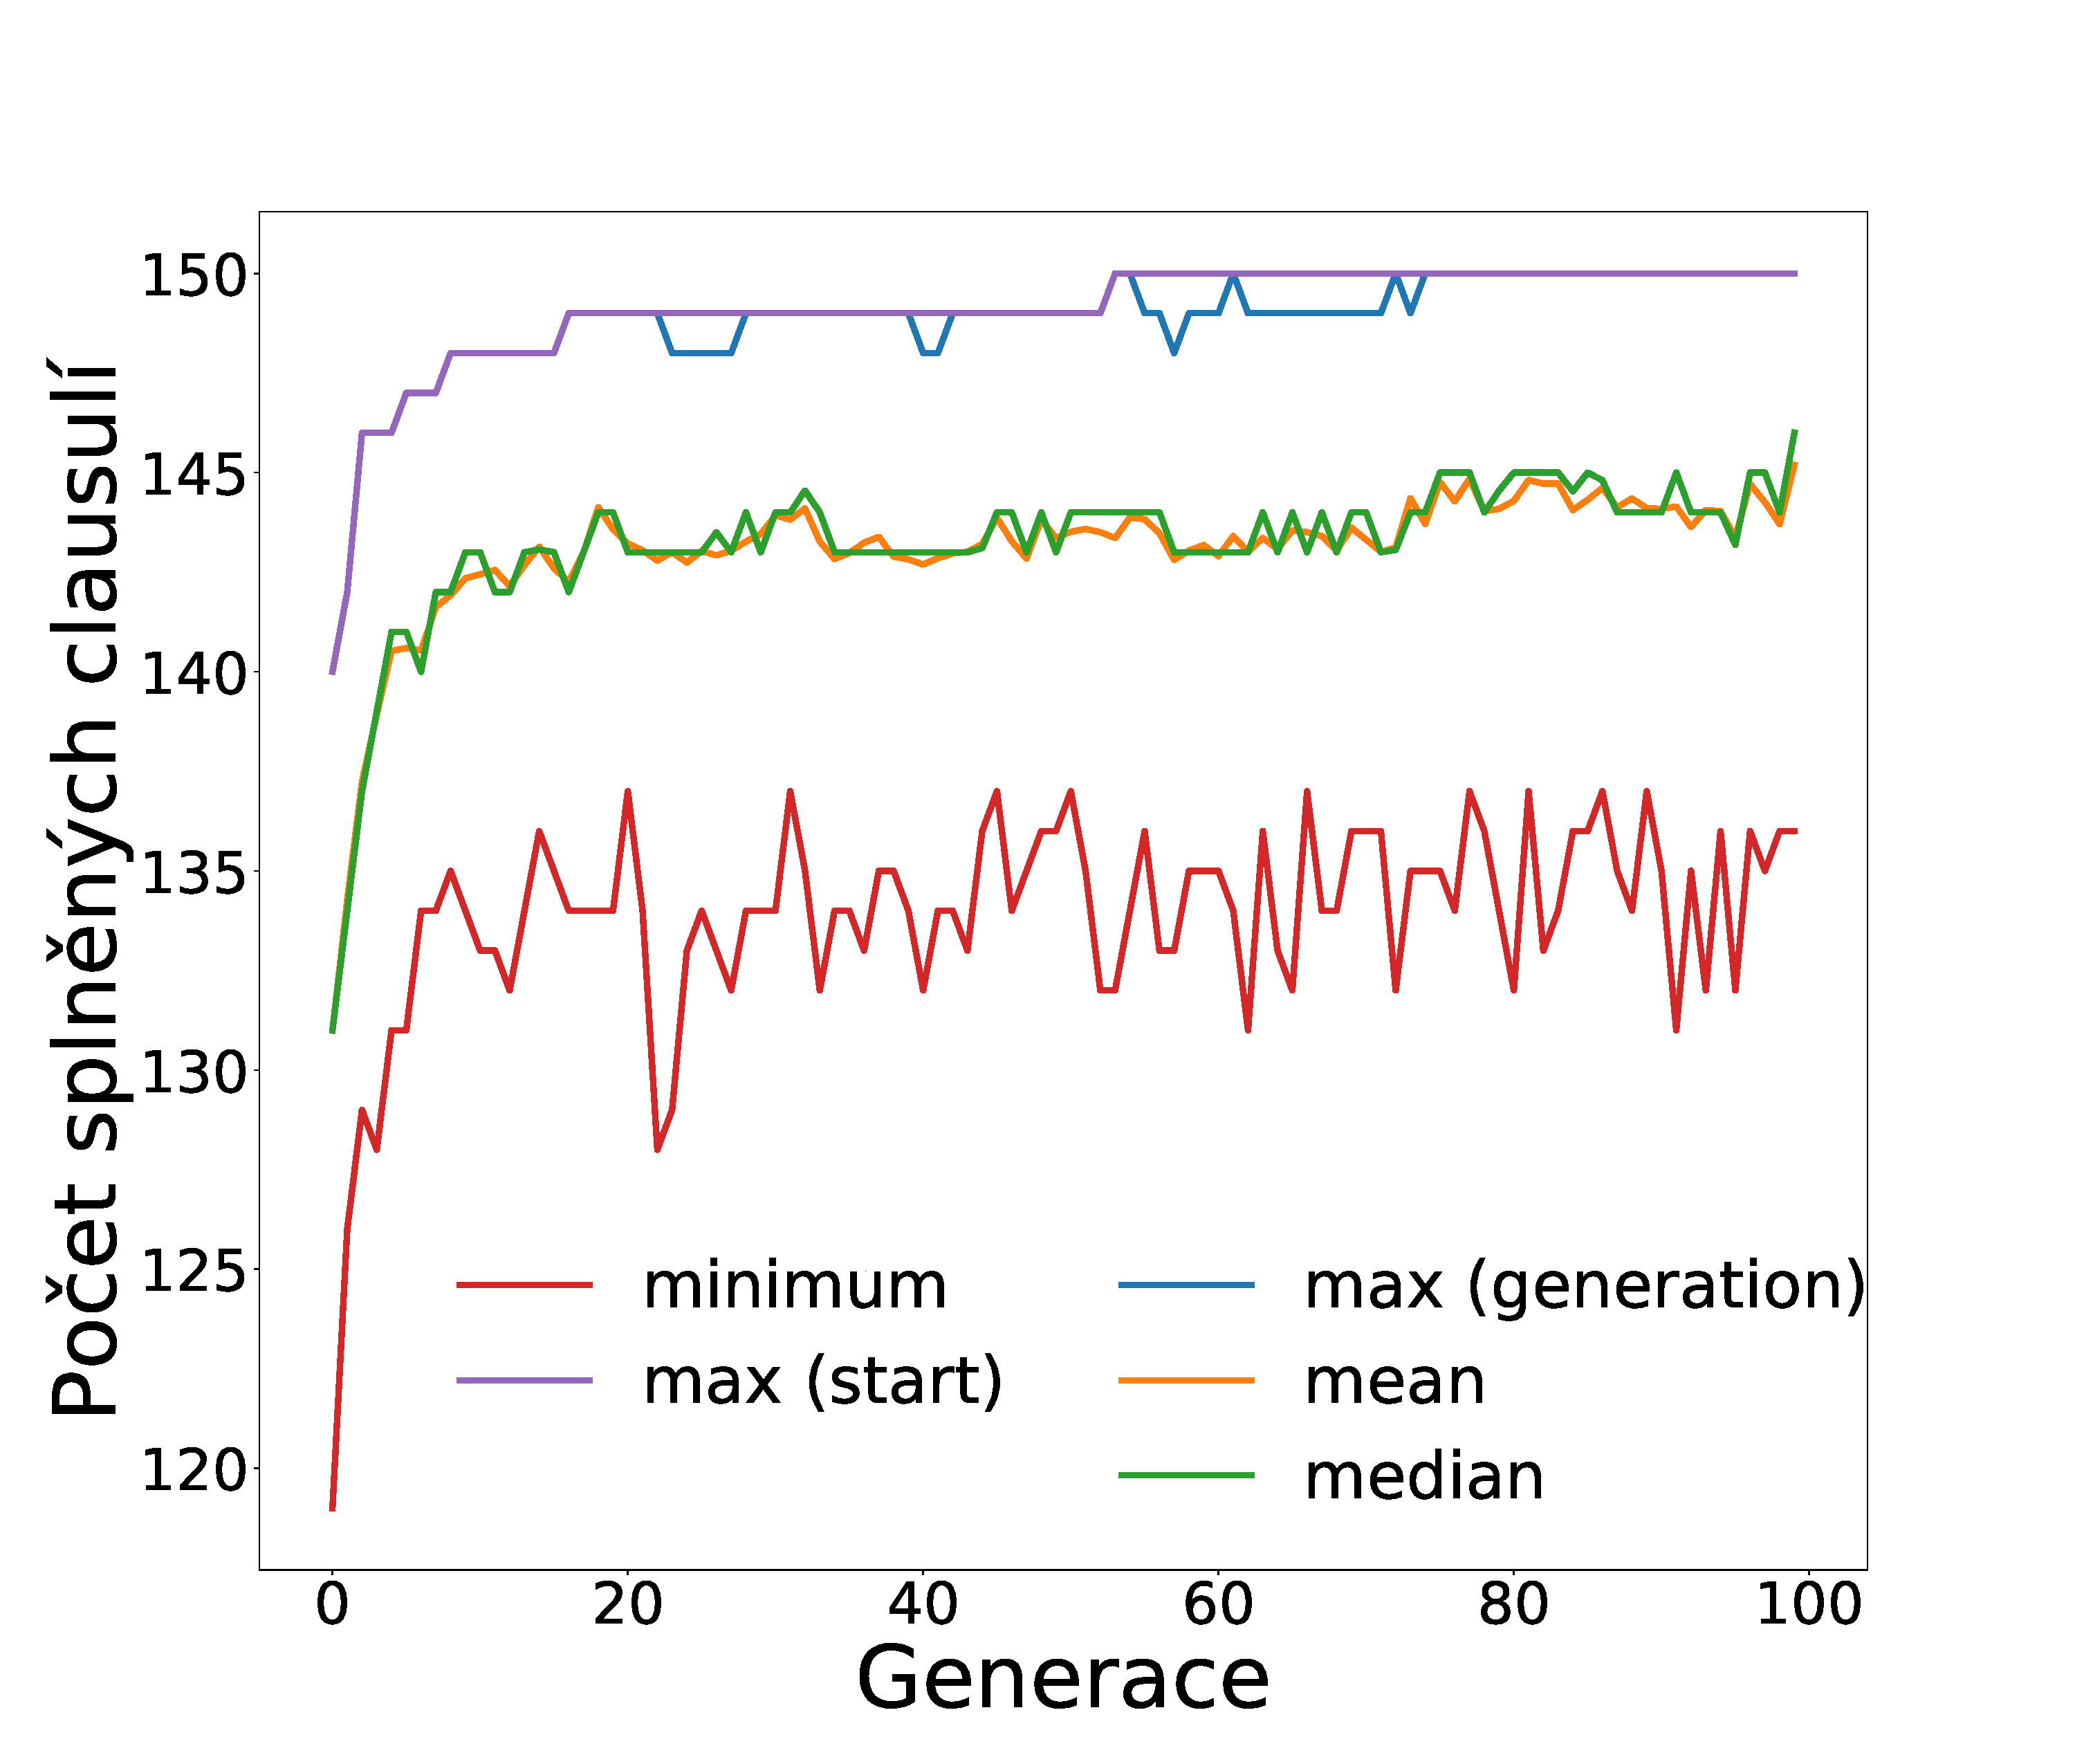
\includegraphics[width=\textwidth]{img/1c.pdf} 
    \end{minipage}
    \begin{minipage}[c]{0.42\textwidth}
        \centering 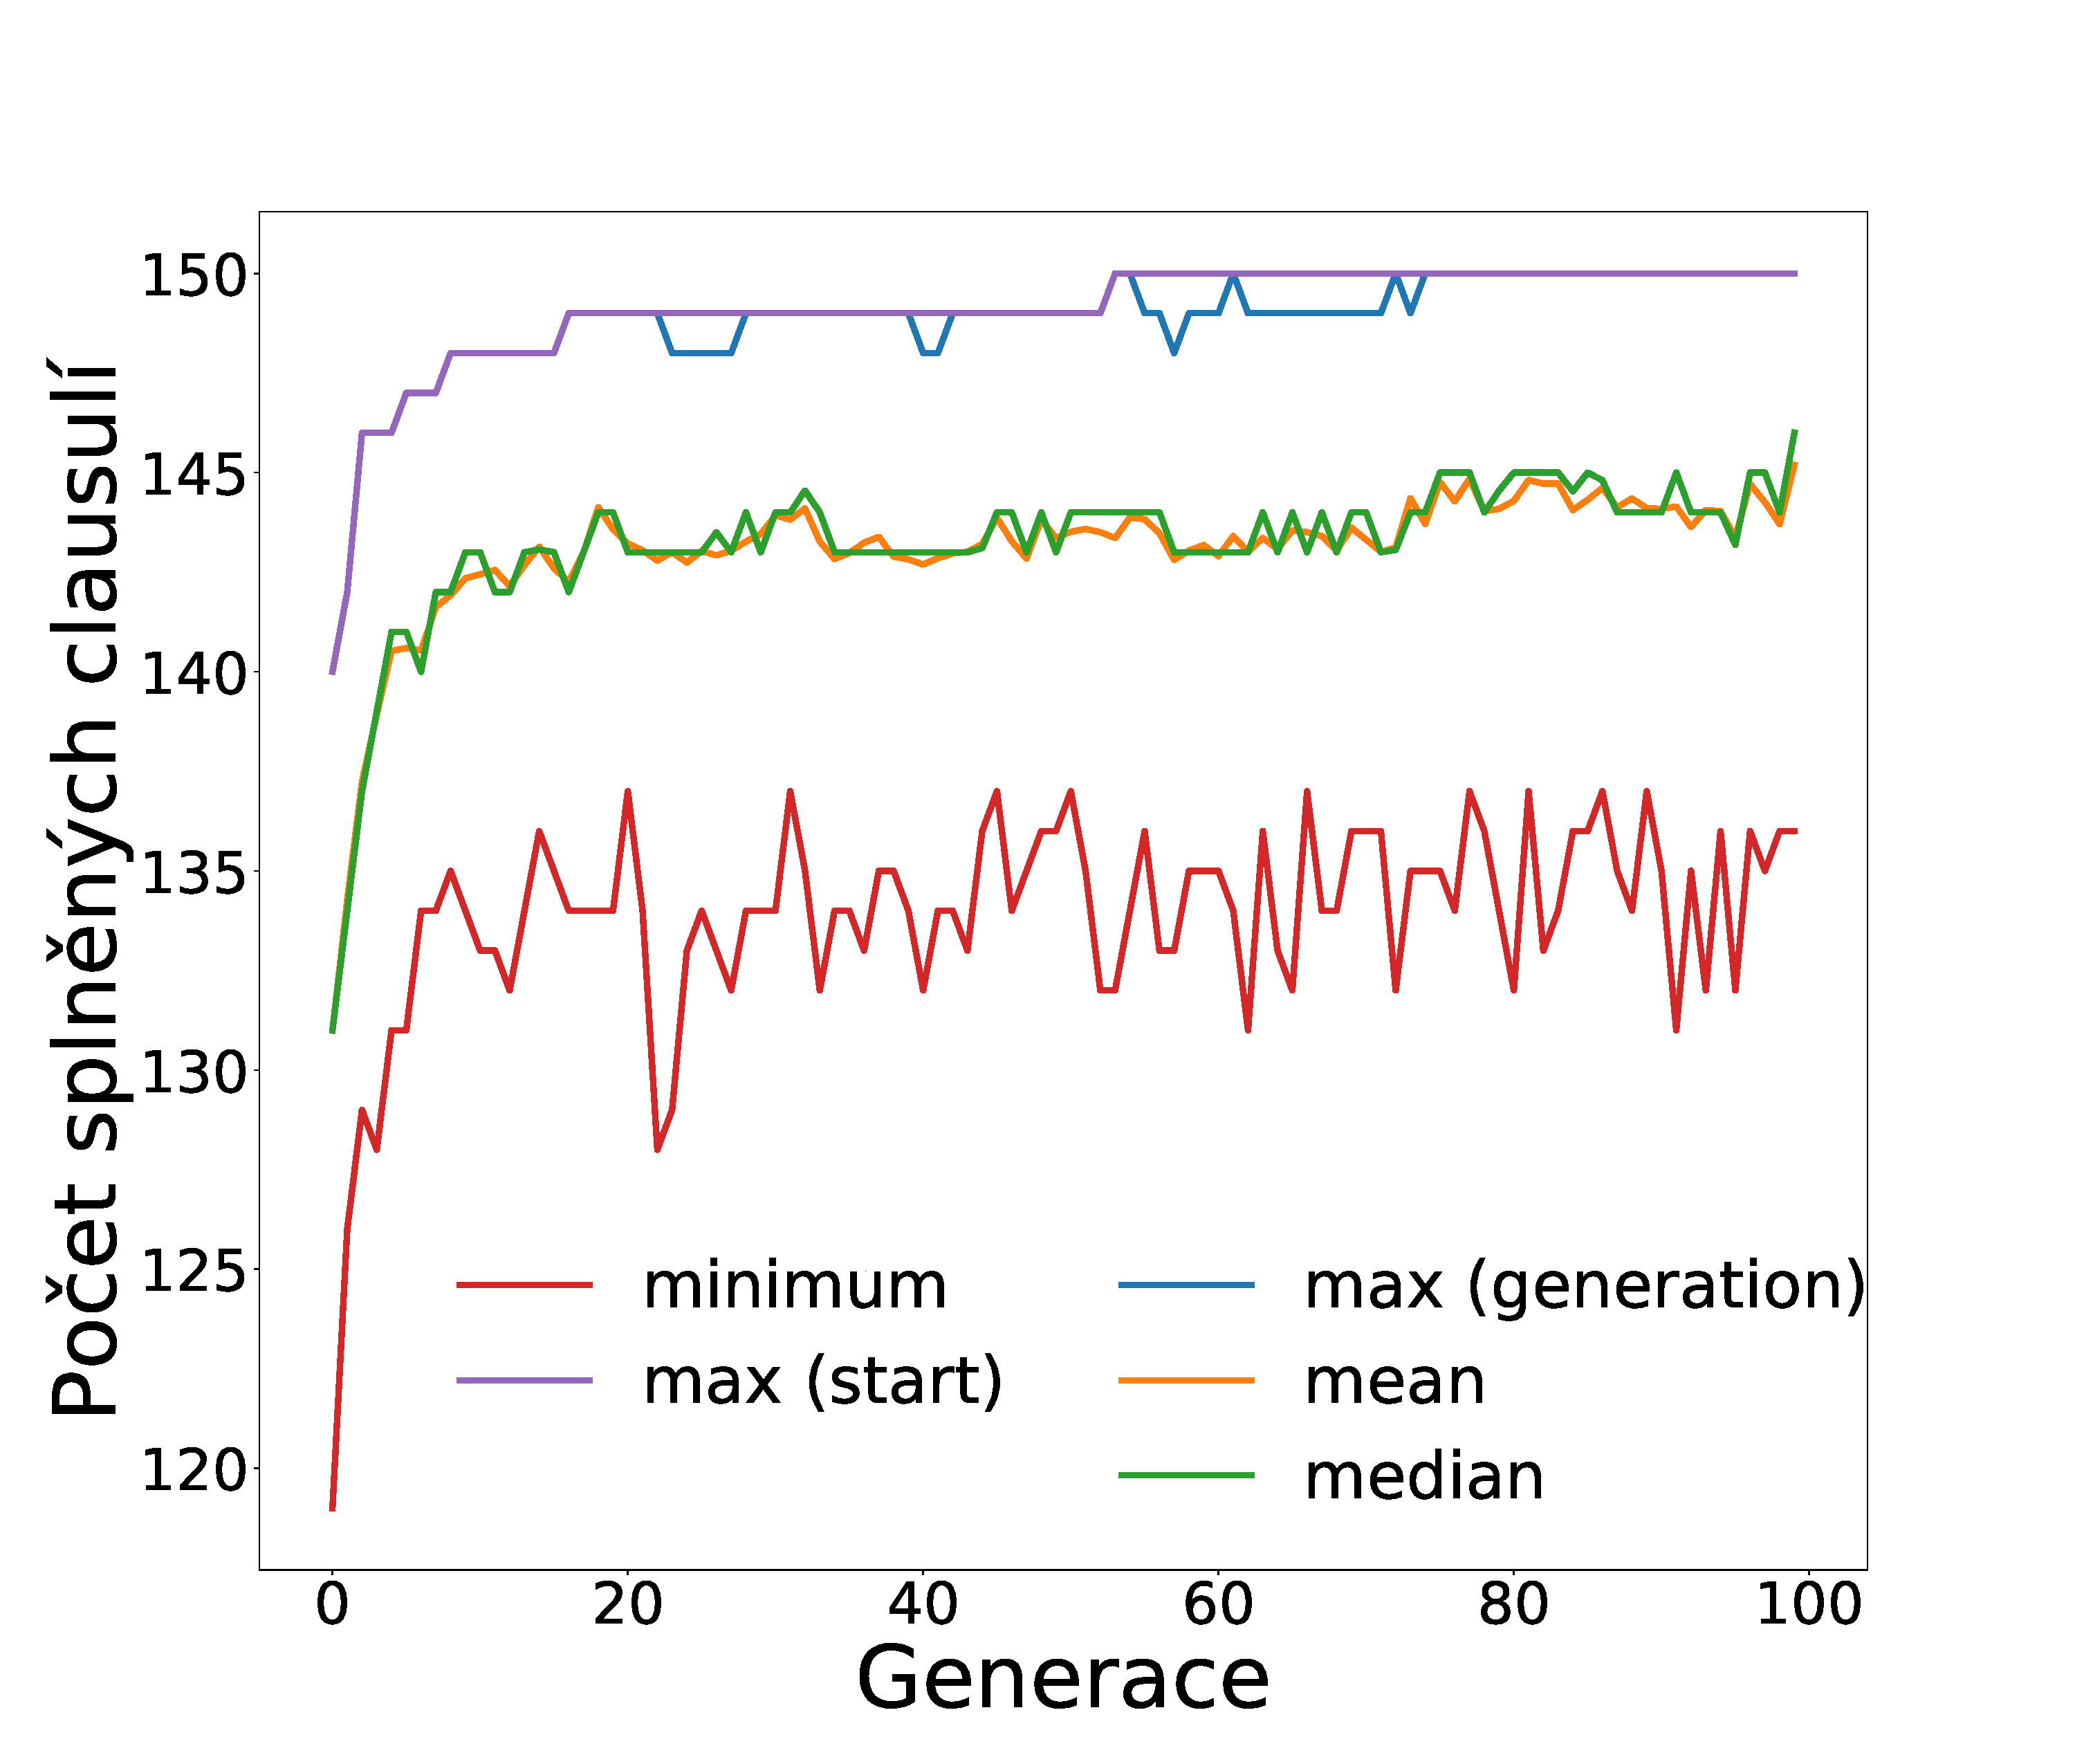
\includegraphics[width=\textwidth]{img/1c.pdf} 
    \end{minipage}
    \\
   \caption{Na levém grafu je závislost relativní chyby na počáteční teplotě. Na pravém grafu je závislost výpočetního času na počáteční teplotě}\label{fig:GZNT}
\end{figure} 

\begin{figure}
	\centering
    \begin{minipage}[c]{0.325\textwidth}
        \centering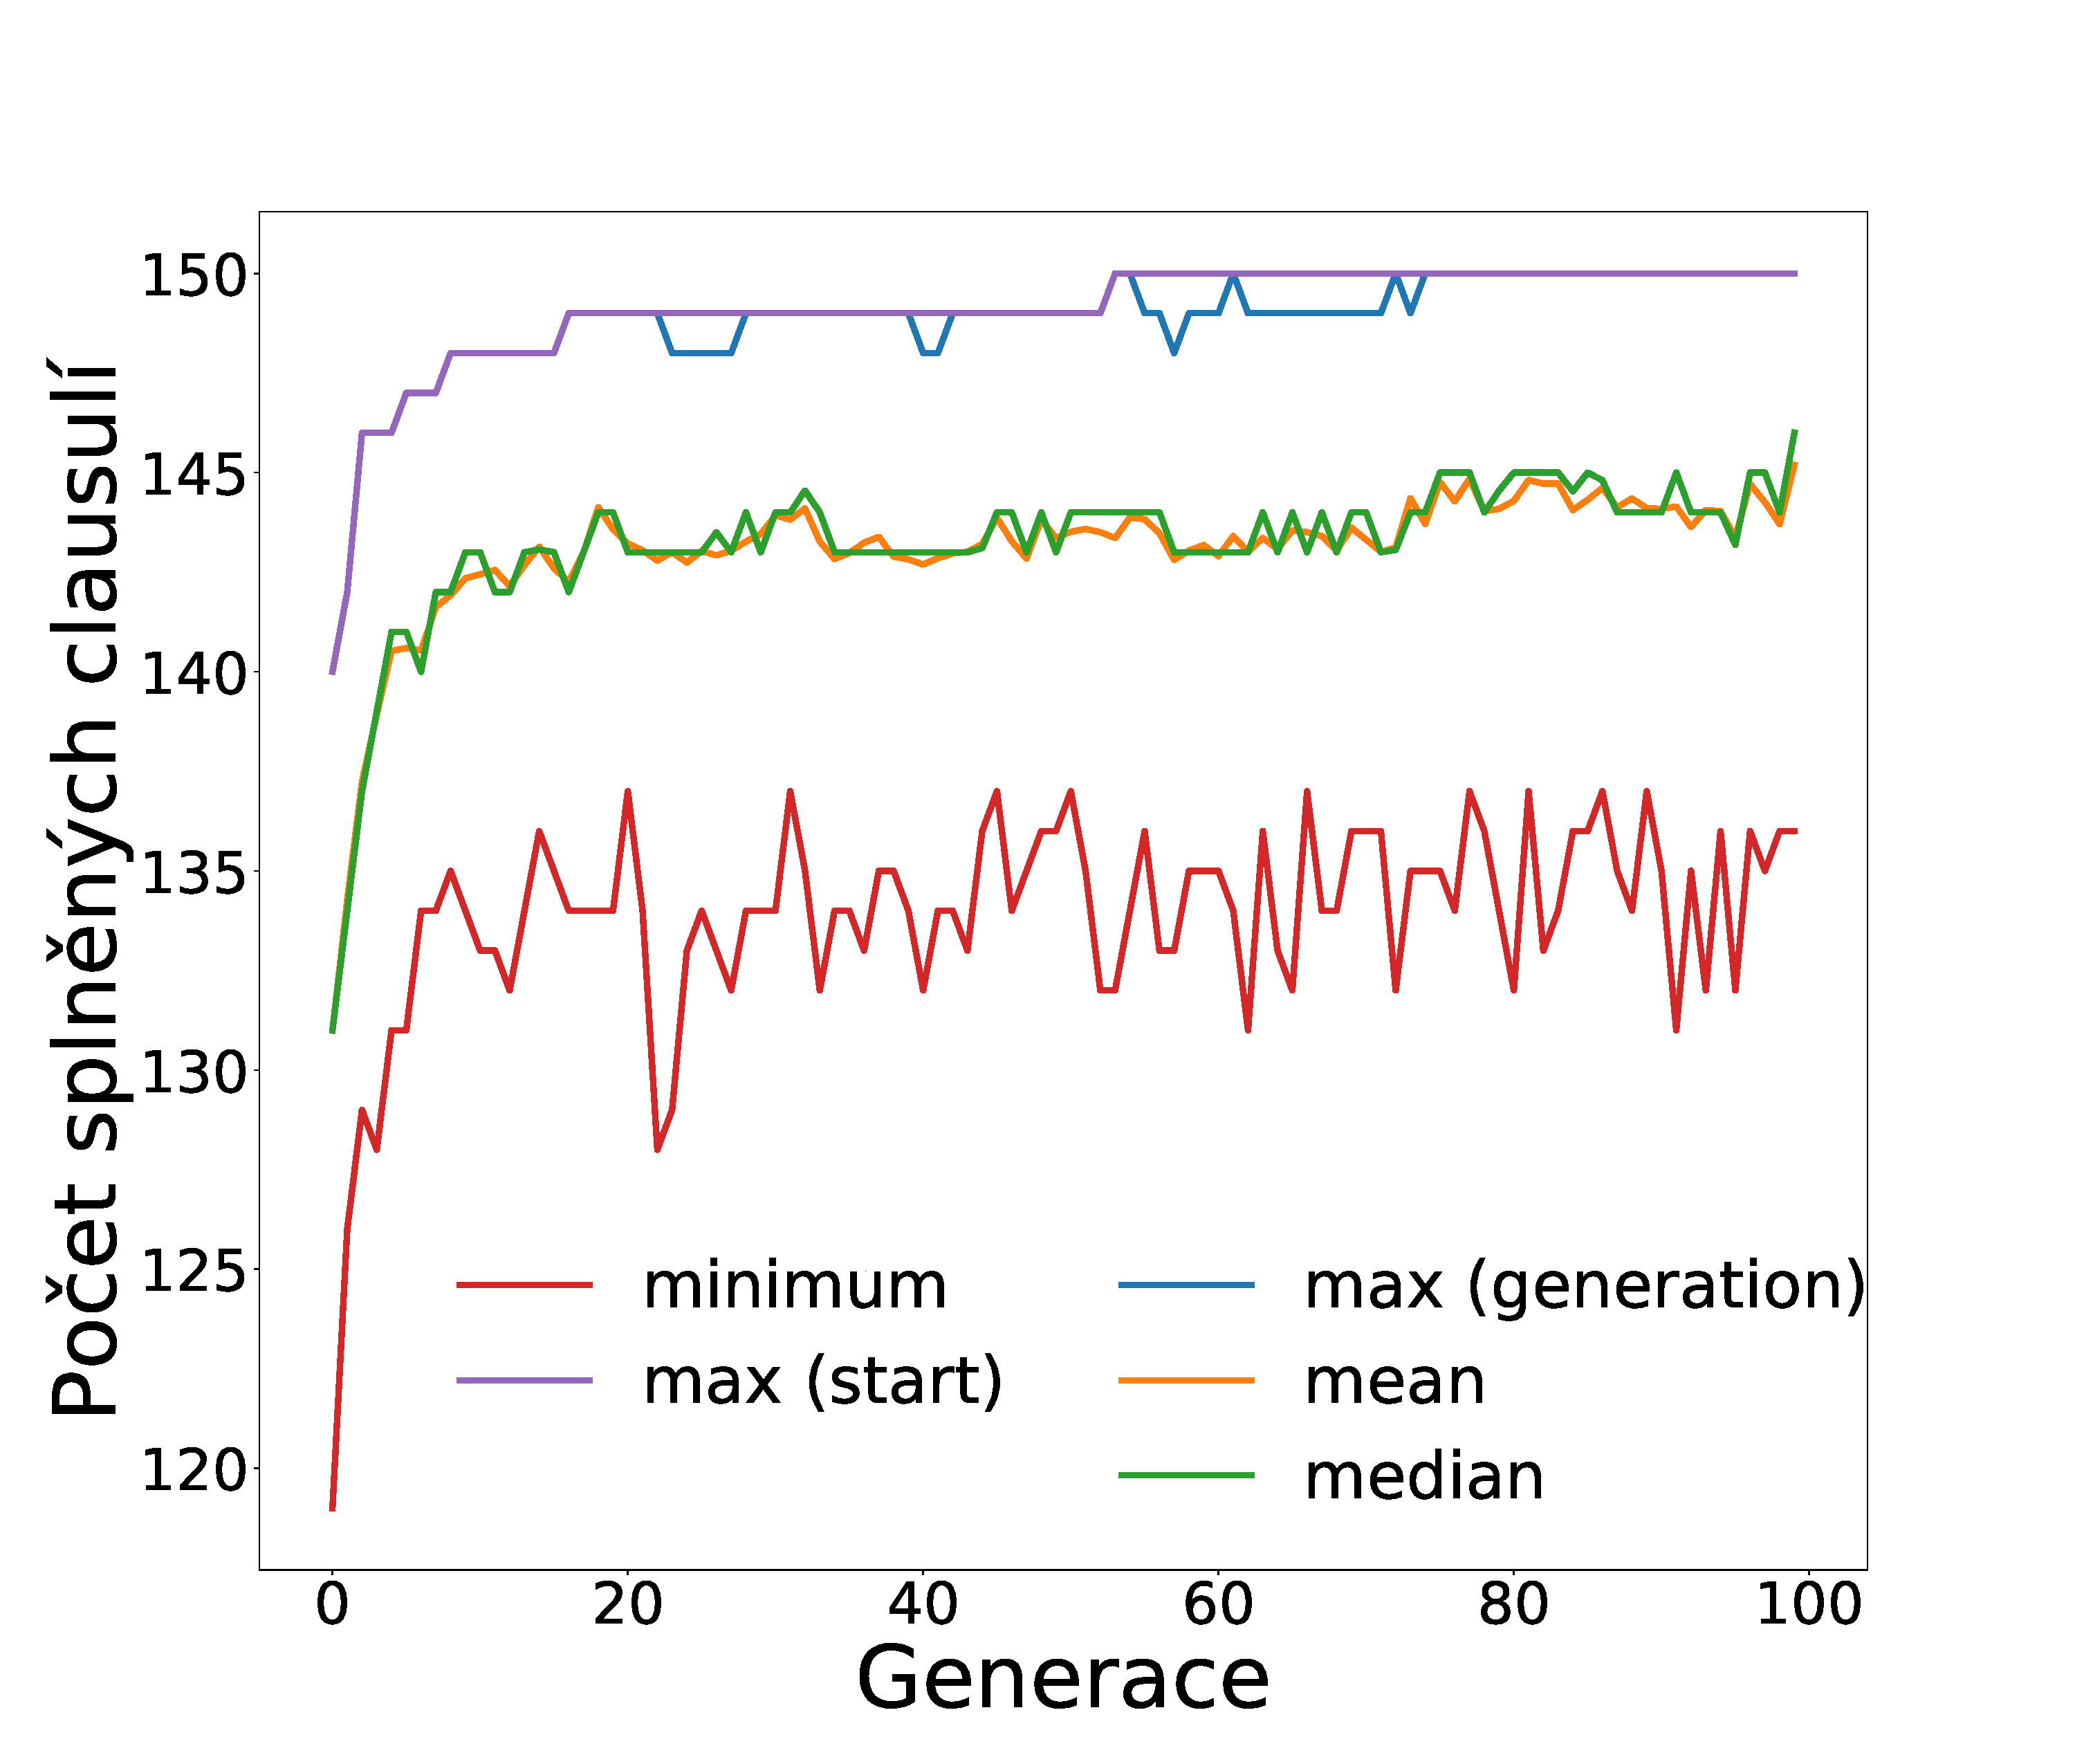
\includegraphics[width=\textwidth]{img/1c.pdf} 
    \end{minipage}
    \begin{minipage}[c]{0.325\textwidth}
        \centering 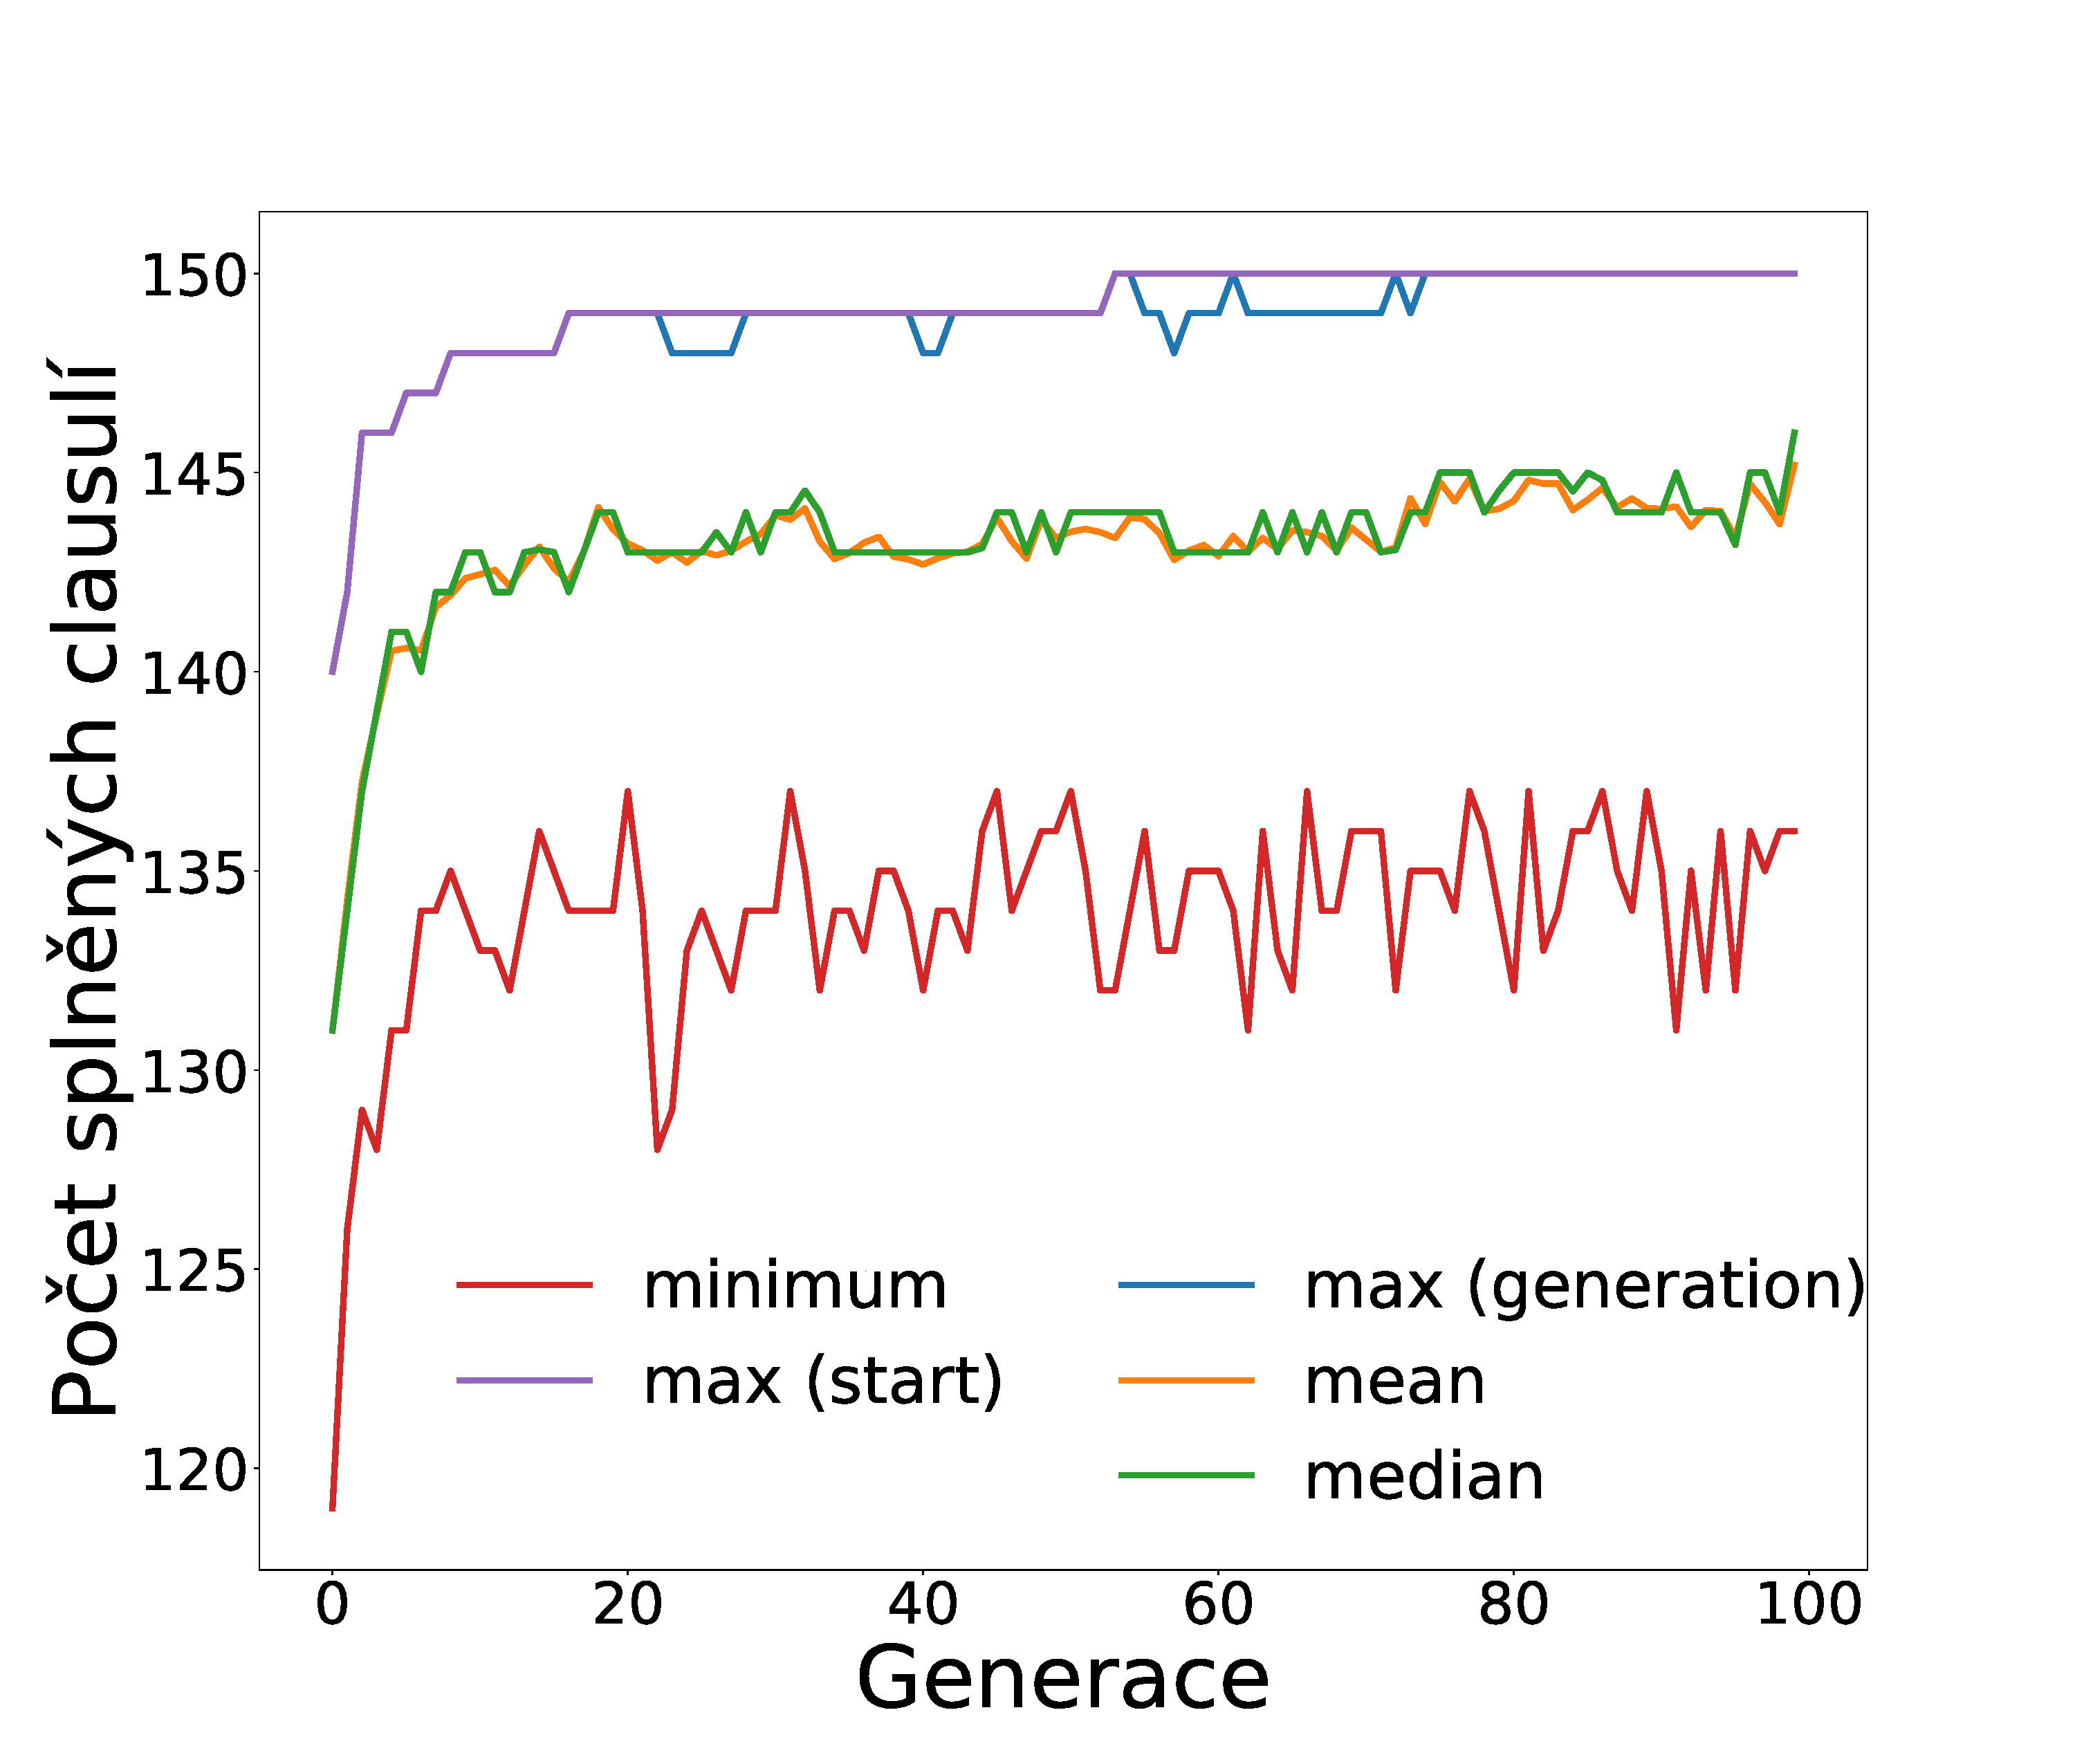
\includegraphics[width=\textwidth]{img/1c.pdf} 
    \end{minipage}
    \begin{minipage}[c]{0.325\textwidth}
        \centering 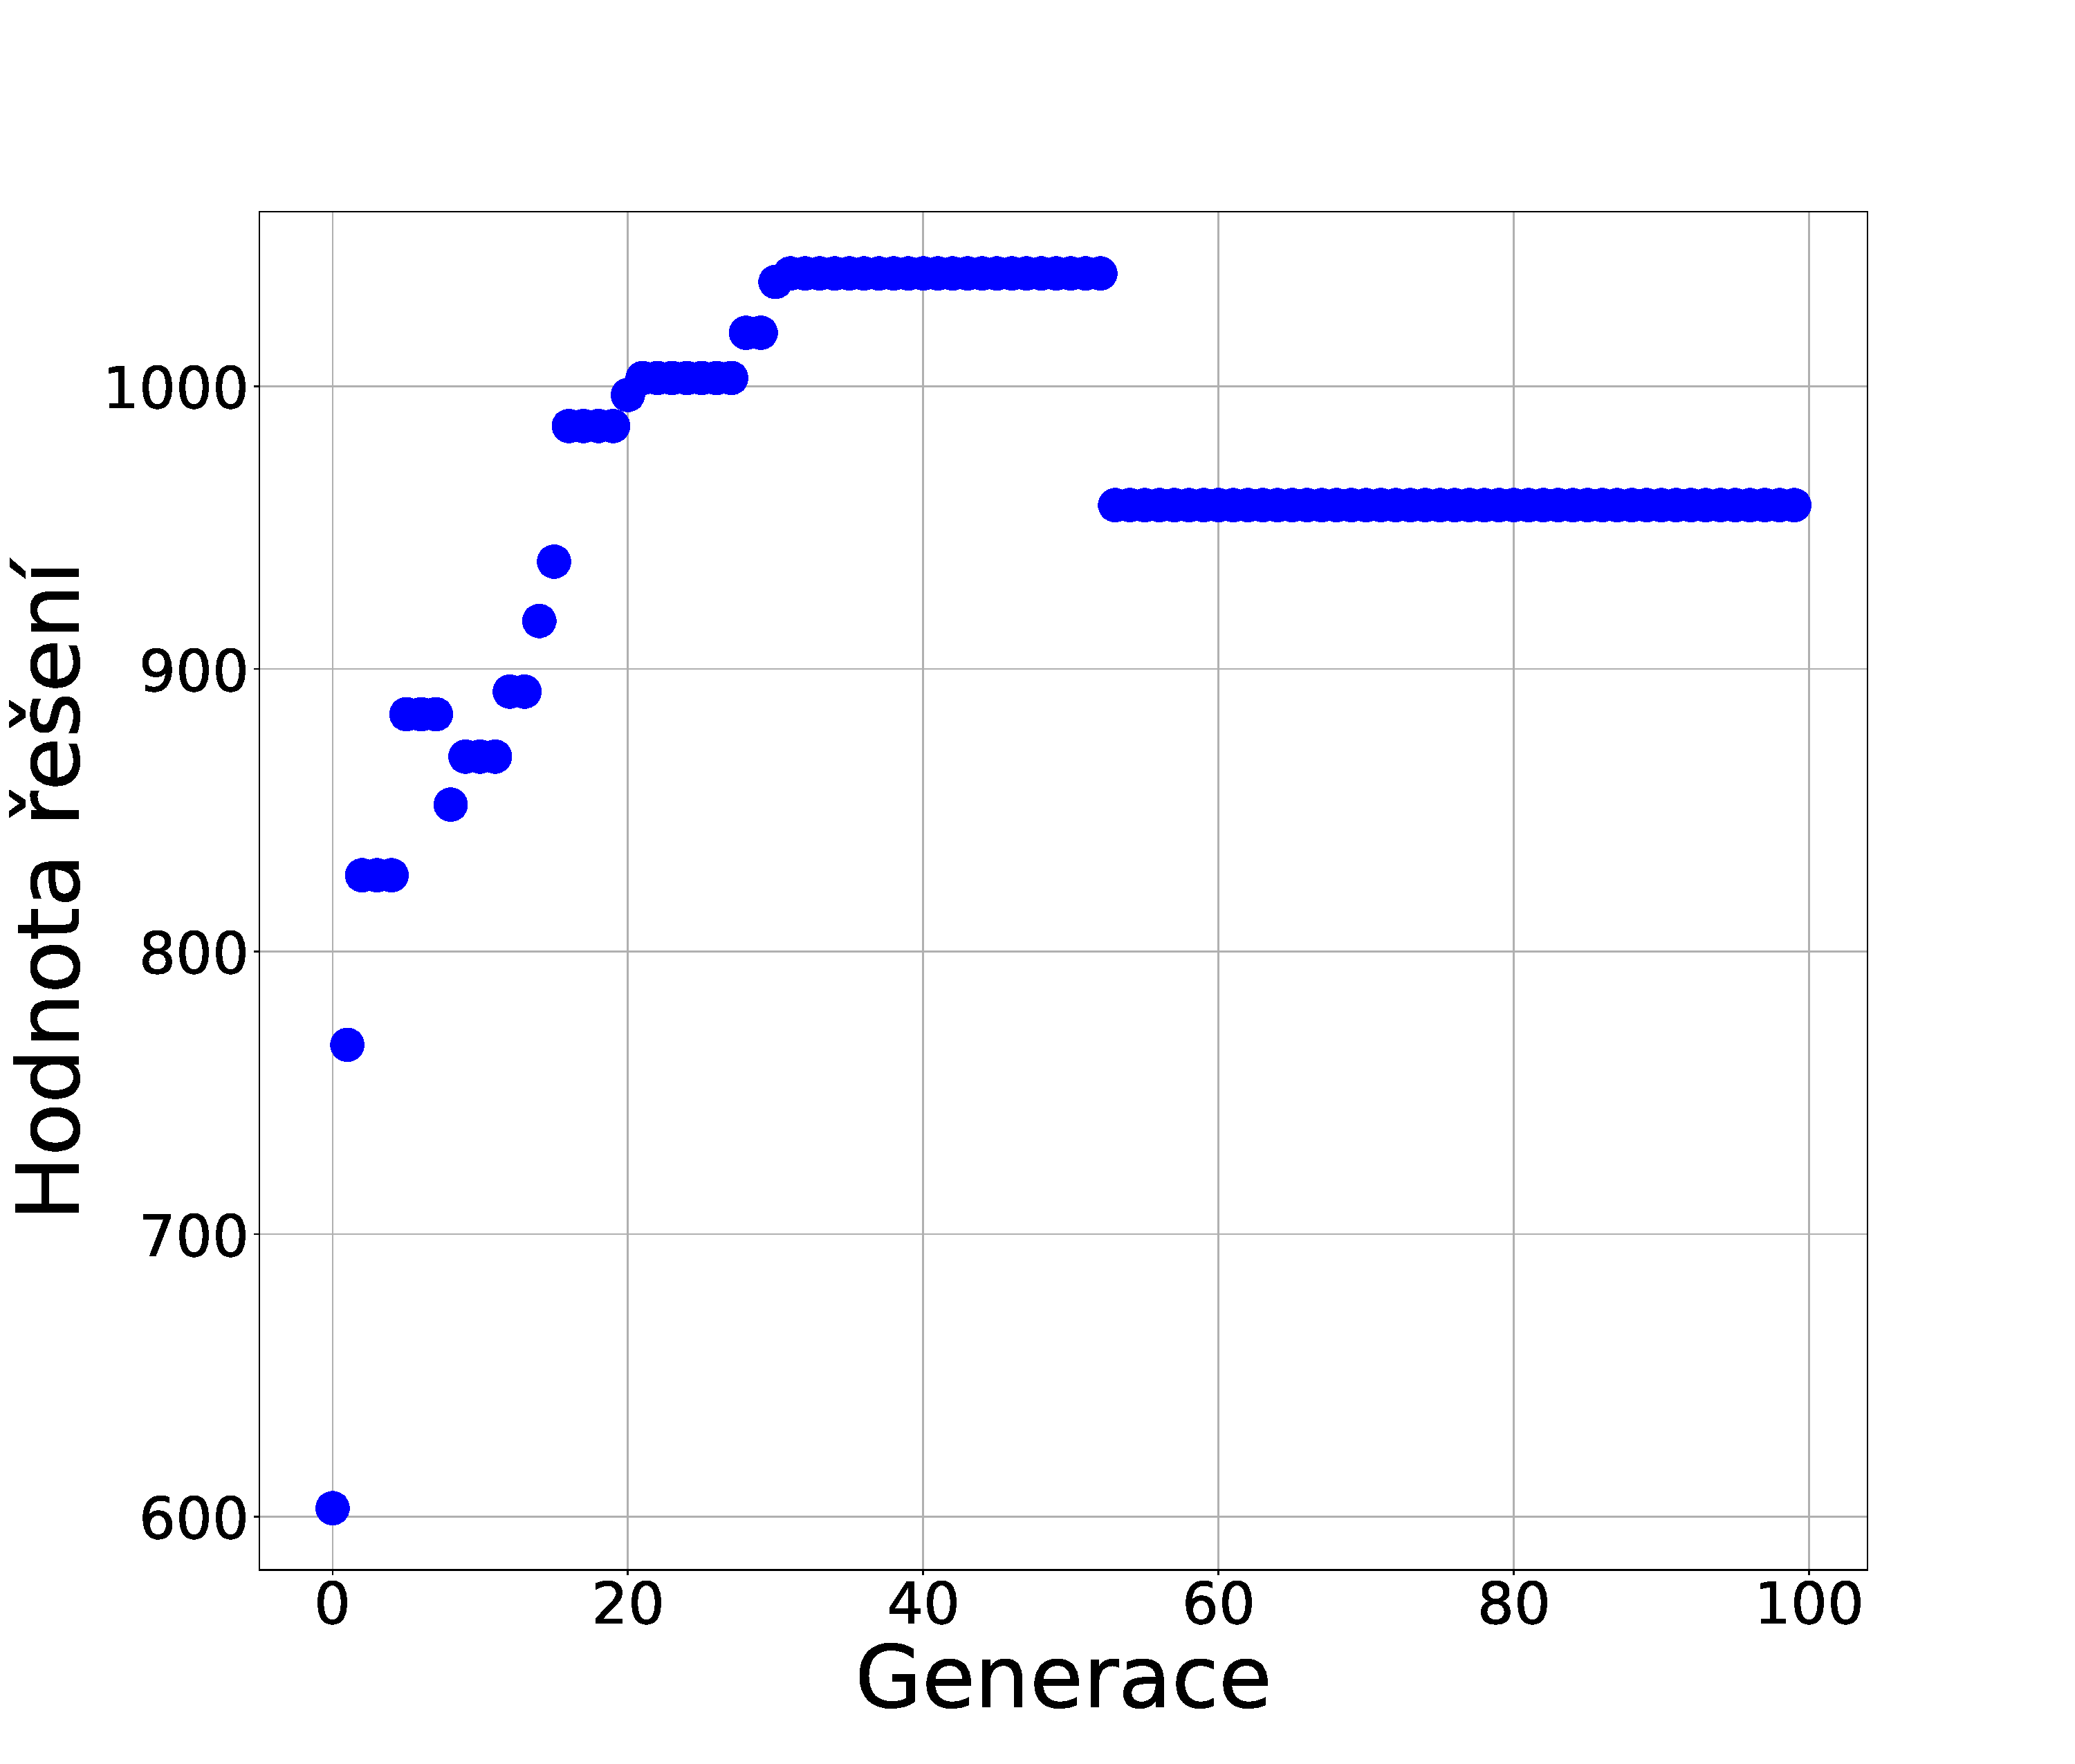
\includegraphics[width=\textwidth]{img/1w.pdf} 
    \end{minipage}
    \\
    \begin{minipage}[c]{0.49\textwidth}
        \centering 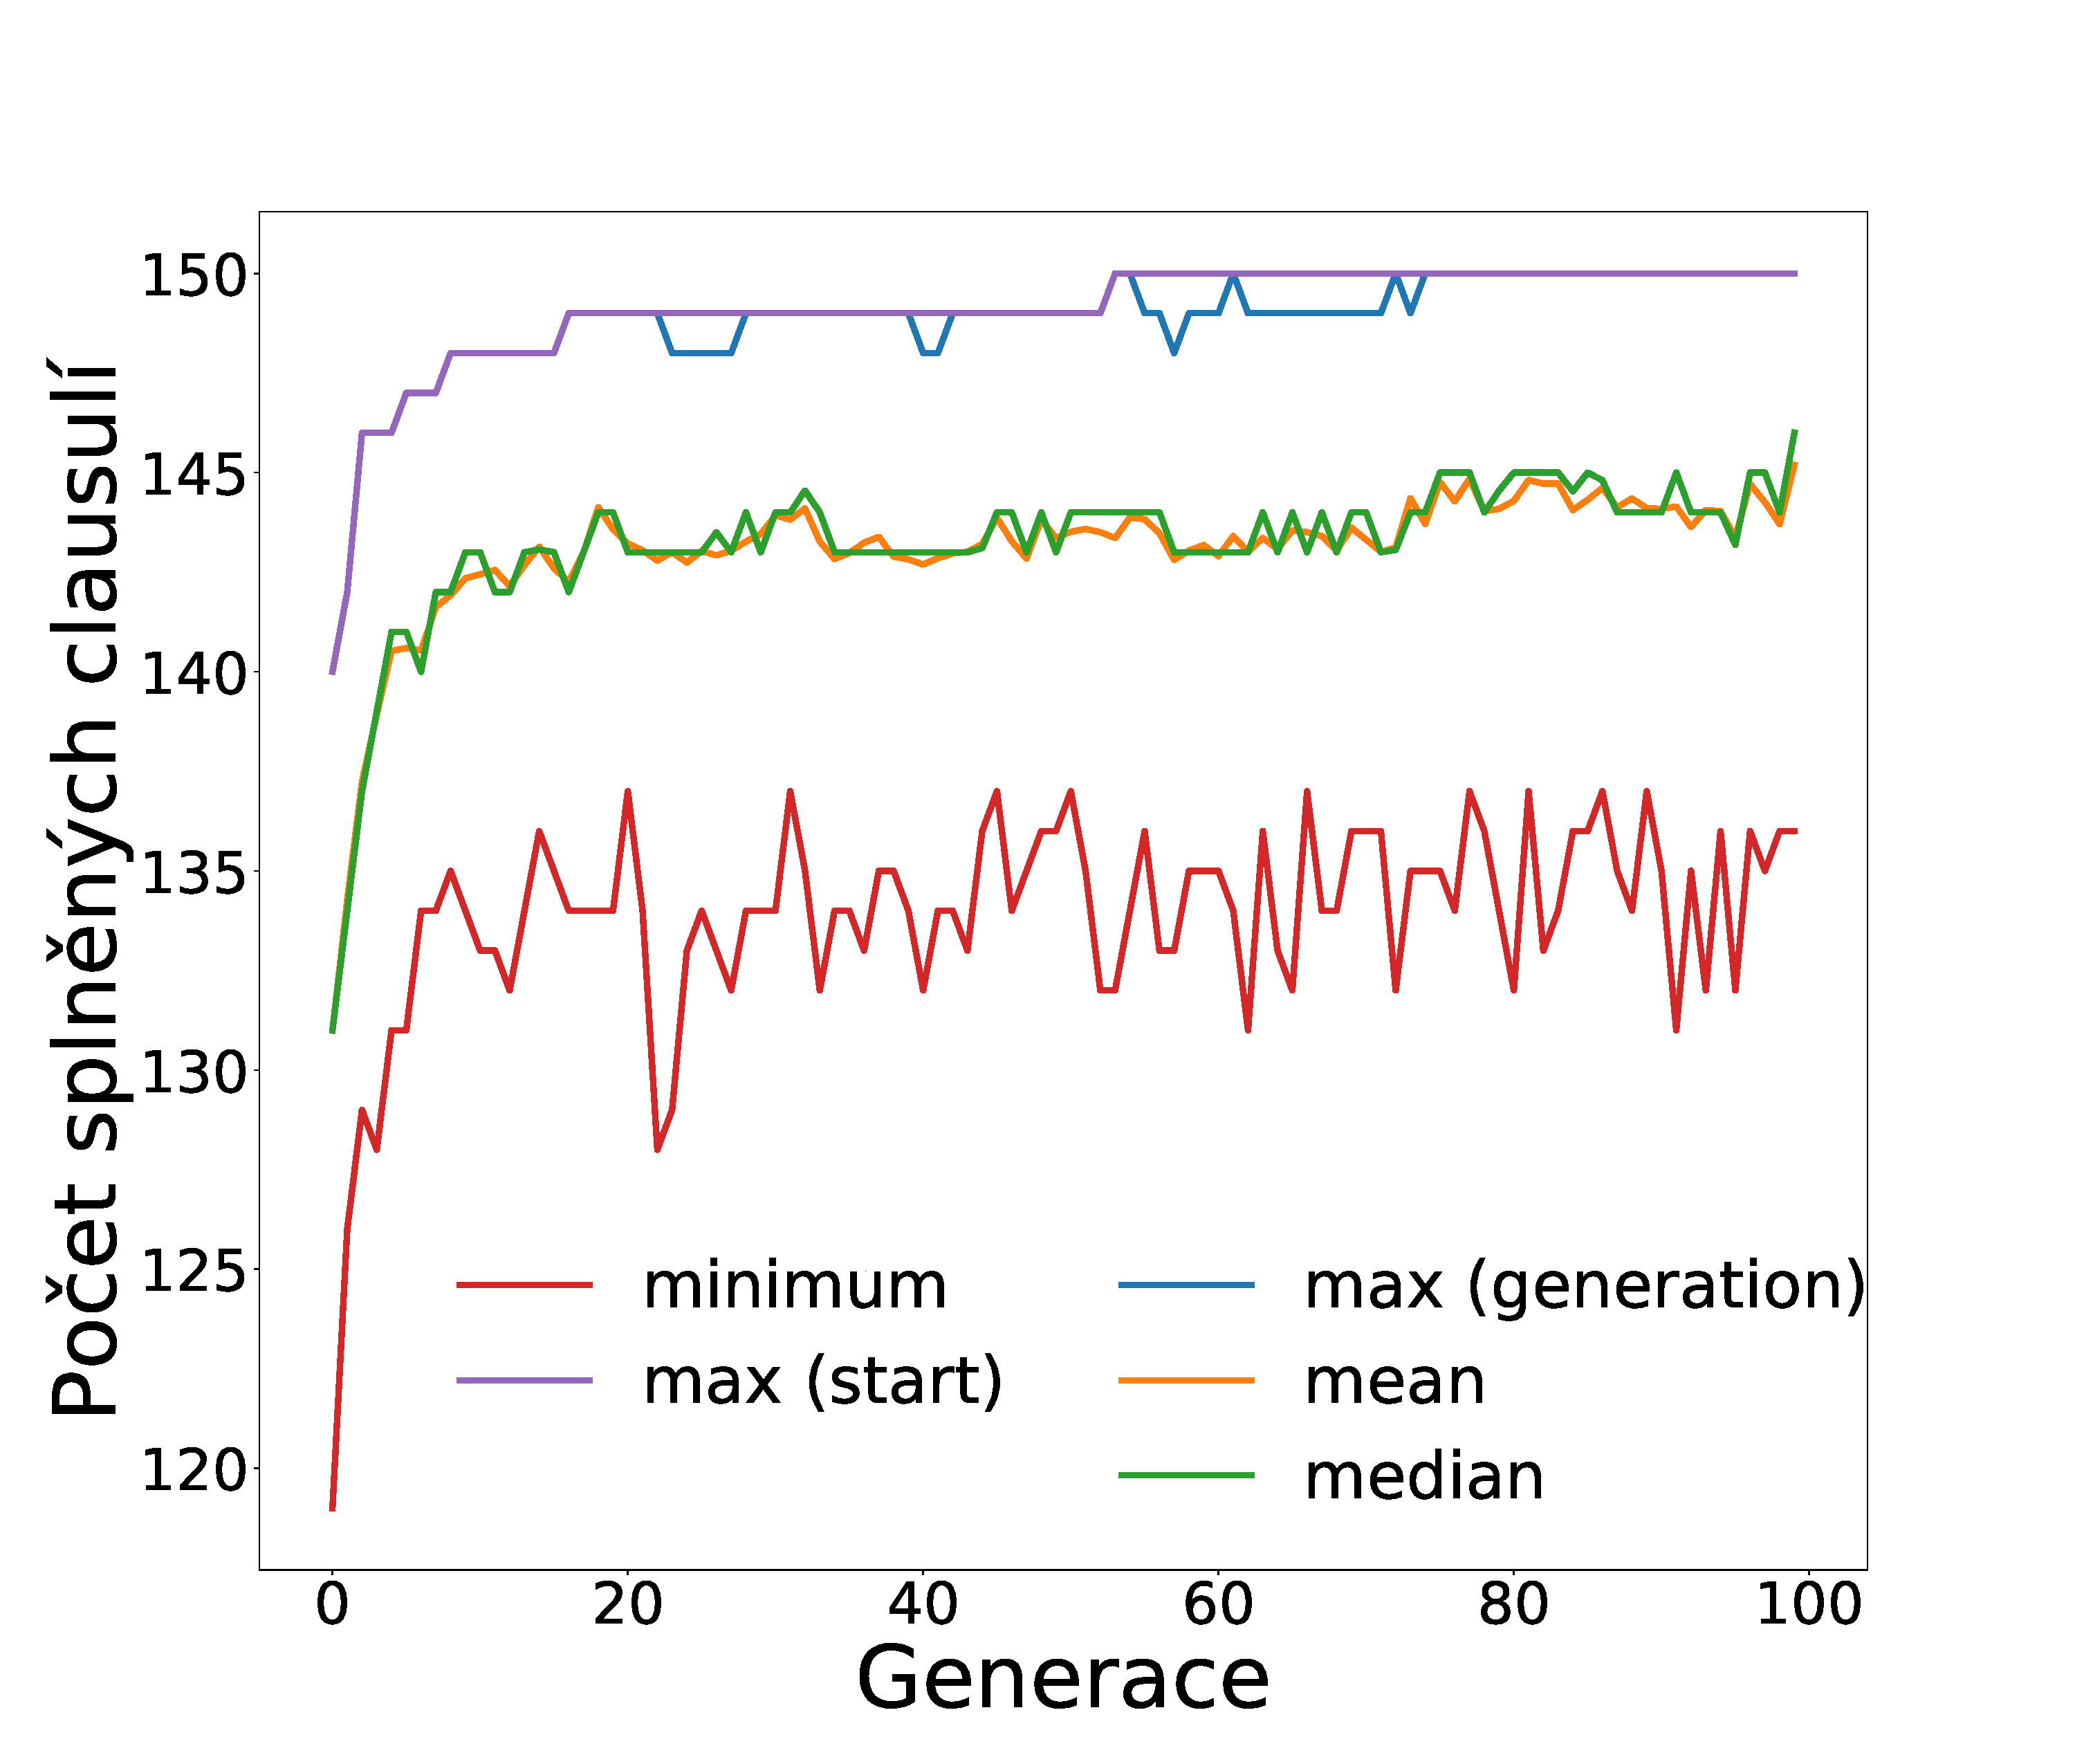
\includegraphics[width=\textwidth]{img/1c.pdf} 
    \end{minipage}
    \begin{minipage}[c]{0.49\textwidth}
        \centering 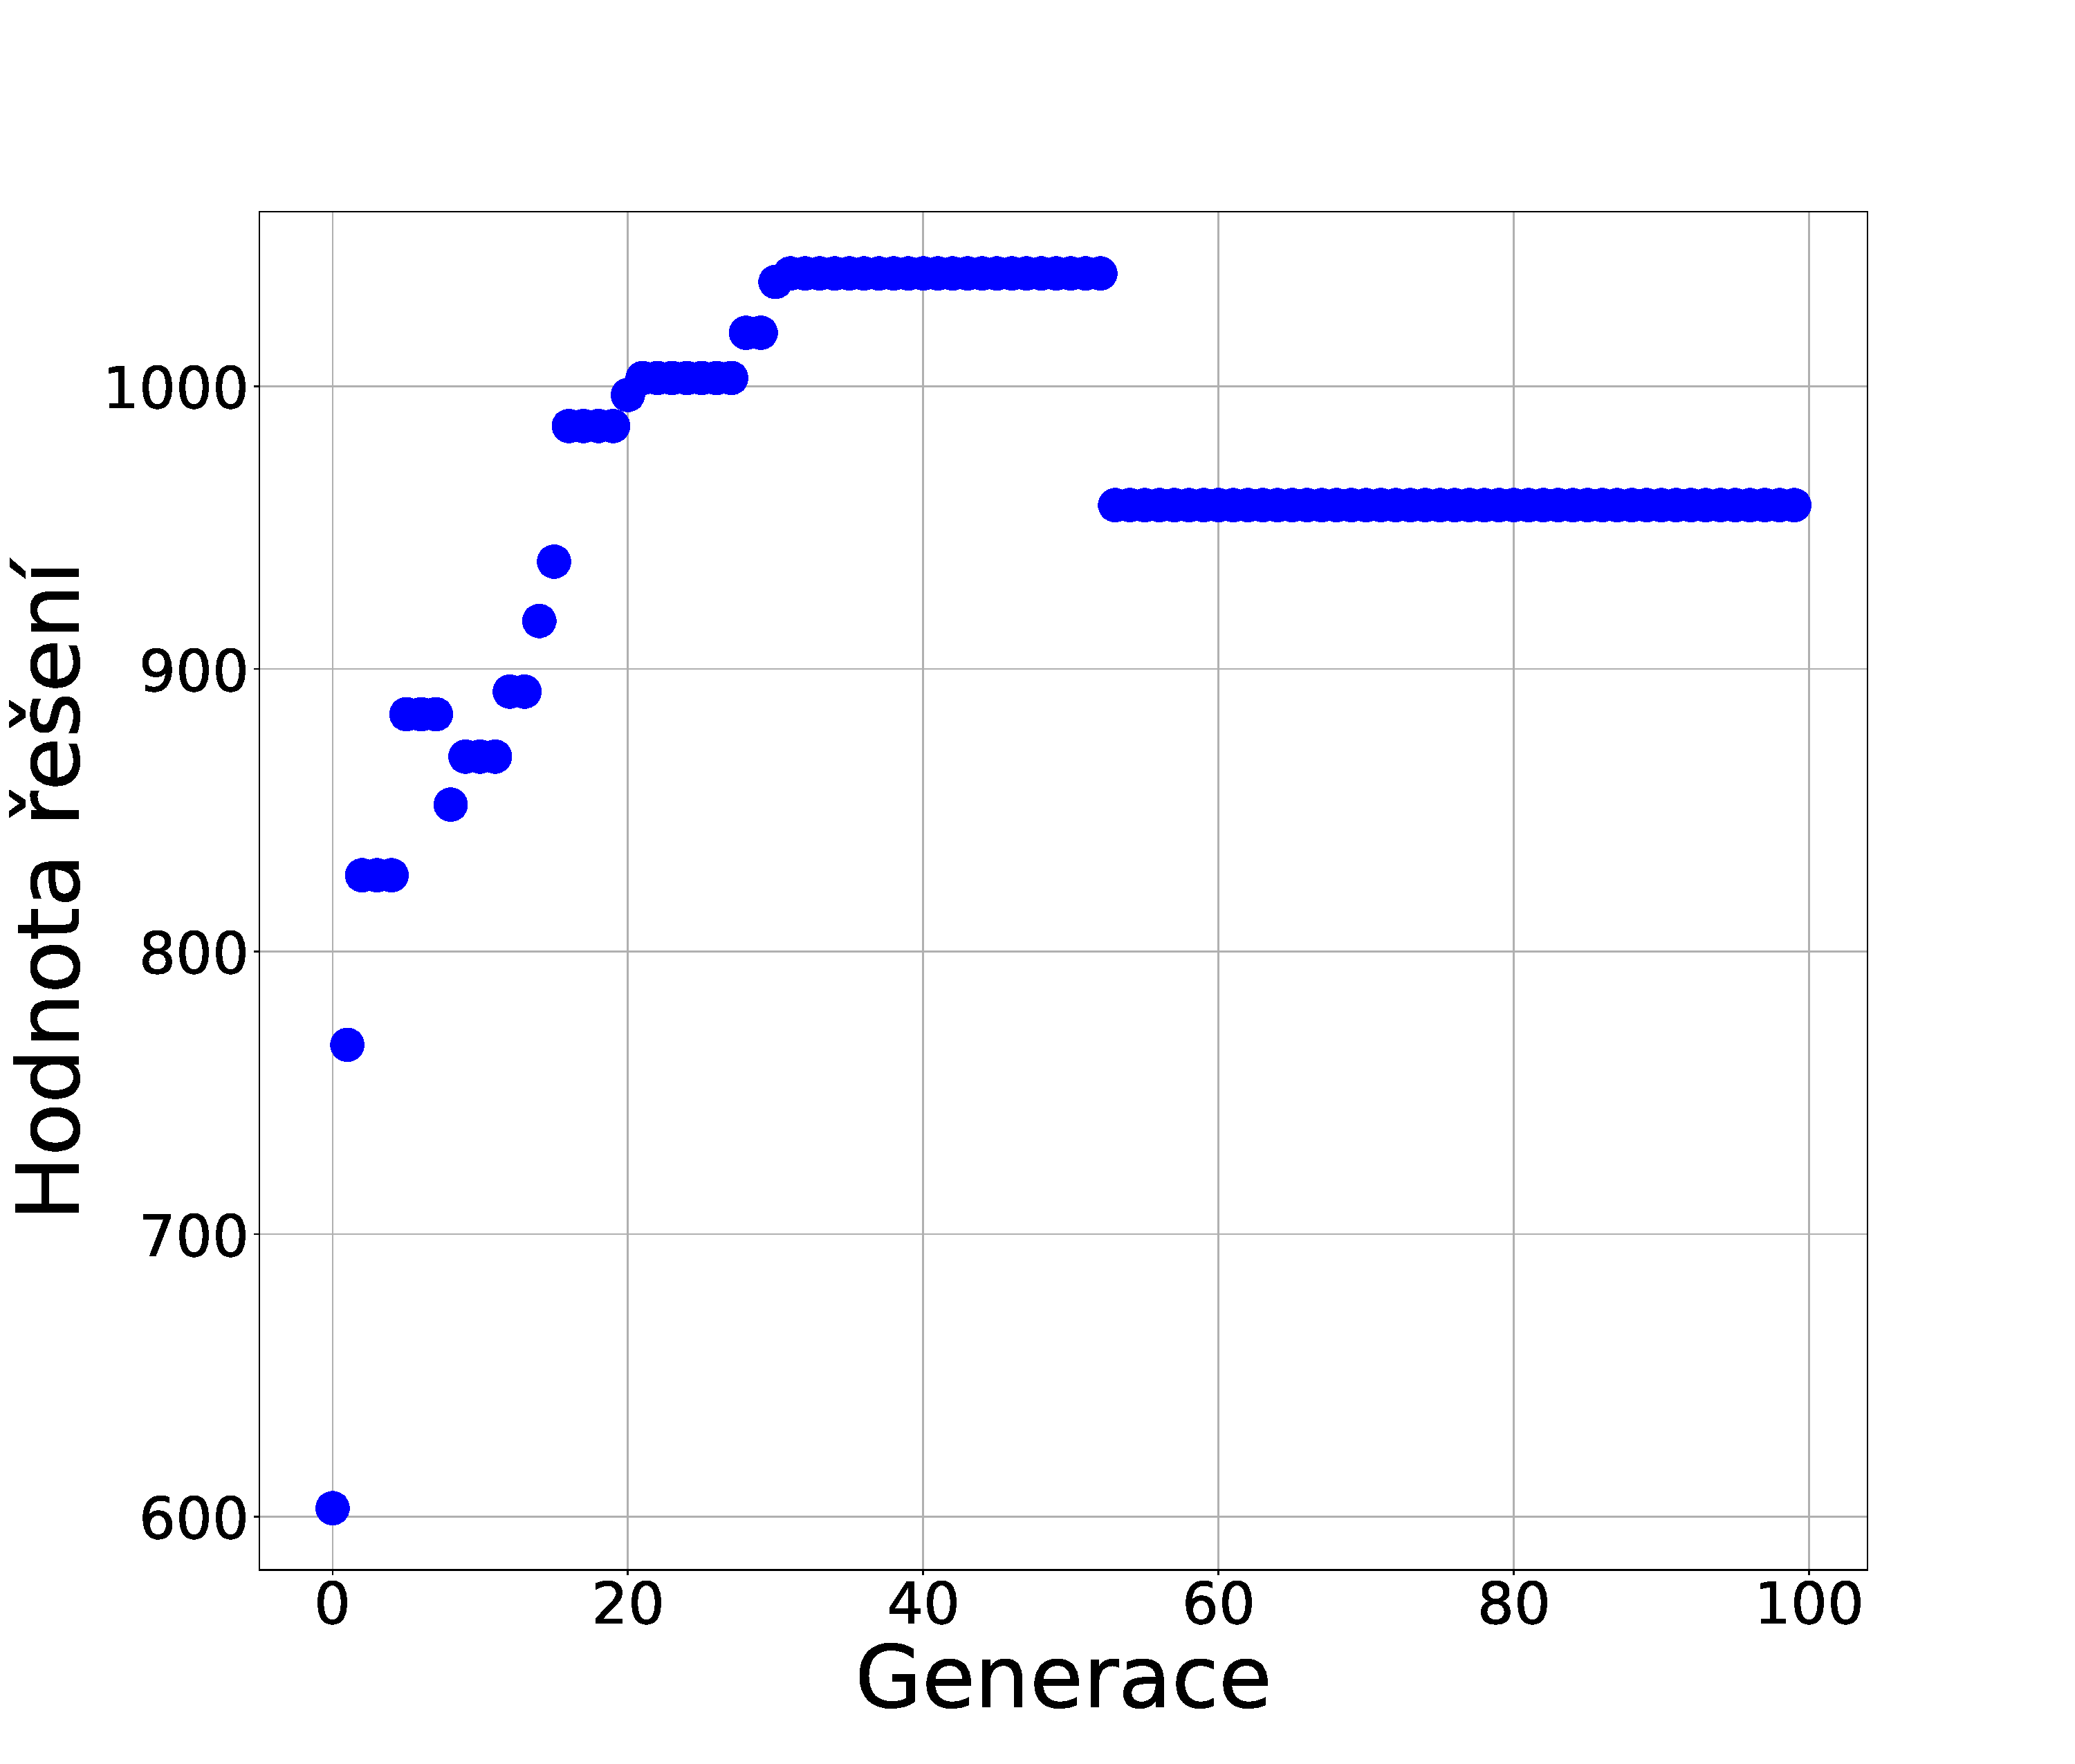
\includegraphics[width=\textwidth]{img/1w.pdf} 
    \end{minipage}
   \caption{Zde jsou uvedené grafy vývoje řešení pro vybrané hodnoty počtu iterácí na jedné teplotě. Konkrétně zleva pro hodnoty 30, 60, 120, 240, 300}\label{fig:GVPT}
\end{figure} 

 
\begin{figure}
	\centering
    \begin{minipage}[c]{0.42\textwidth}
        \centering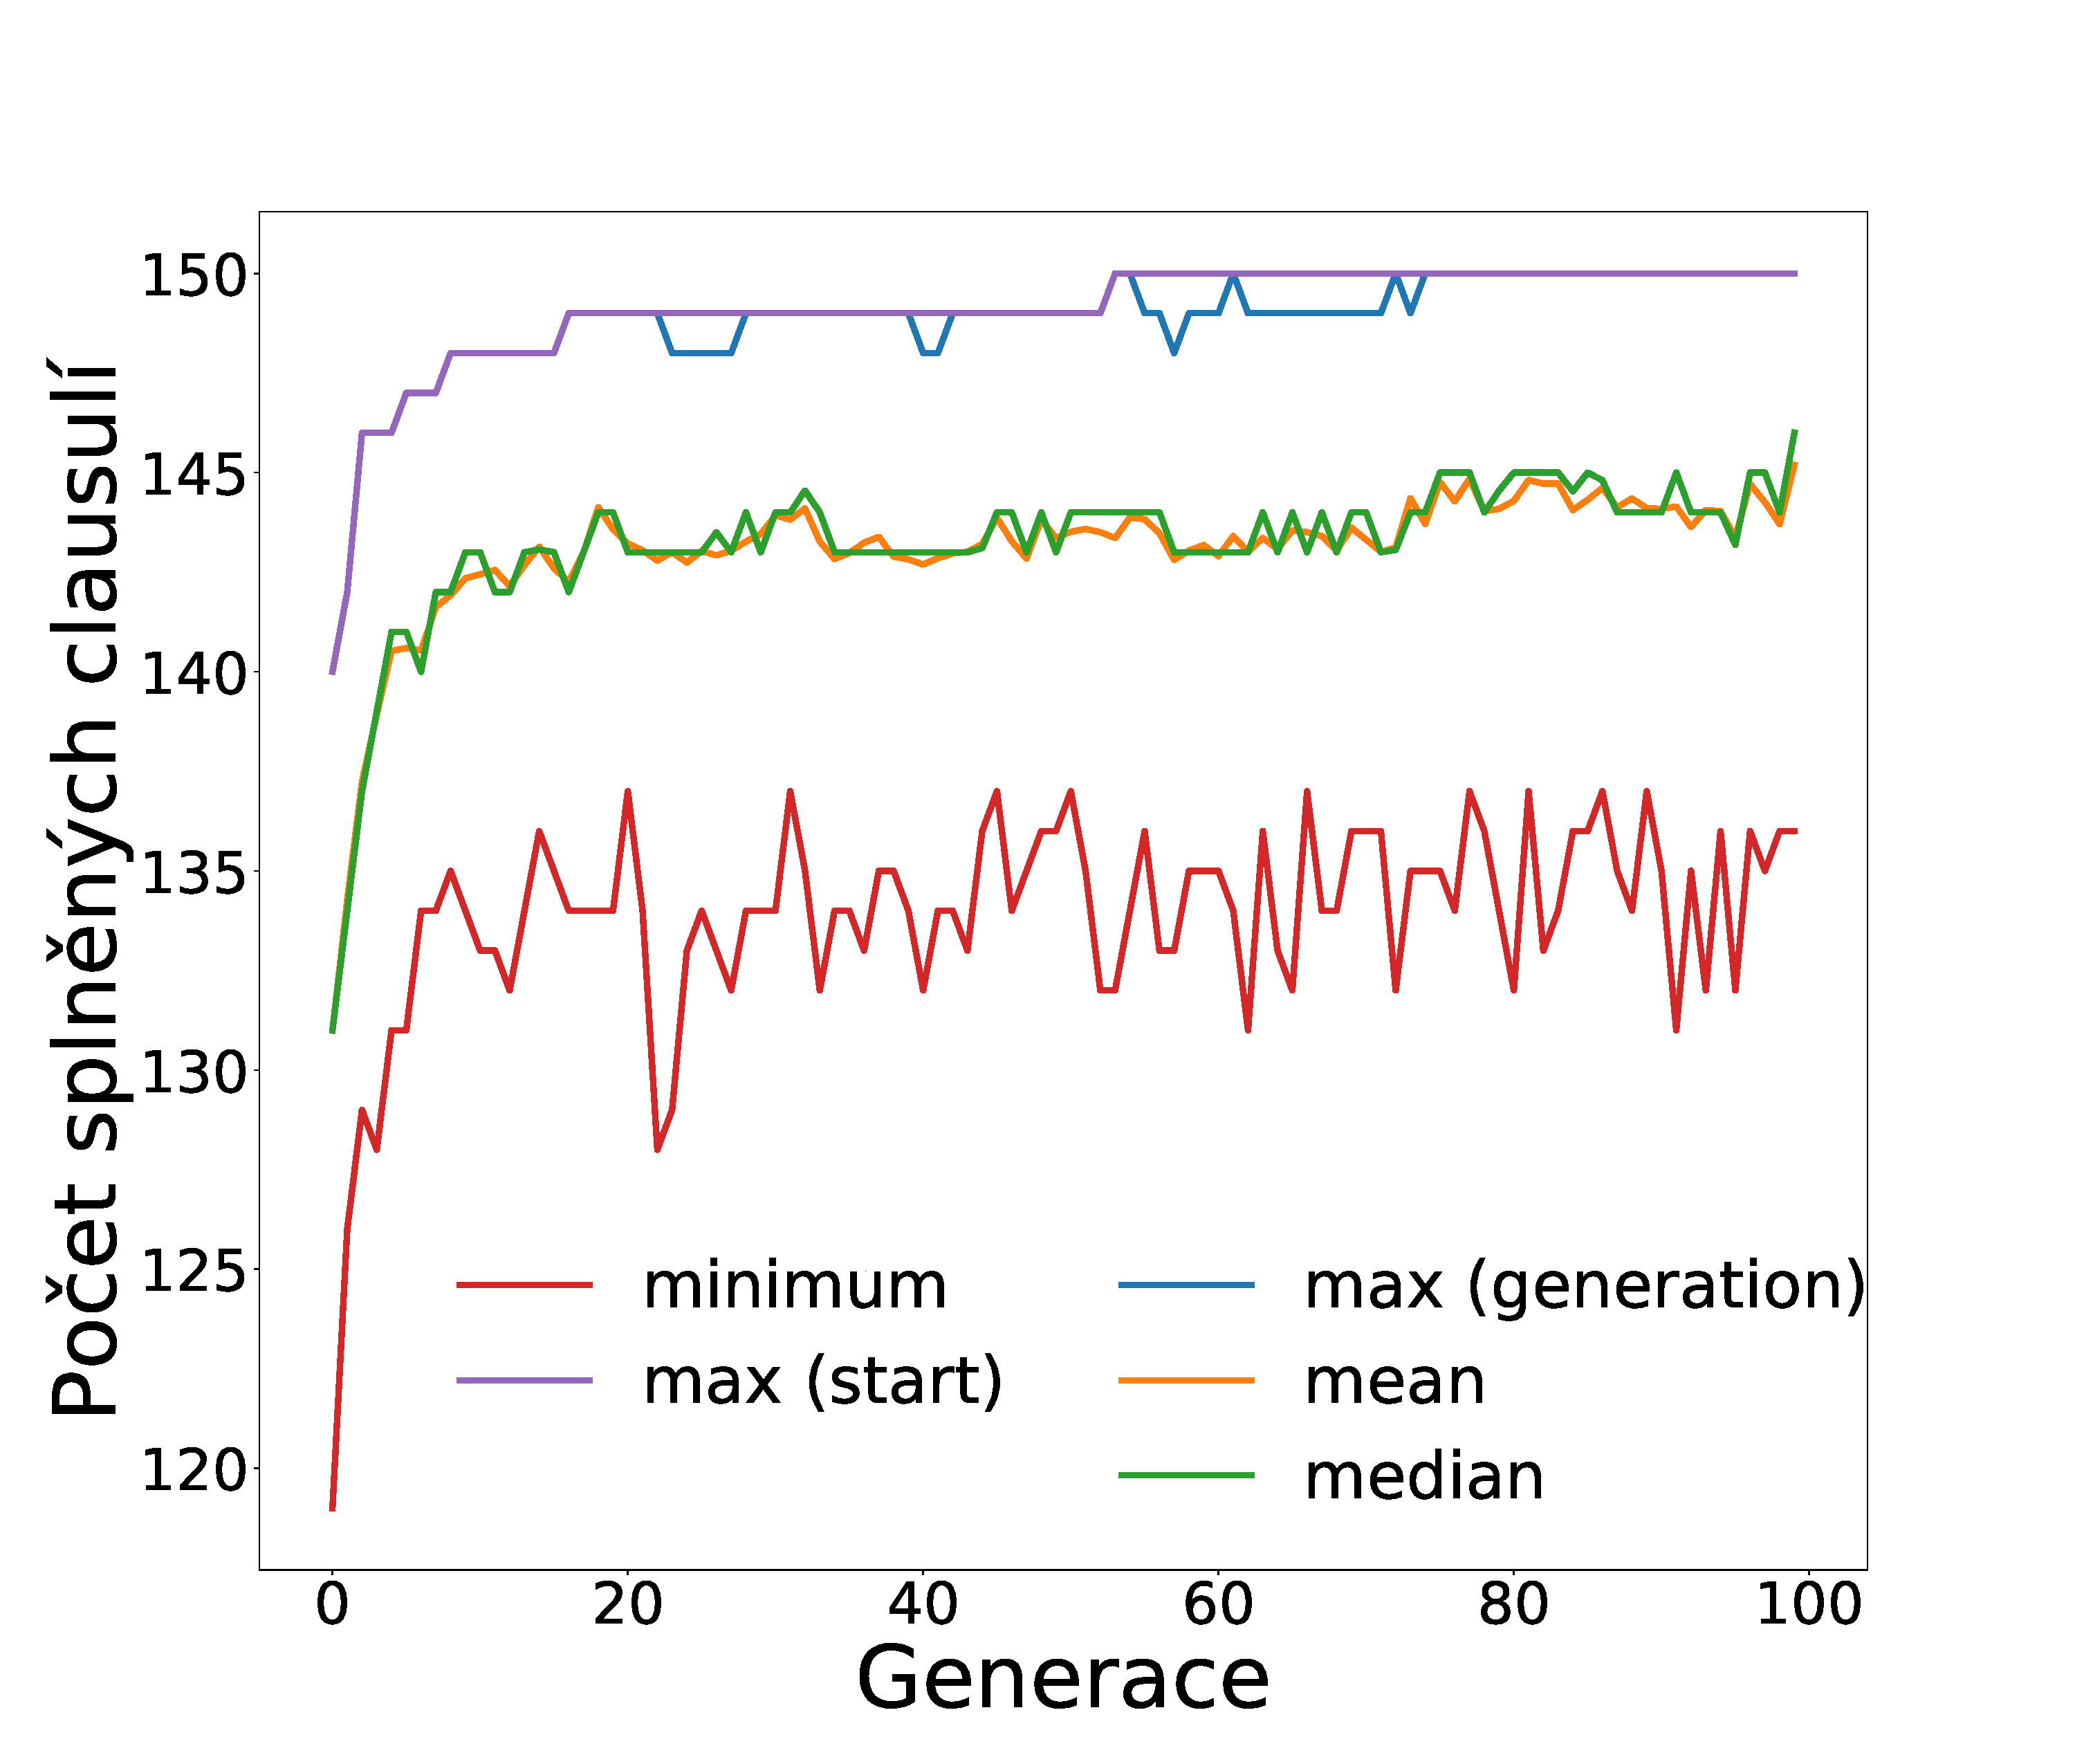
\includegraphics[width=\textwidth]{img/1c.pdf} 
    \end{minipage}
    \begin{minipage}[c]{0.42\textwidth}
        \centering 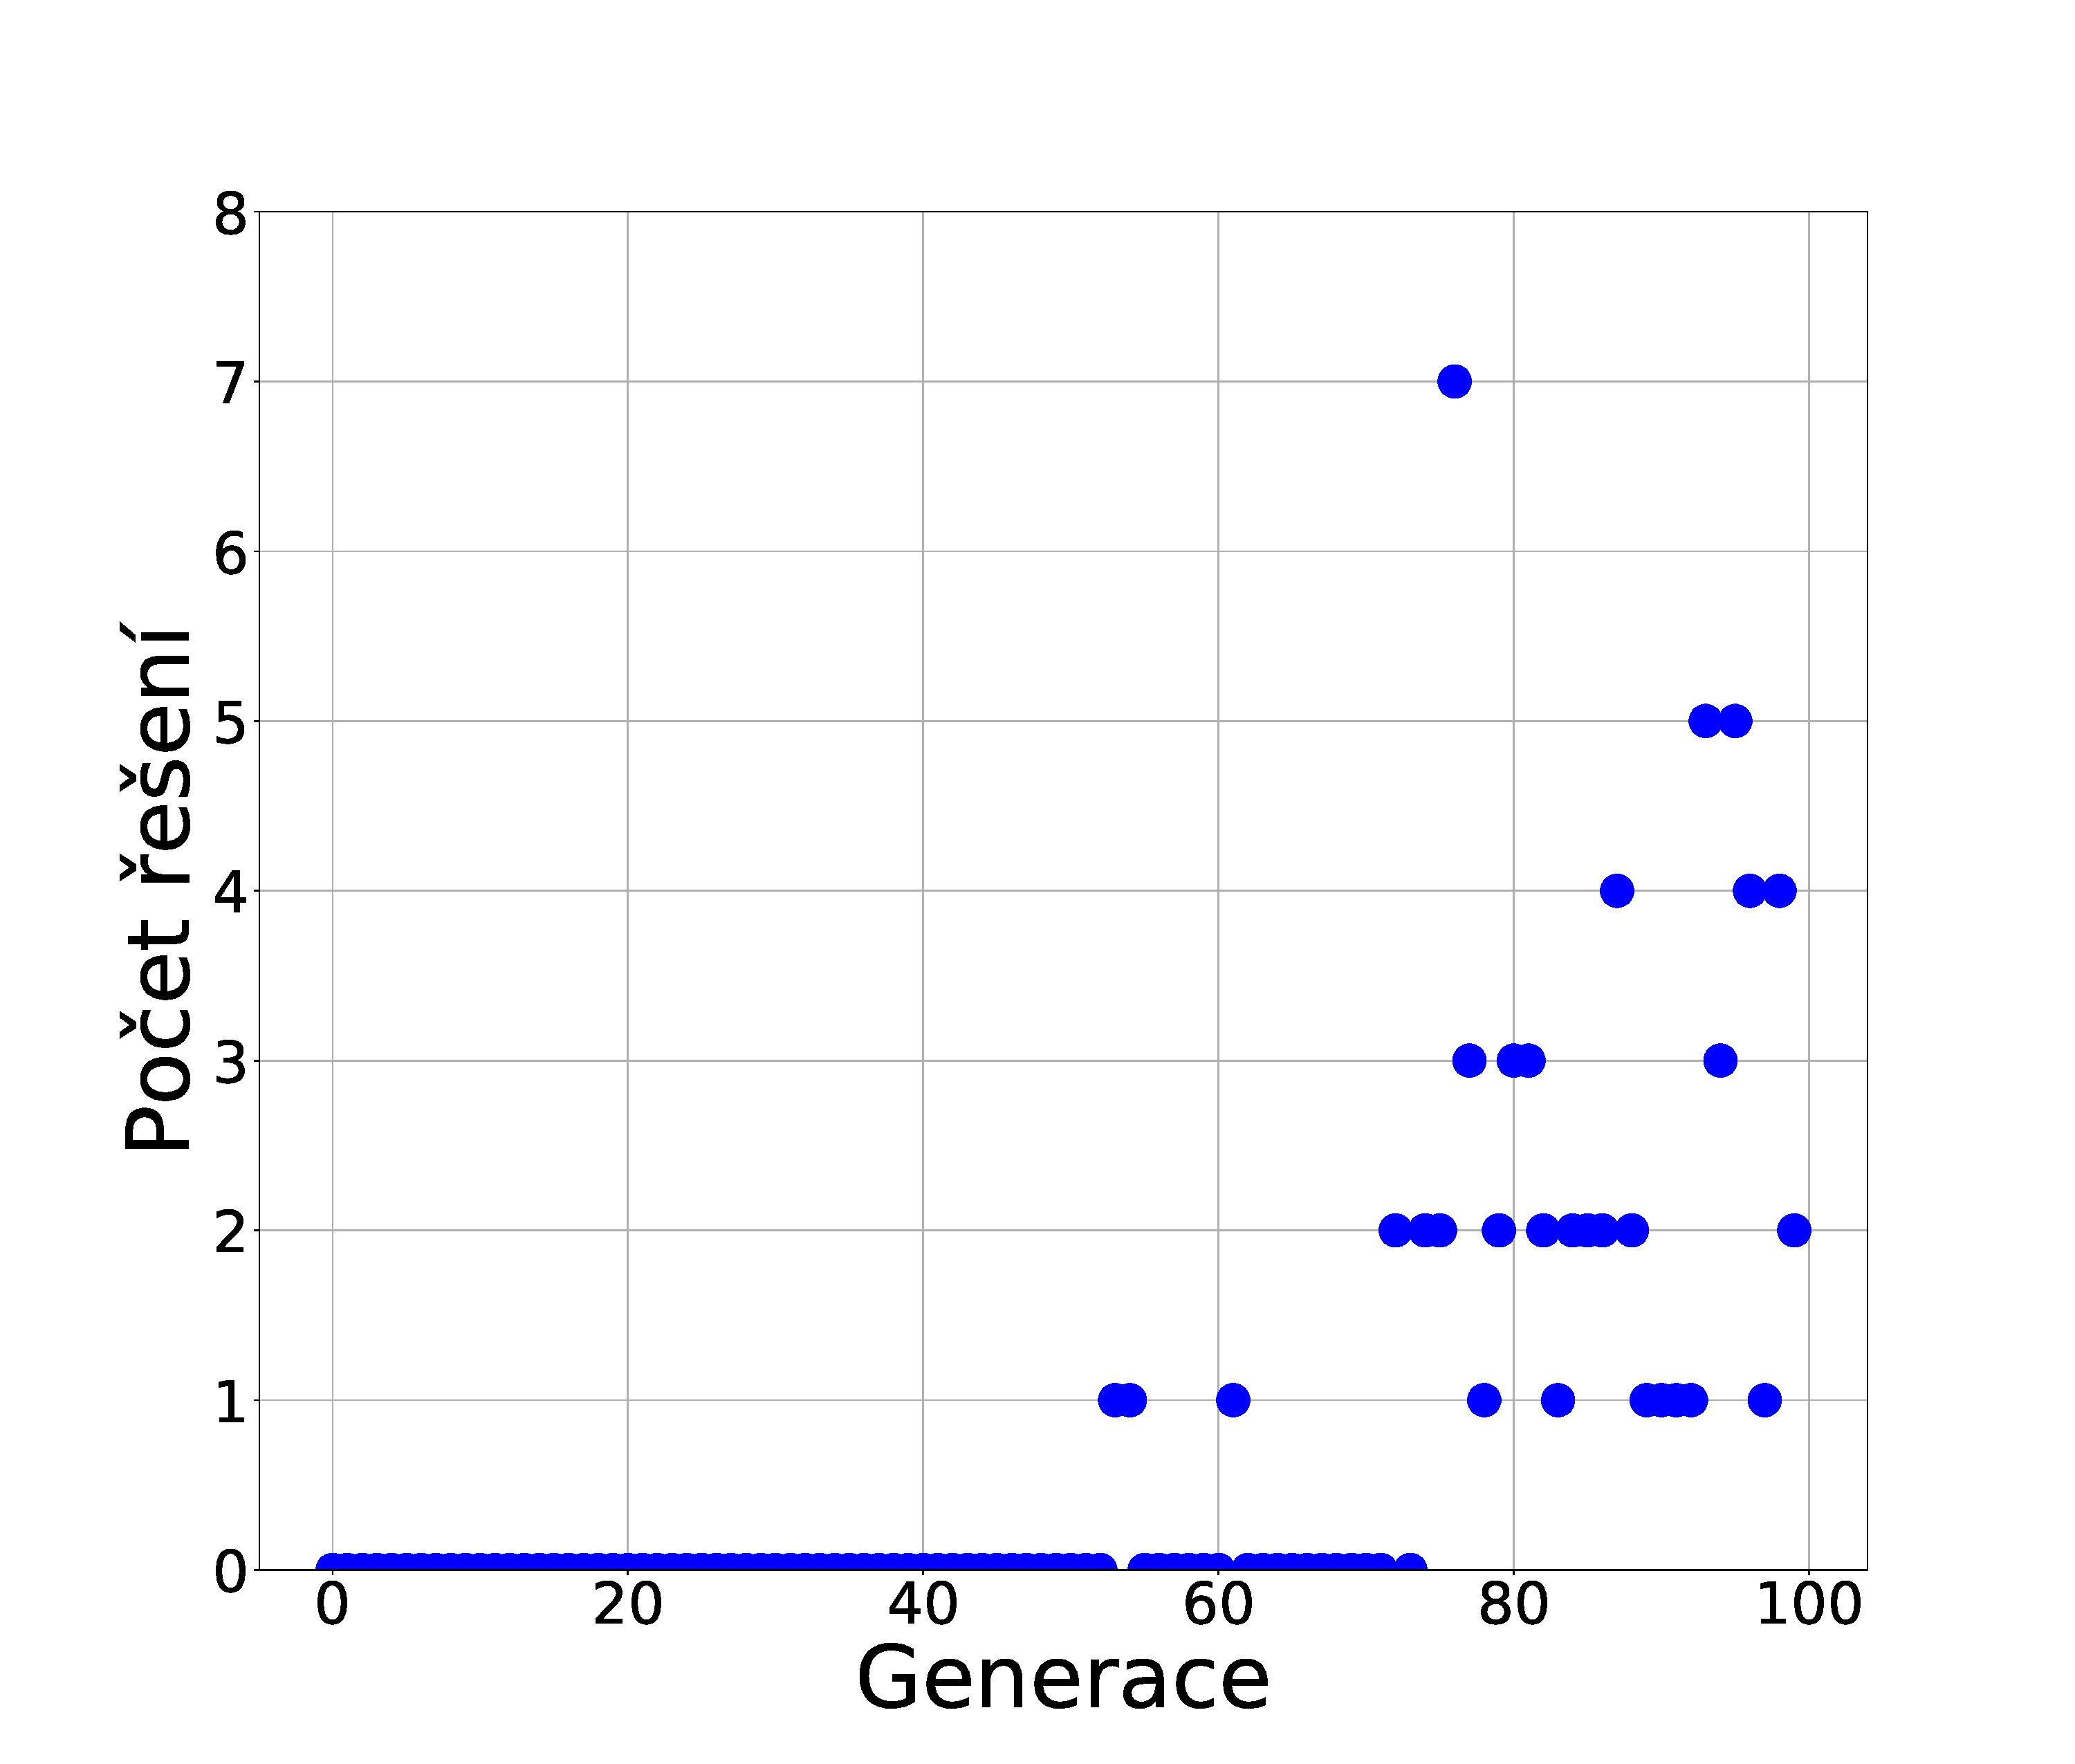
\includegraphics[width=\textwidth]{img/1s.pdf} 
    \end{minipage}
    \\
   \caption{Na levém grafu je závislost relativní chyby na koeficientu ochlazování. Na pravém grafu je závislost výpočetního času na koeficientu ochlazování}\label{fig:GZNK}
\end{figure} 



\begin{figure}
	\centering
    \begin{minipage}[c]{0.48\textwidth}
        \centering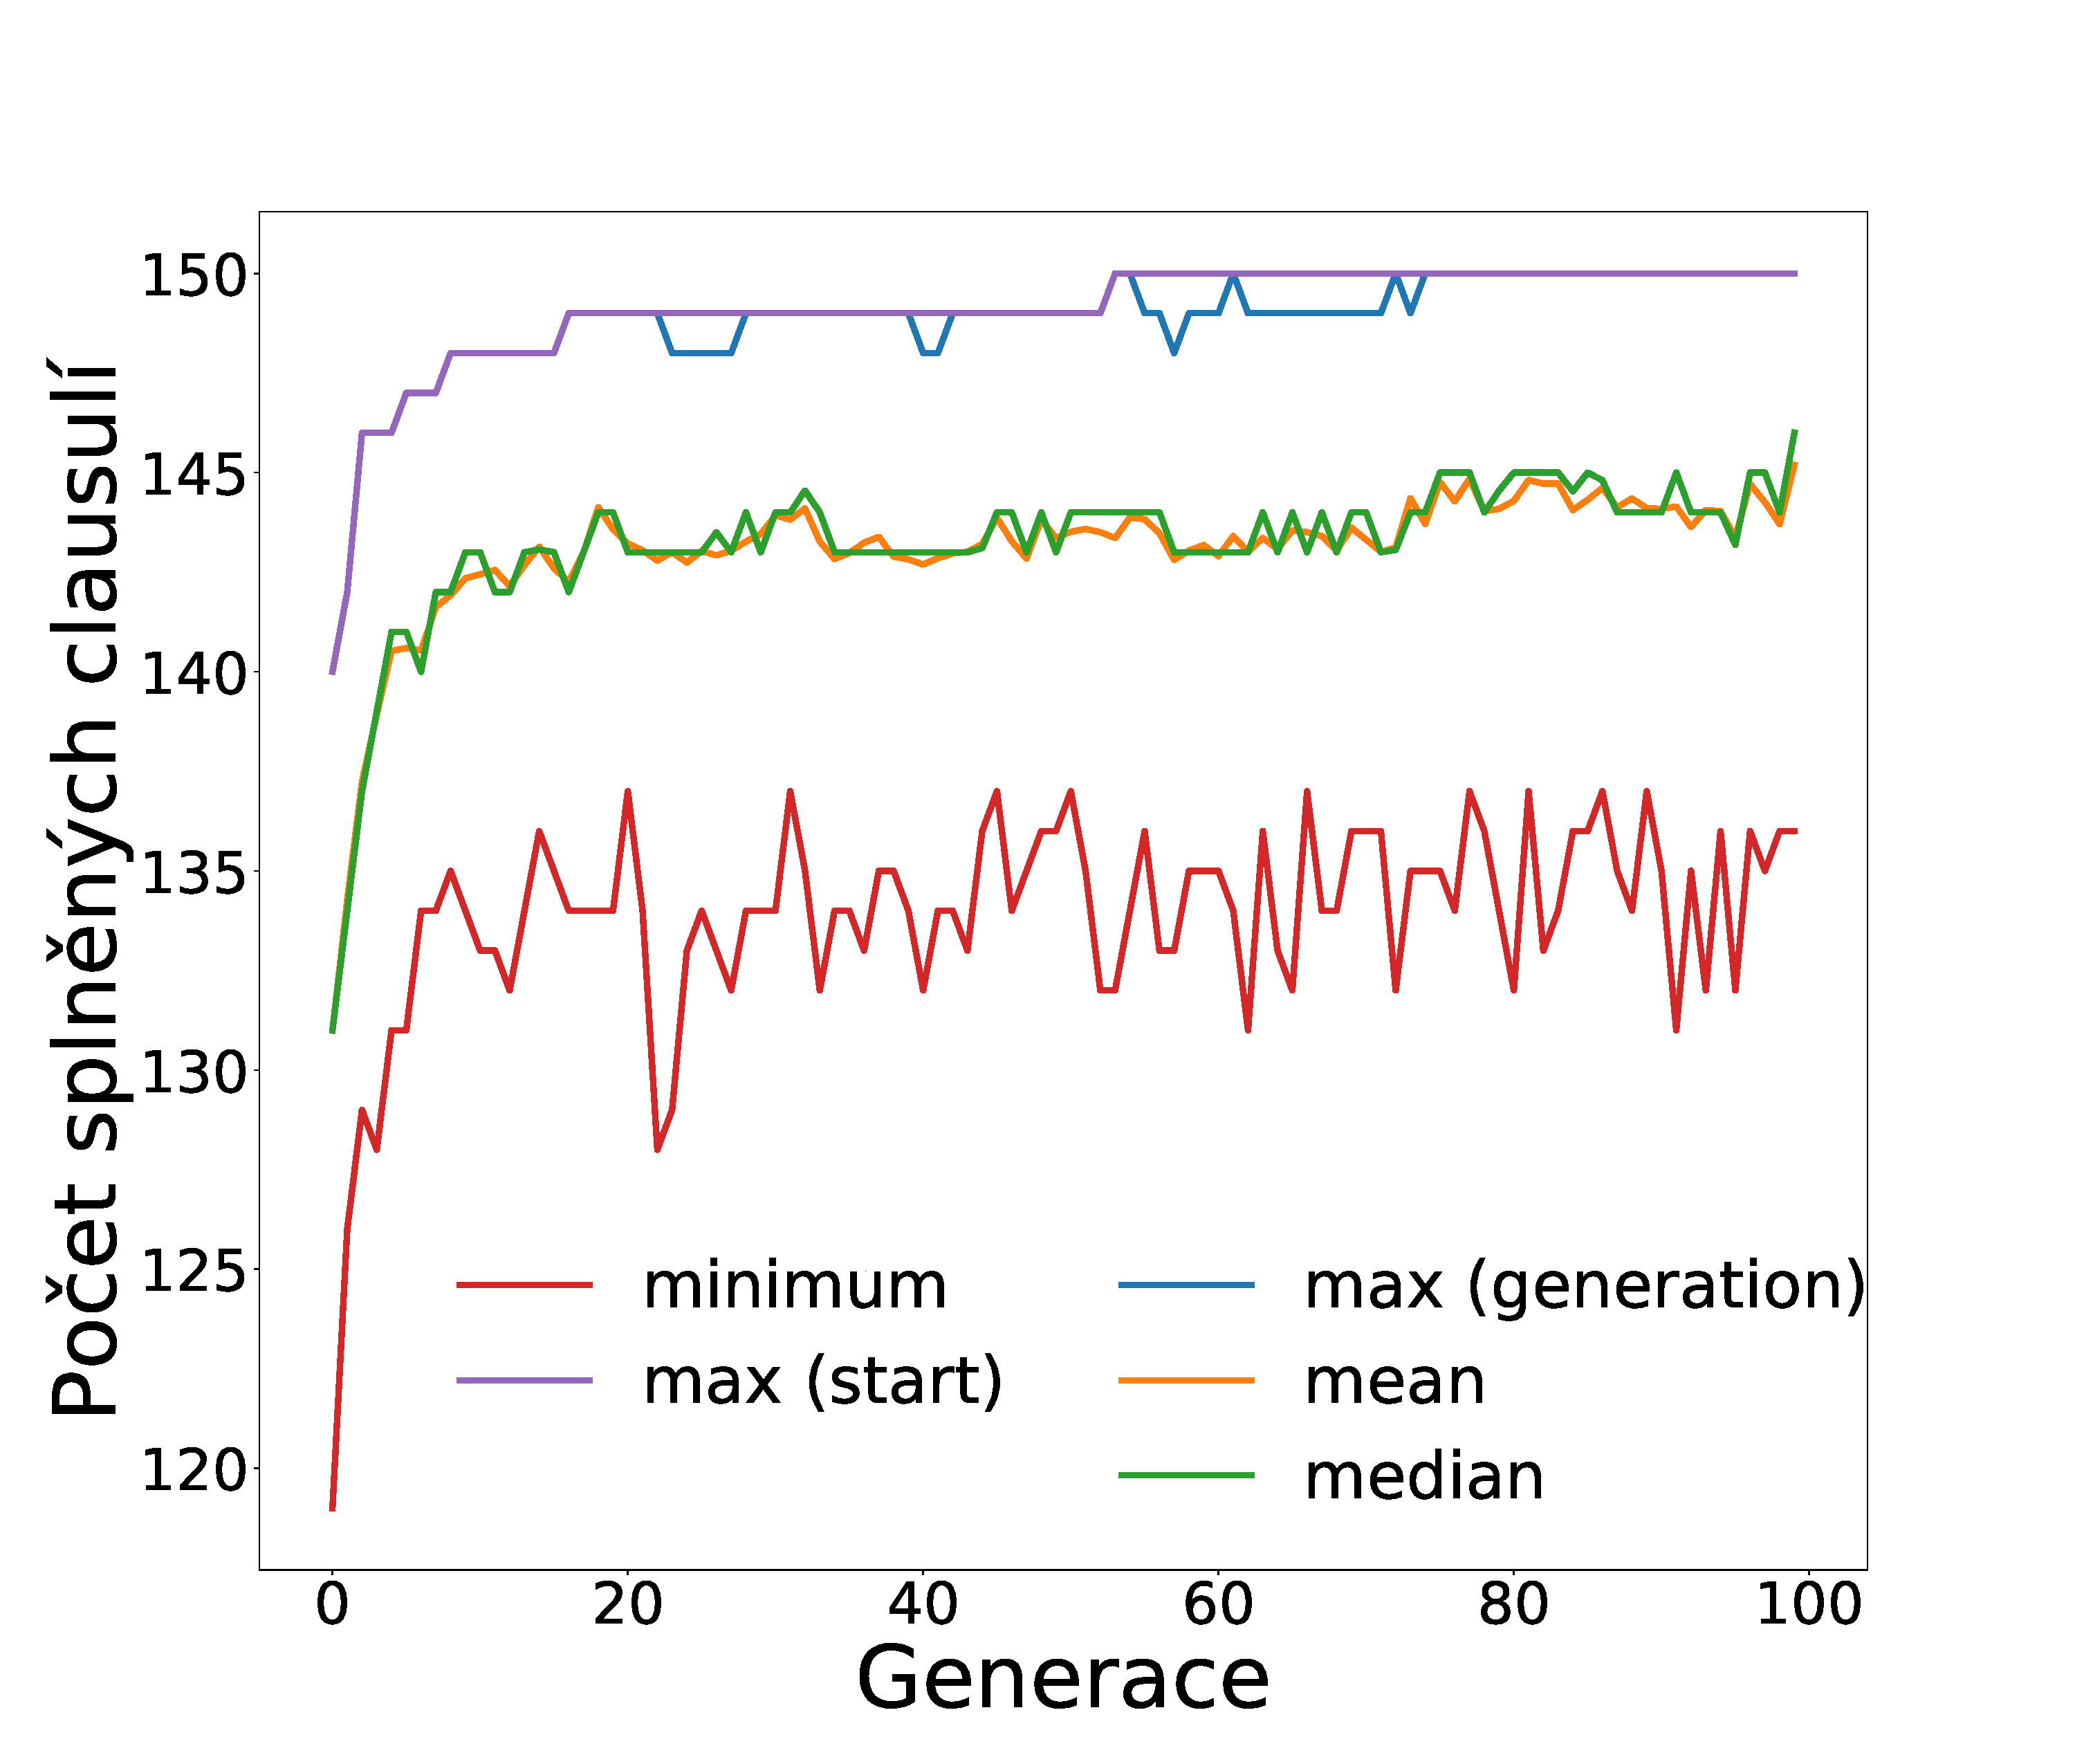
\includegraphics[width=\textwidth]{img/1c.pdf} 
    \end{minipage}
    \begin{minipage}[c]{0.48\textwidth}
        \centering 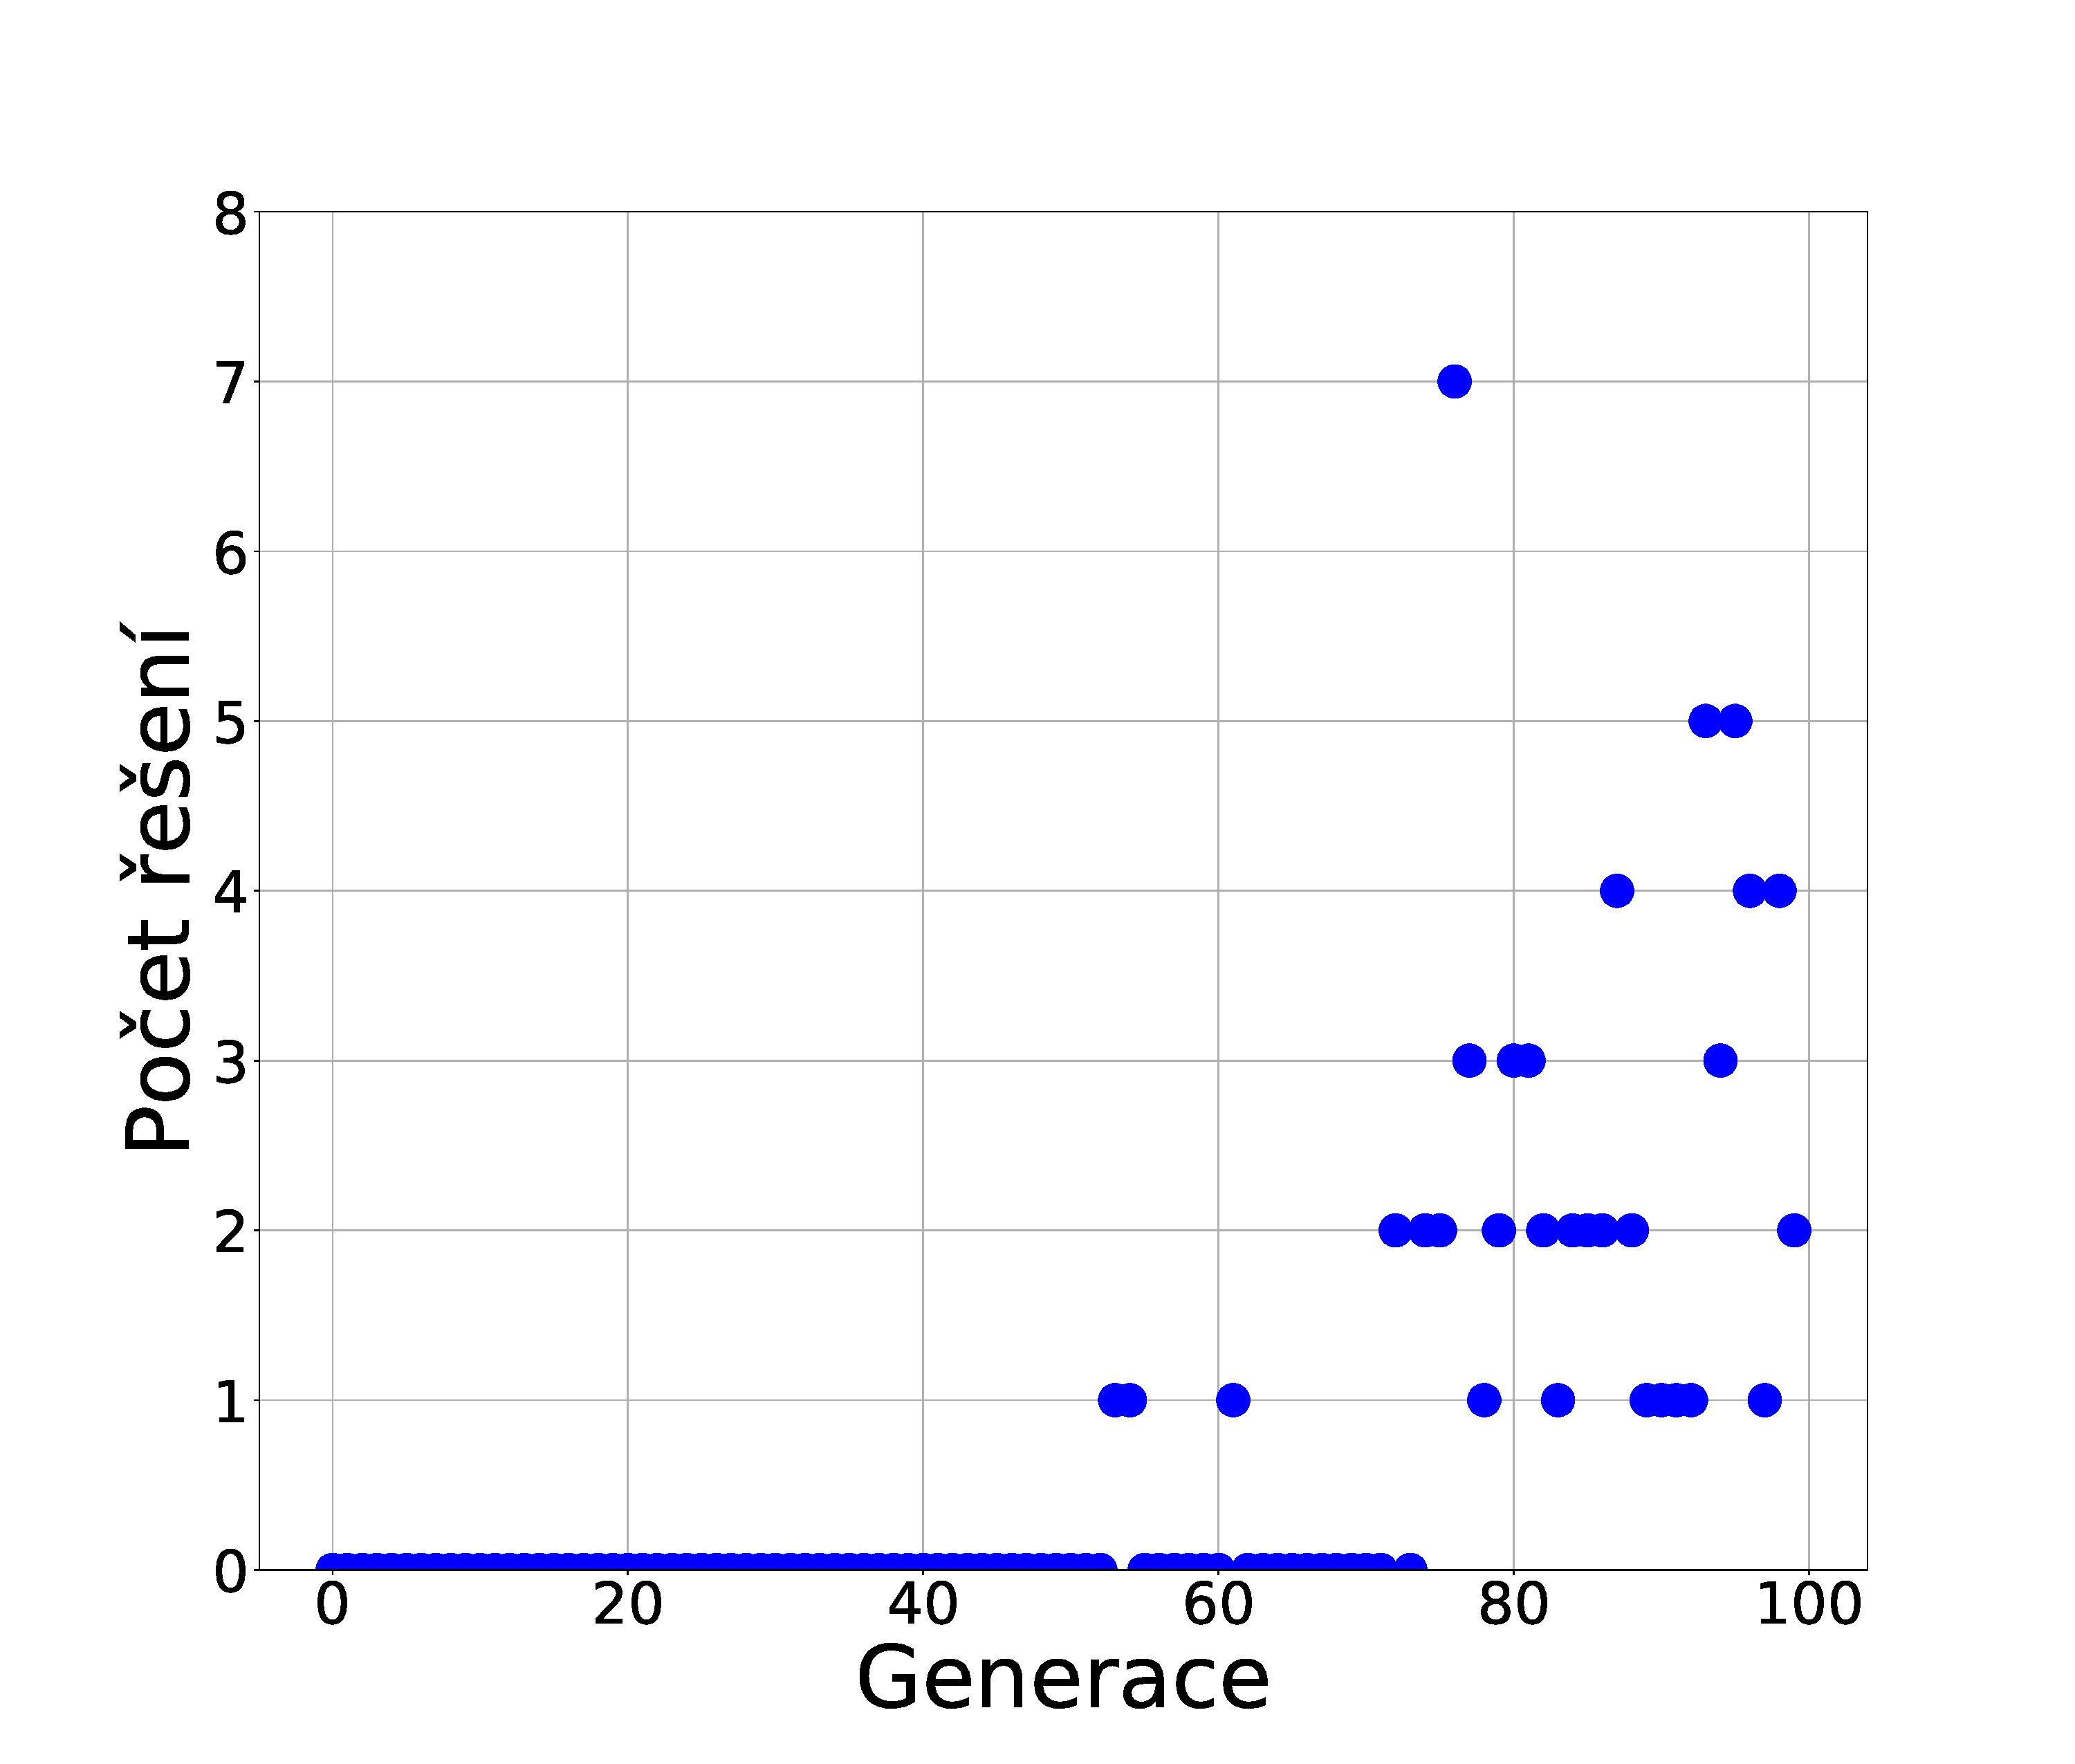
\includegraphics[width=\textwidth]{img/1s.pdf} 
    \end{minipage}
    \\
    \begin{minipage}[c]{0.48\textwidth}
        \centering 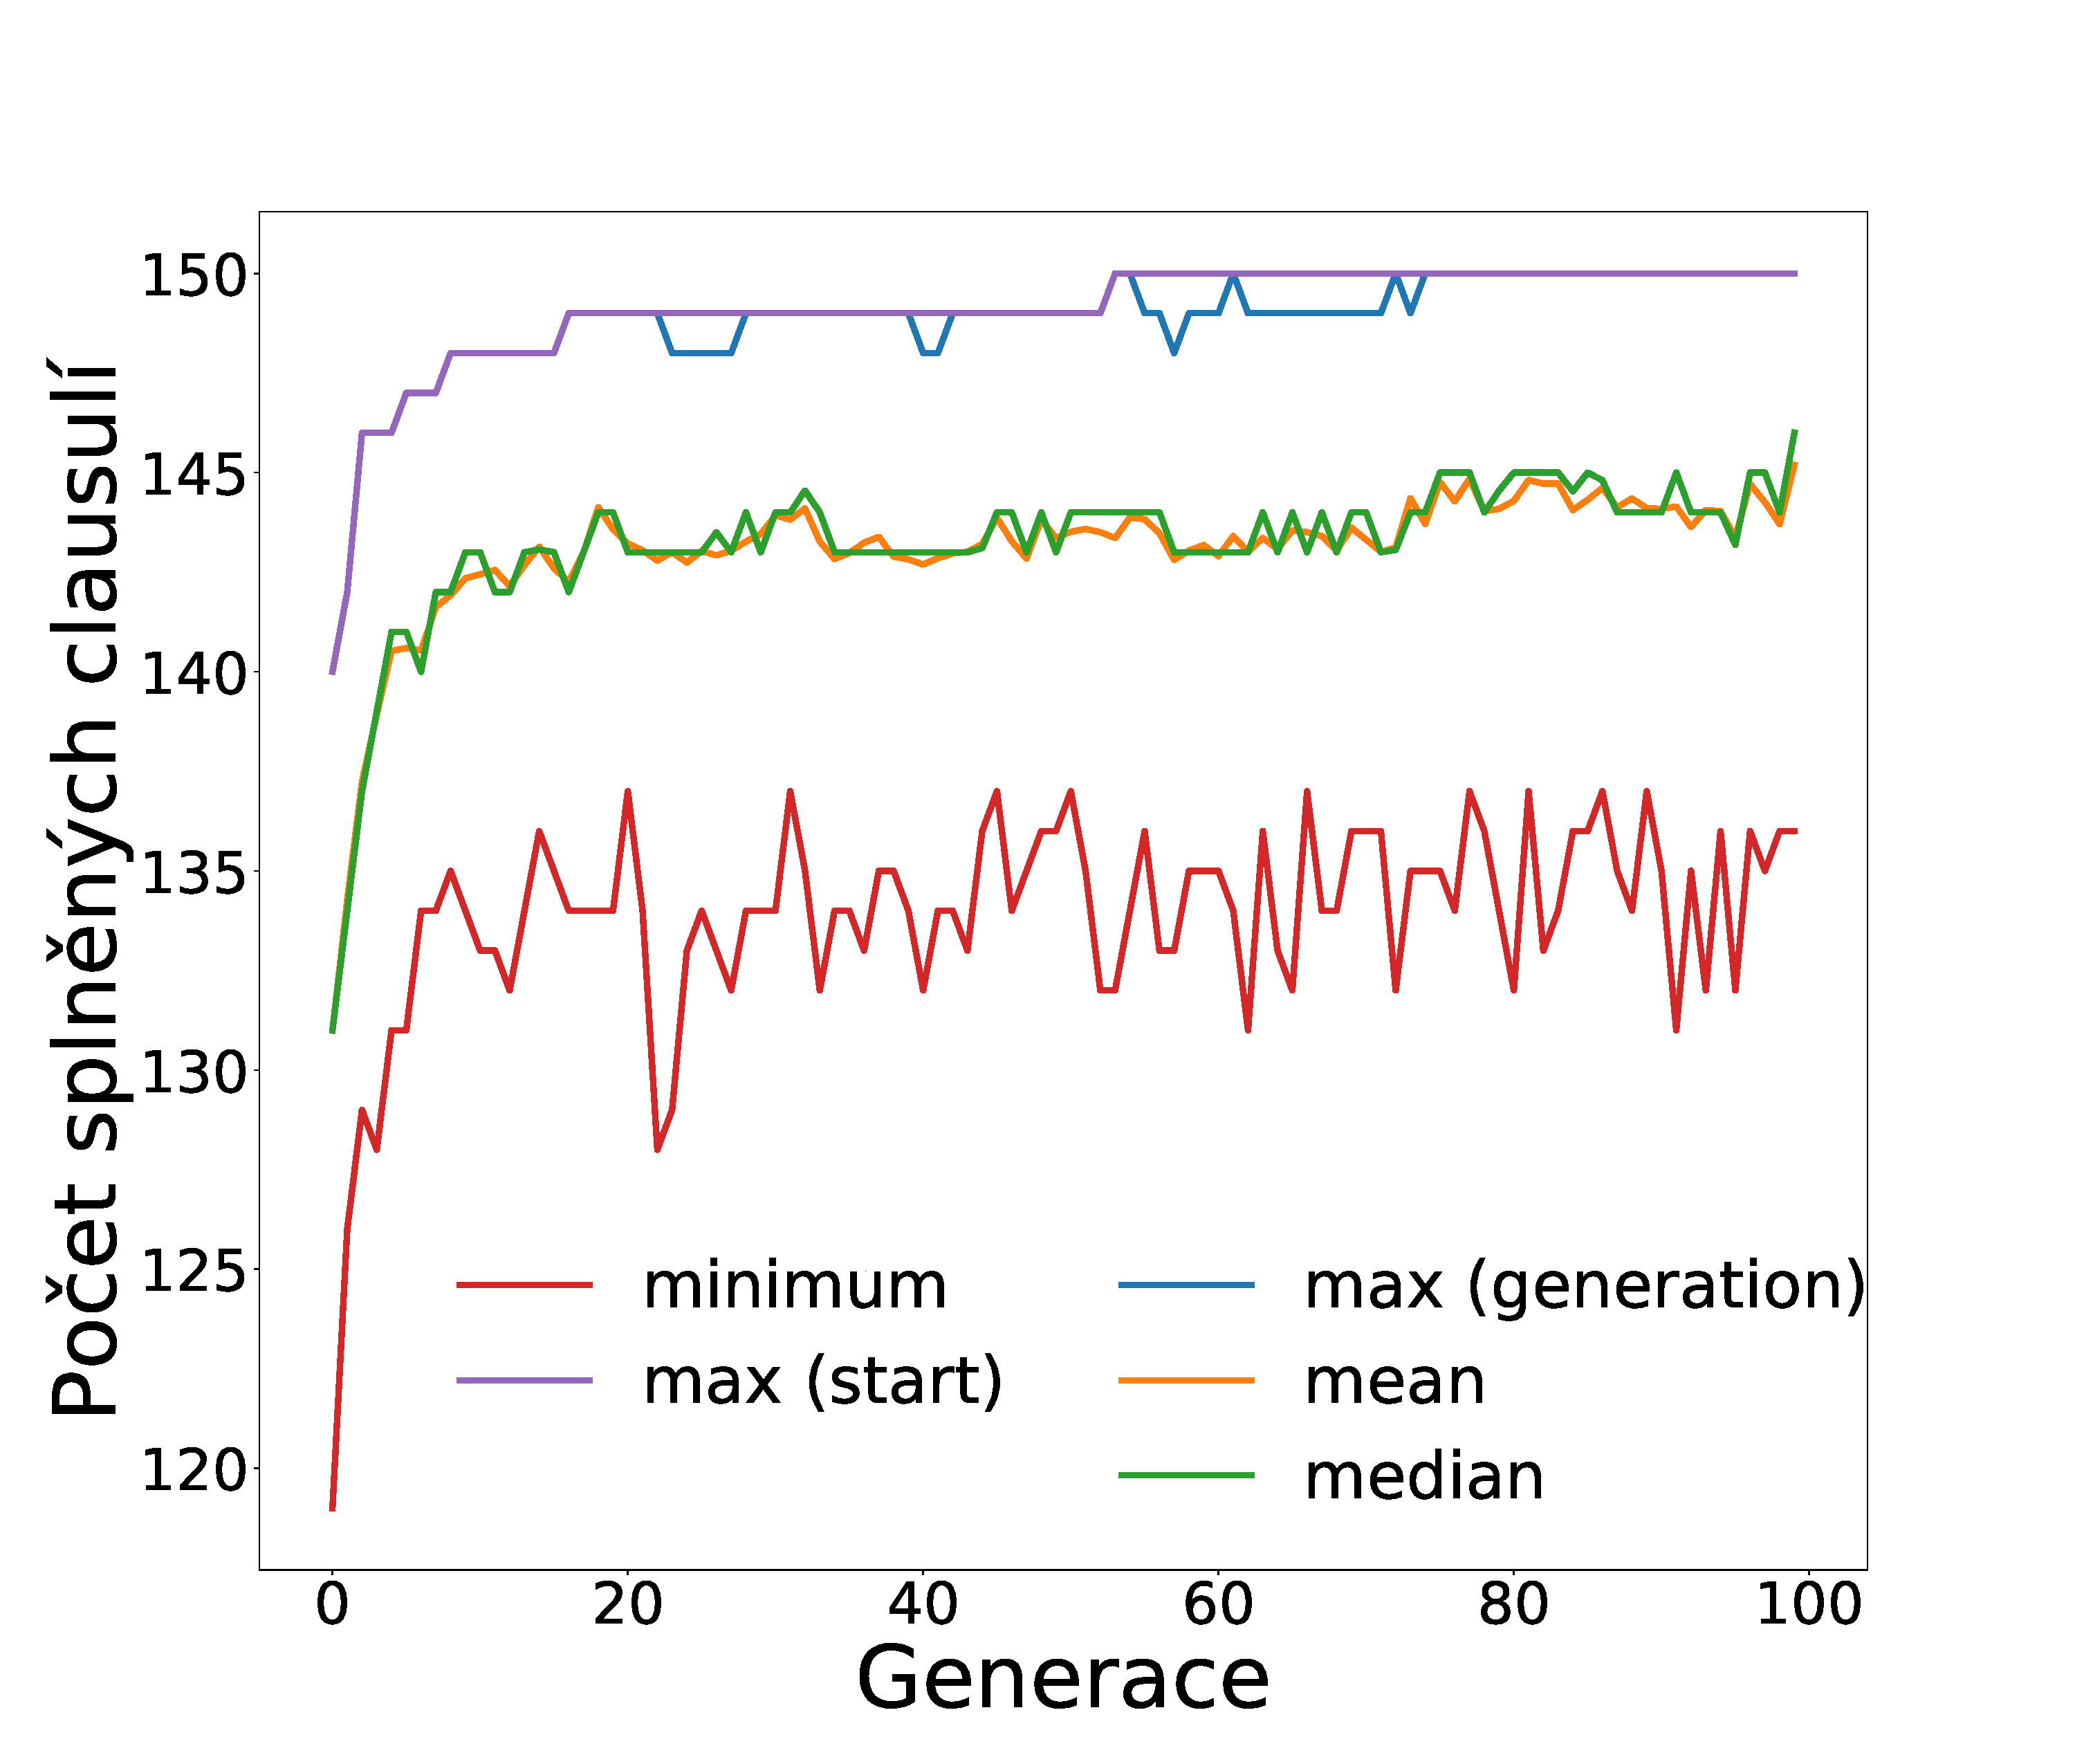
\includegraphics[width=\textwidth]{img/1c.pdf} 
    \end{minipage}
    \begin{minipage}[c]{0.48\textwidth}
        \centering 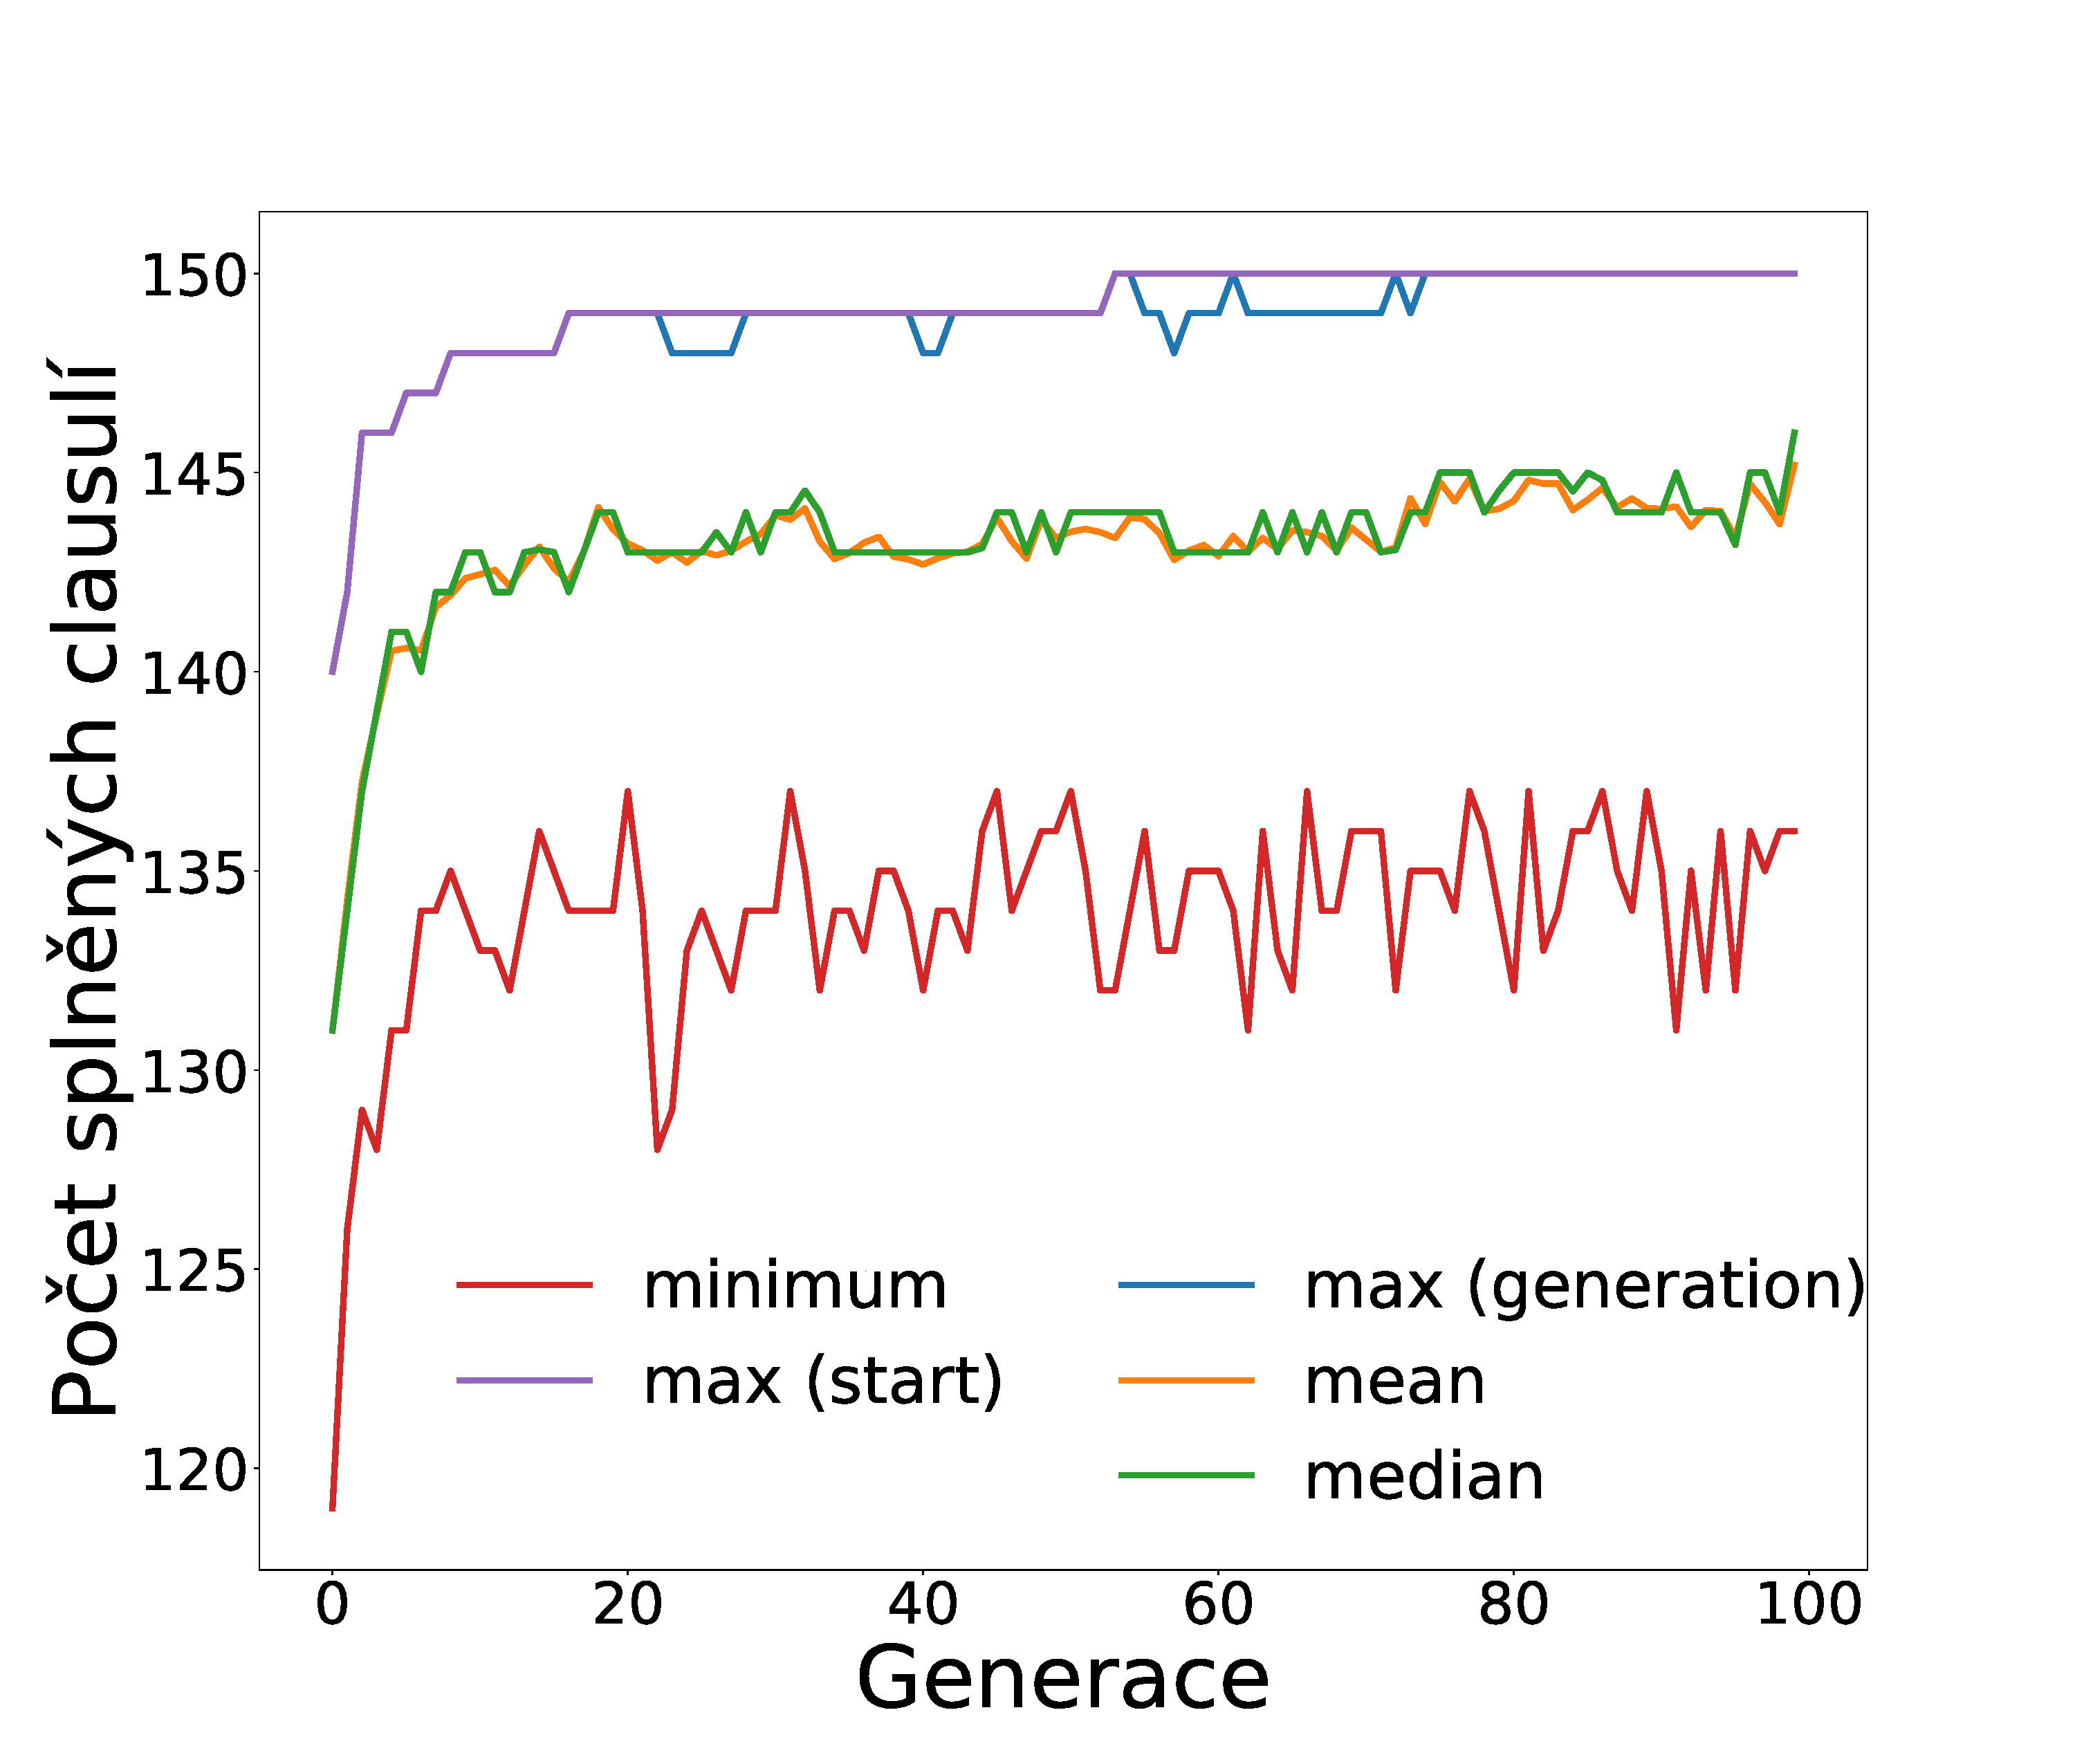
\includegraphics[width=\textwidth]{img/1c.pdf} 
    \end{minipage}
   \caption{Zde jsou uvedené grafy vývoje řešení pro vybrané hodnoty koeficientu ochlazovaní. Konkrétně zleva pro hodnoty 0.993, 0.995, 0.997, 0.999}\label{fig:GVPK}
\end{figure} 

 


 \begin{figure}
	\centering
    \begin{minipage}[c]{0.42\textwidth}
        \centering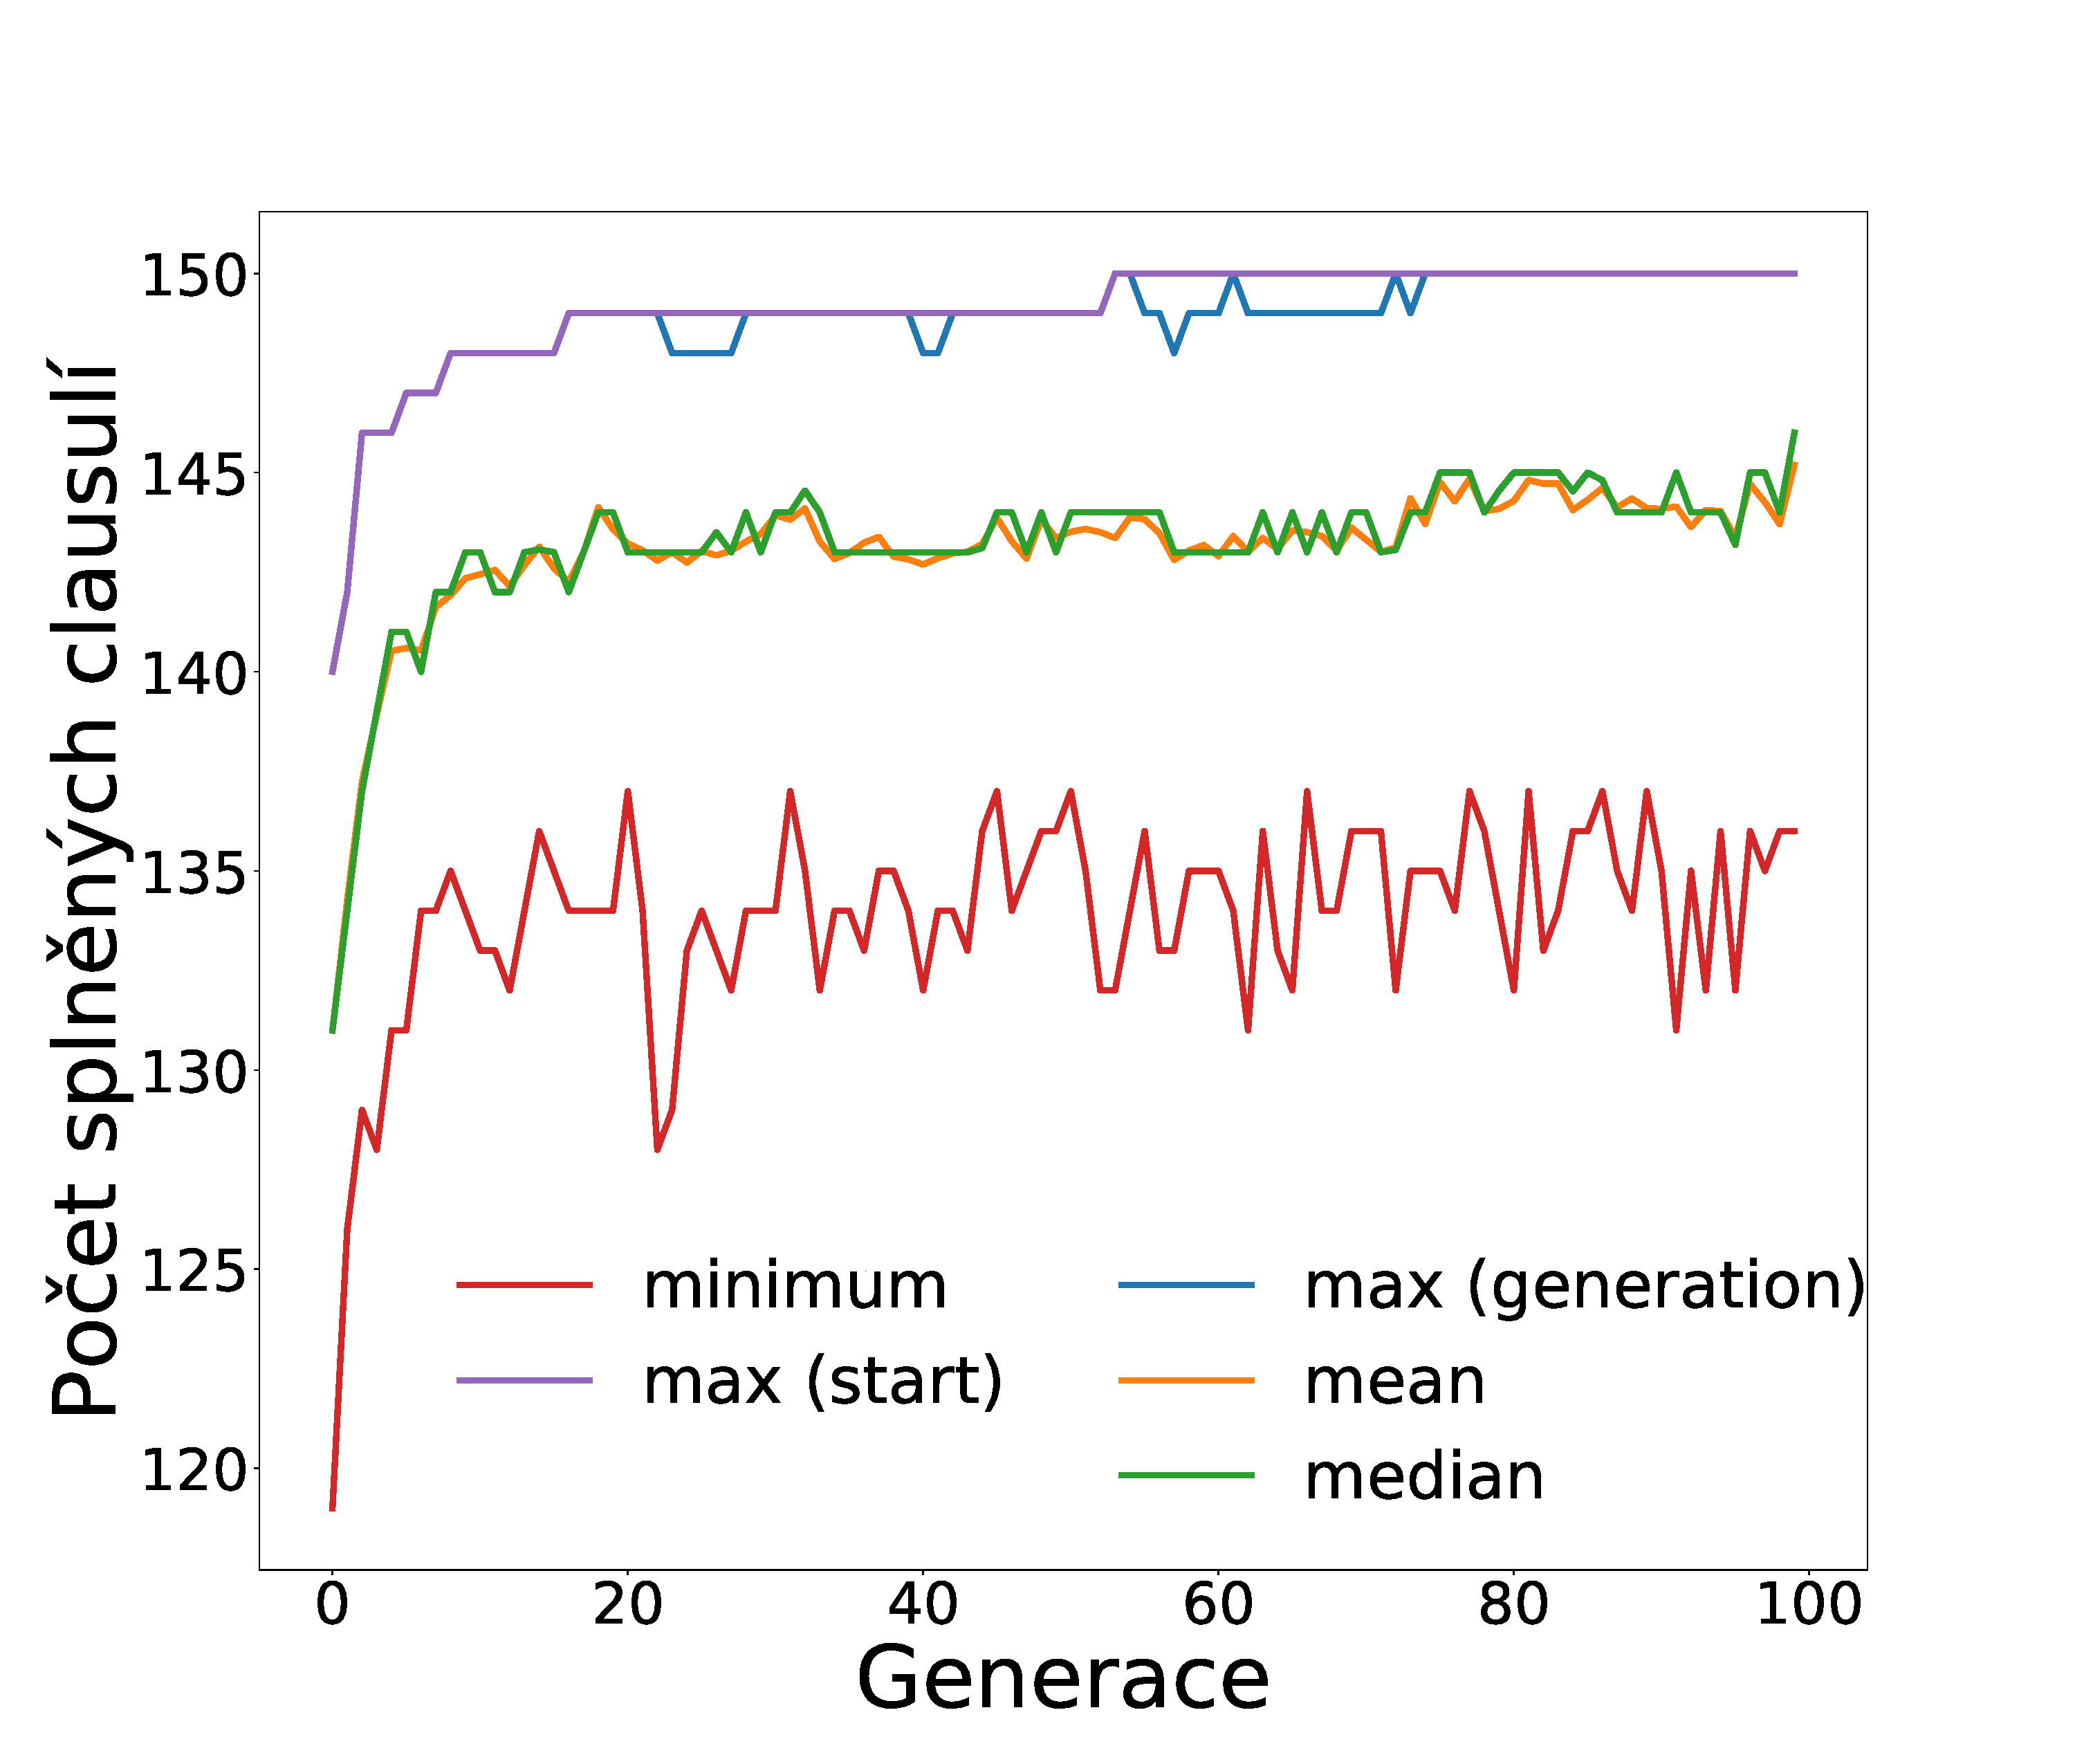
\includegraphics[width=\textwidth]{img/1c.pdf} 
    \end{minipage}
    \begin{minipage}[c]{0.42\textwidth}
        \centering 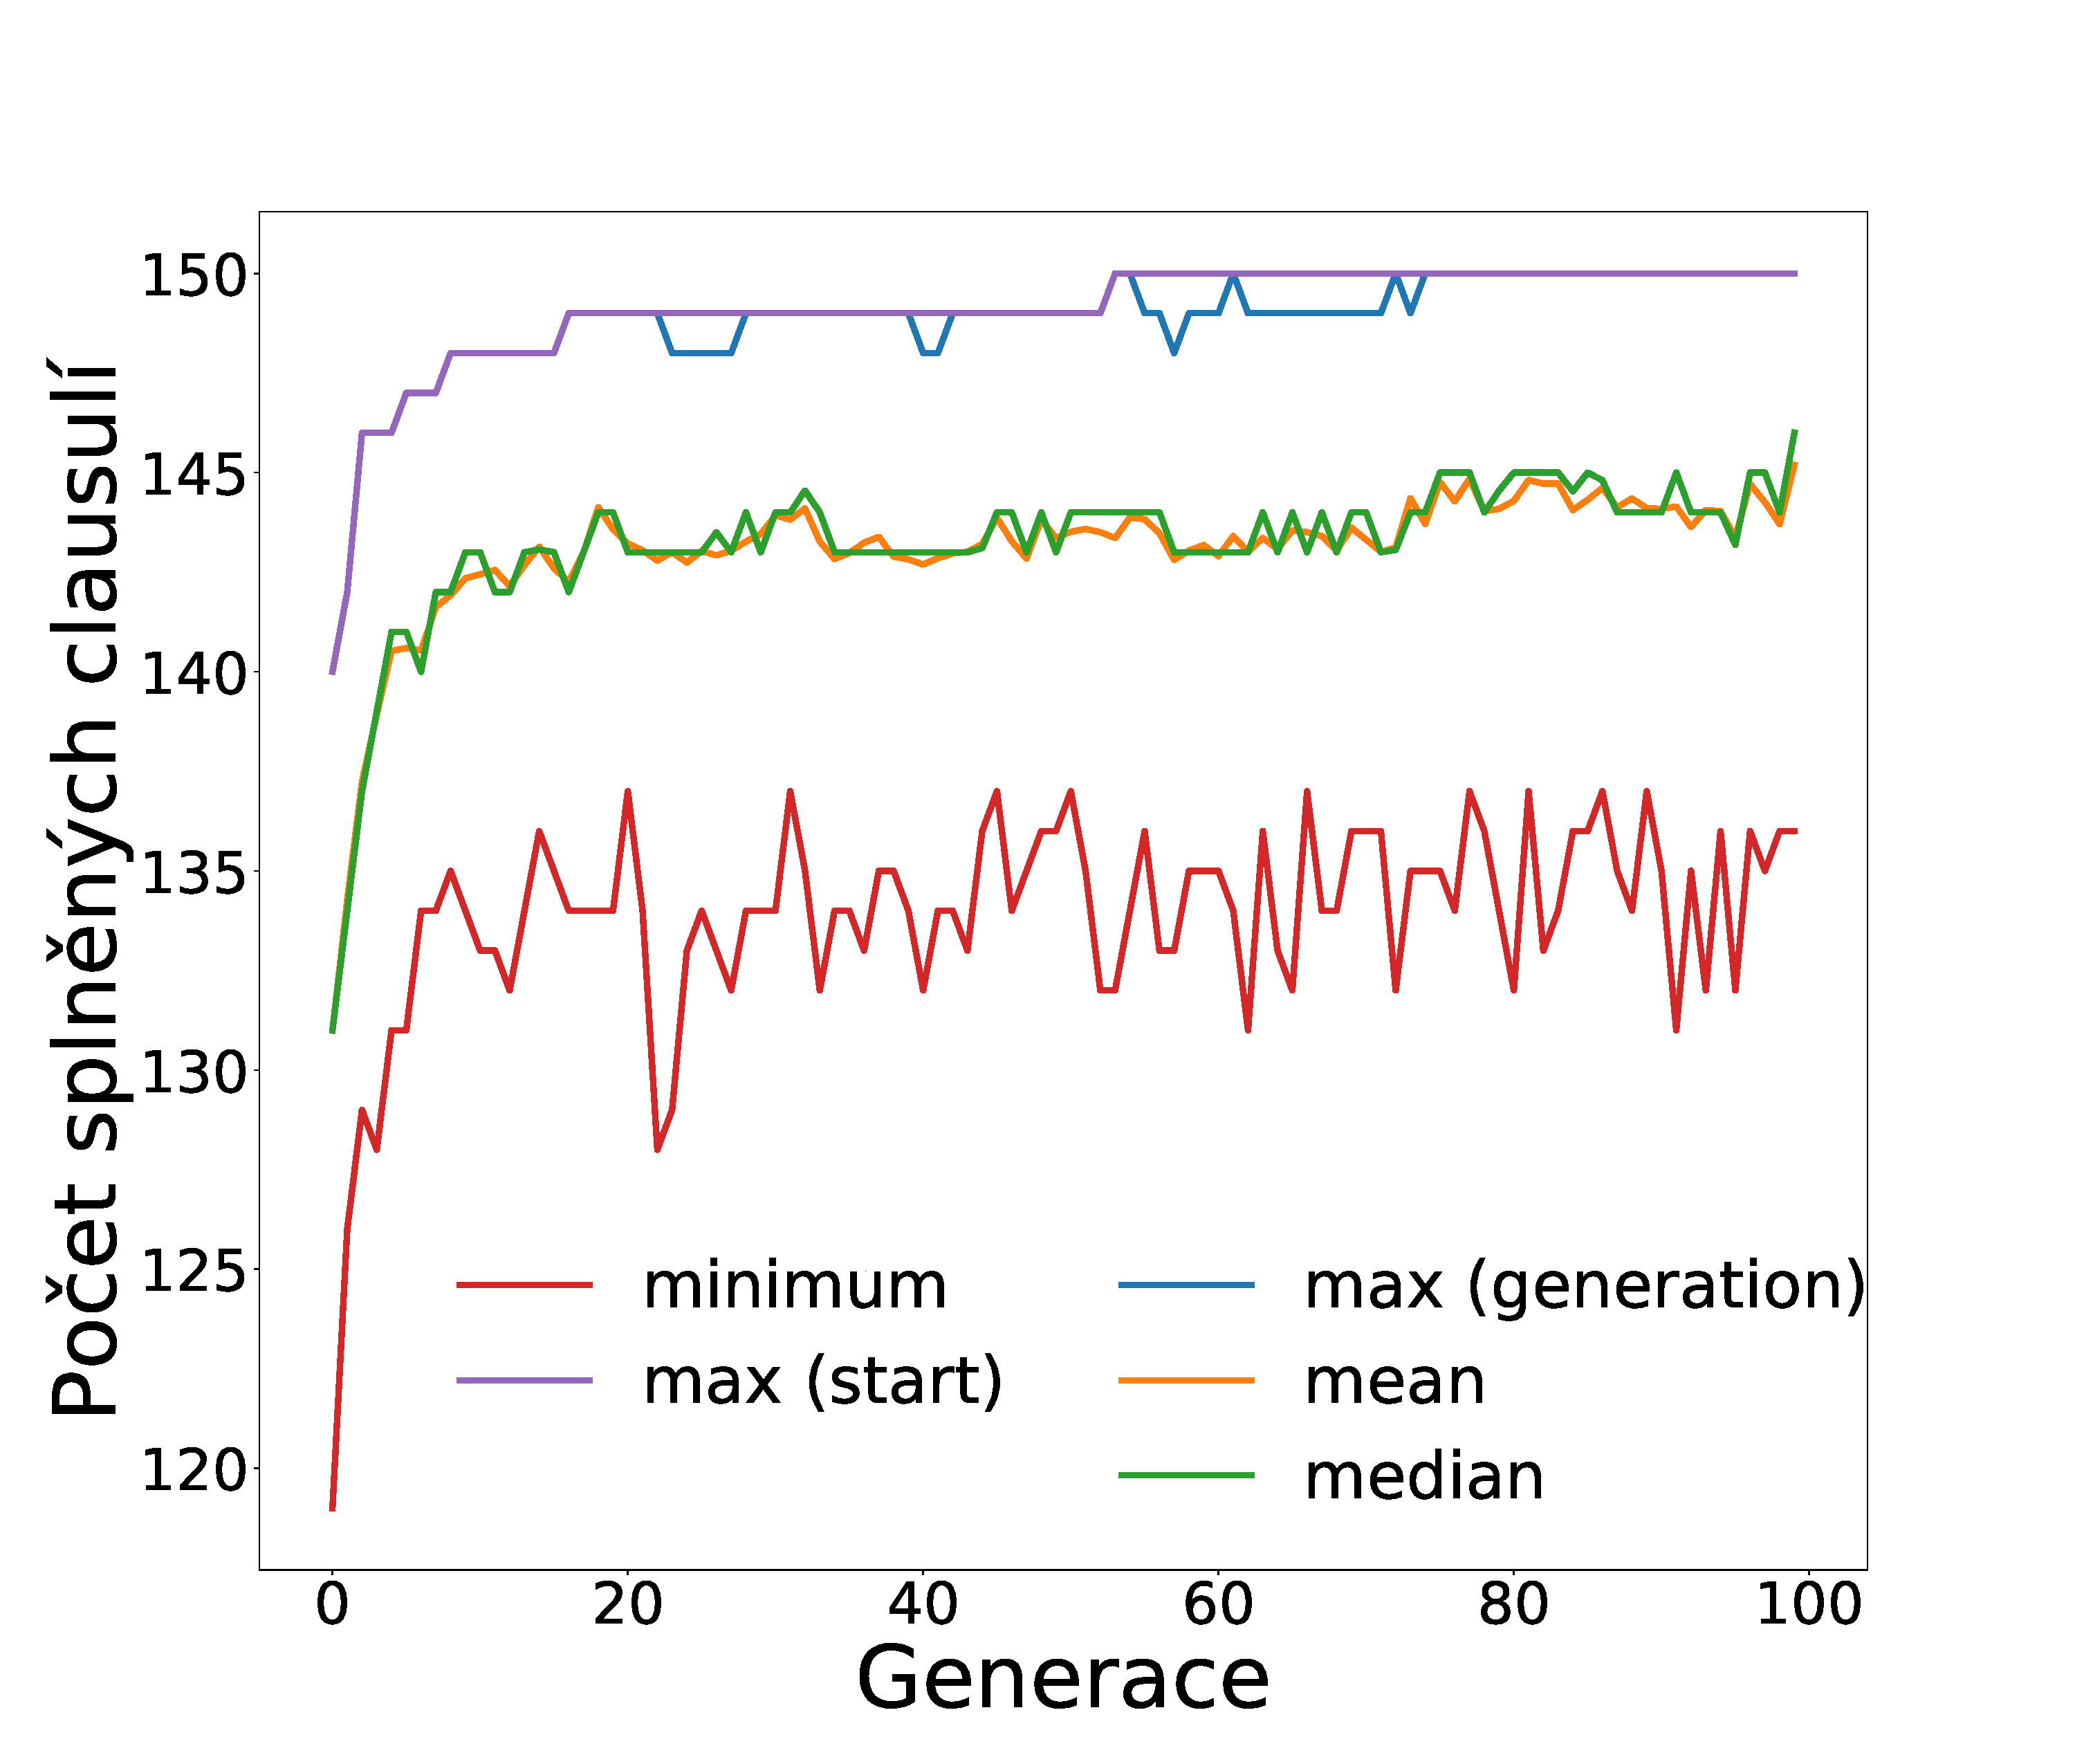
\includegraphics[width=\textwidth]{img/1c.pdf} 
    \end{minipage}
    \\
   \caption{Na levém grafu je závislost relativní chyby na počtu iterací na jedné teplotě. Na pravém grafu je závislost výpočetního času na počtu iterací na jedné teplotě}\label{fig:GZNC}
\end{figure} 

\begin{figure}
	\centering
    \begin{minipage}[c]{0.32\textwidth}
        \centering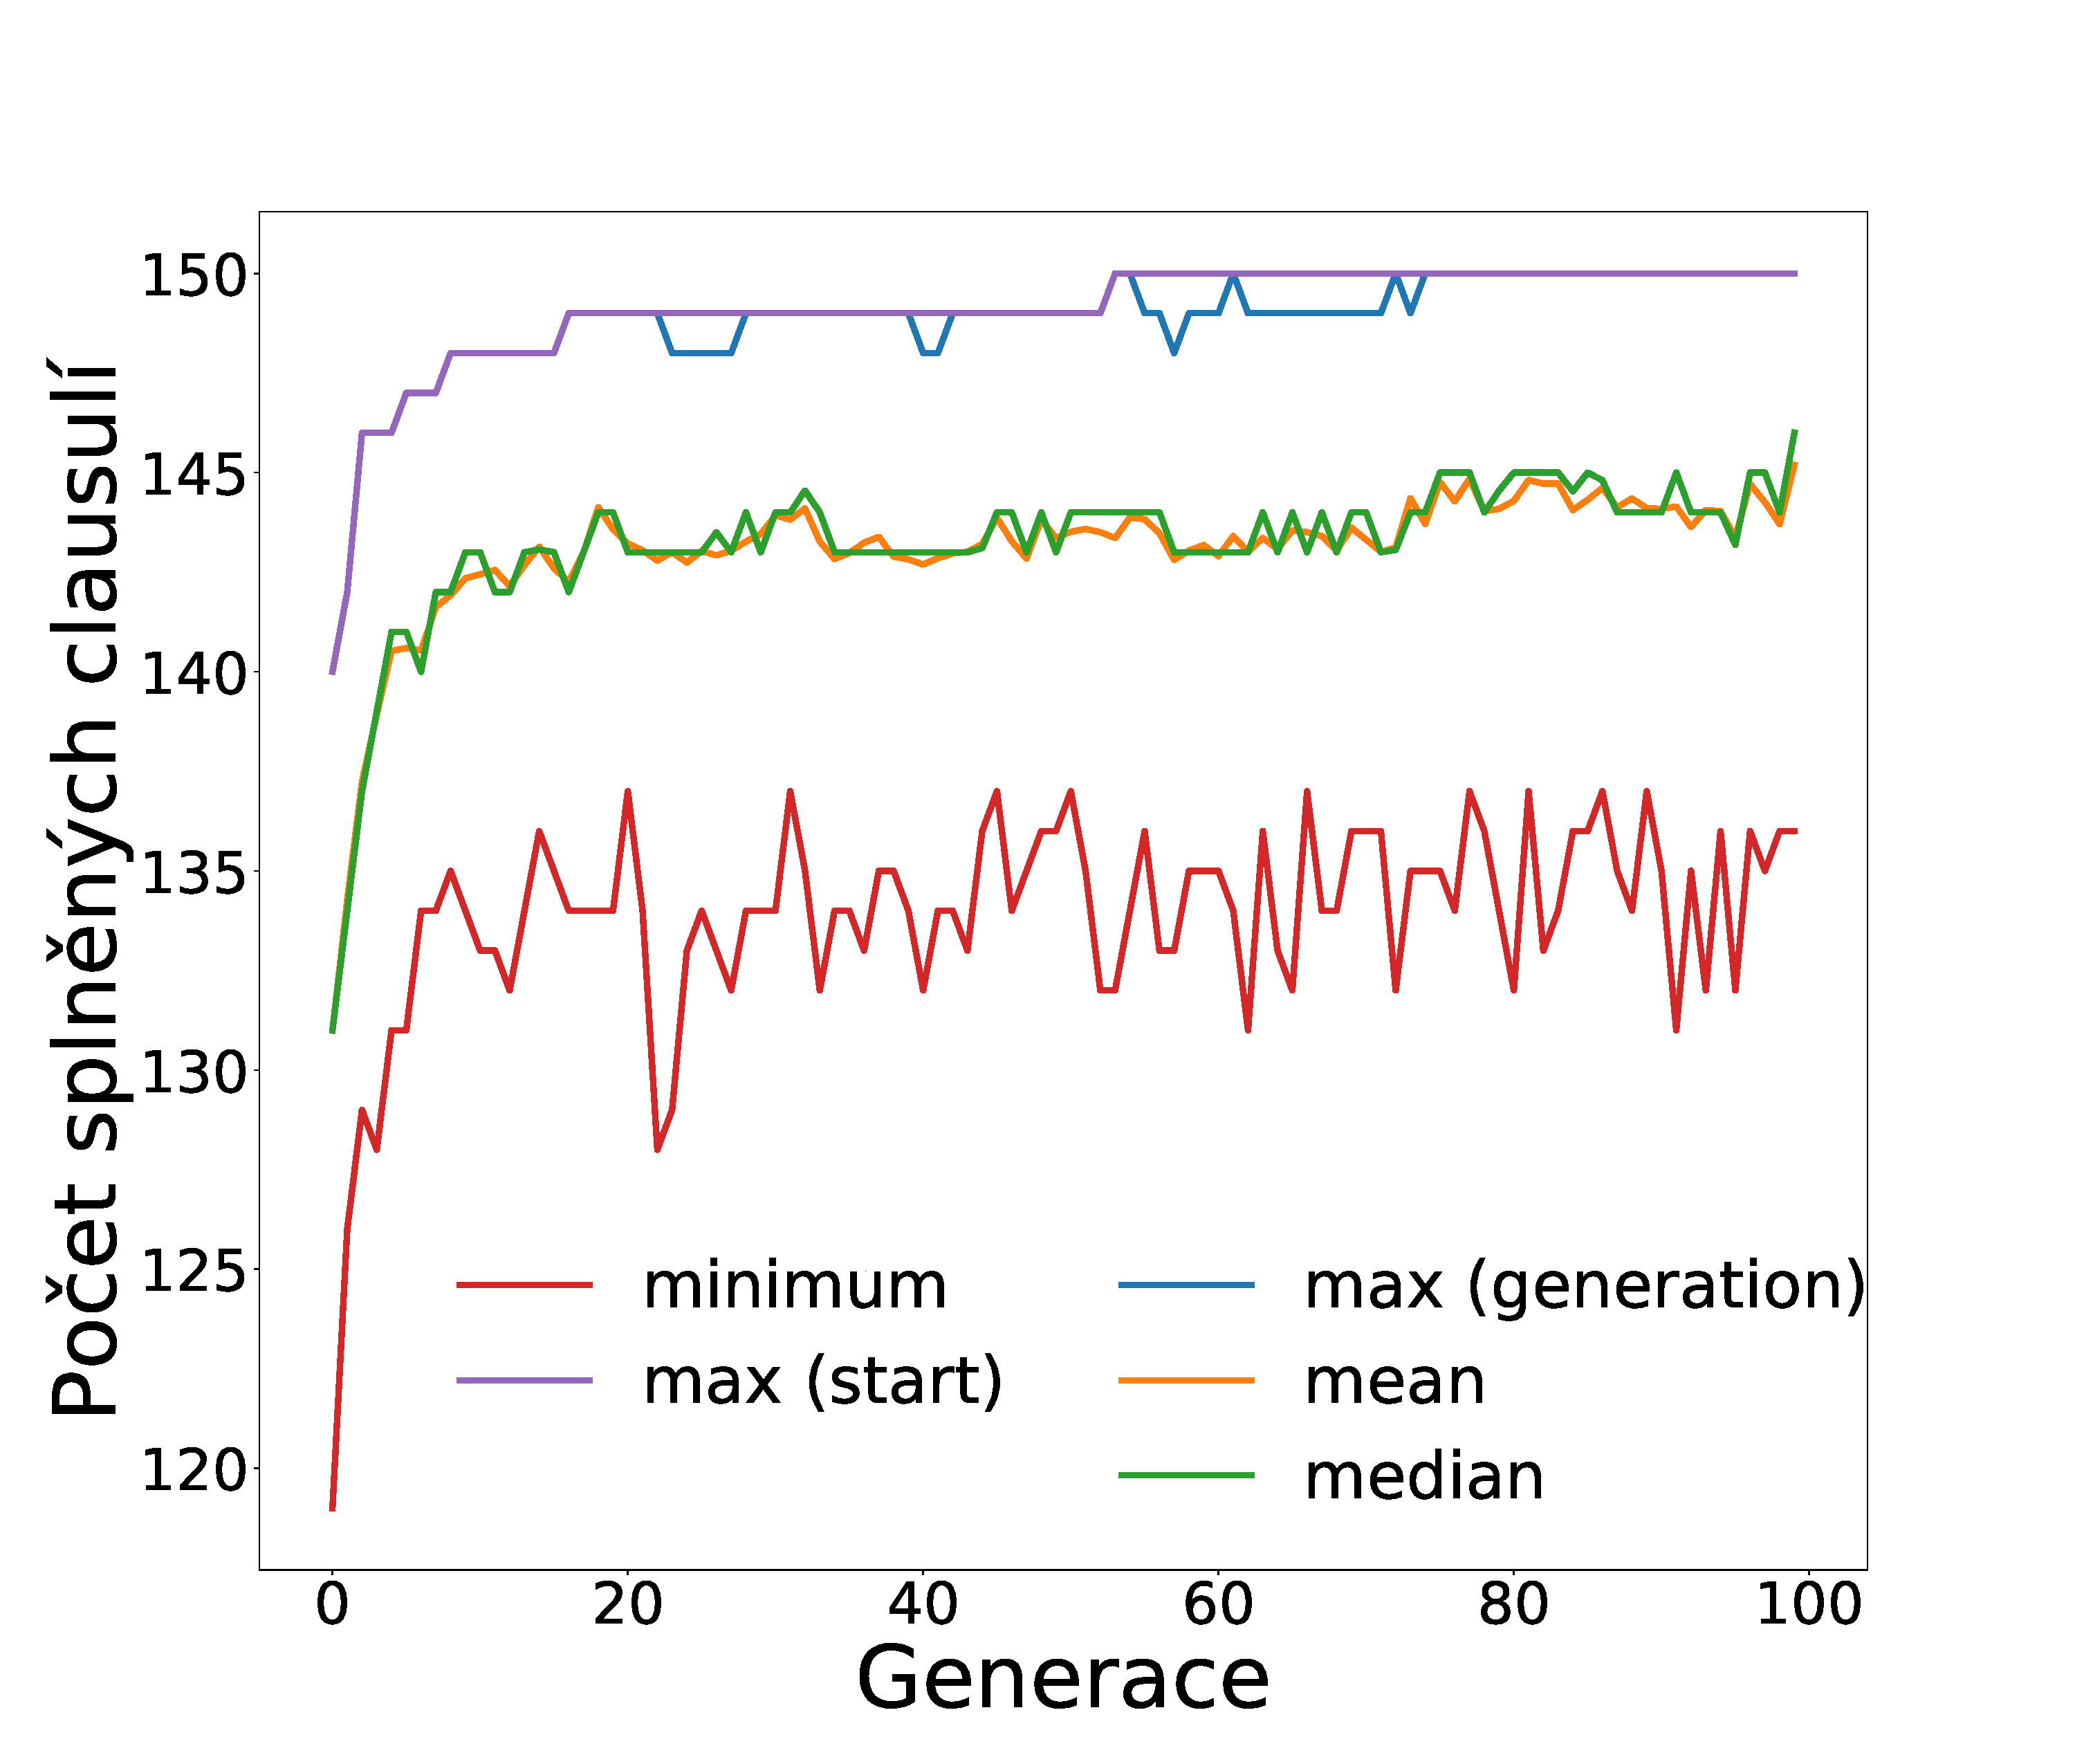
\includegraphics[width=\textwidth]{img/1c.pdf} 
    \end{minipage}
    \begin{minipage}[c]{0.32\textwidth}
        \centering 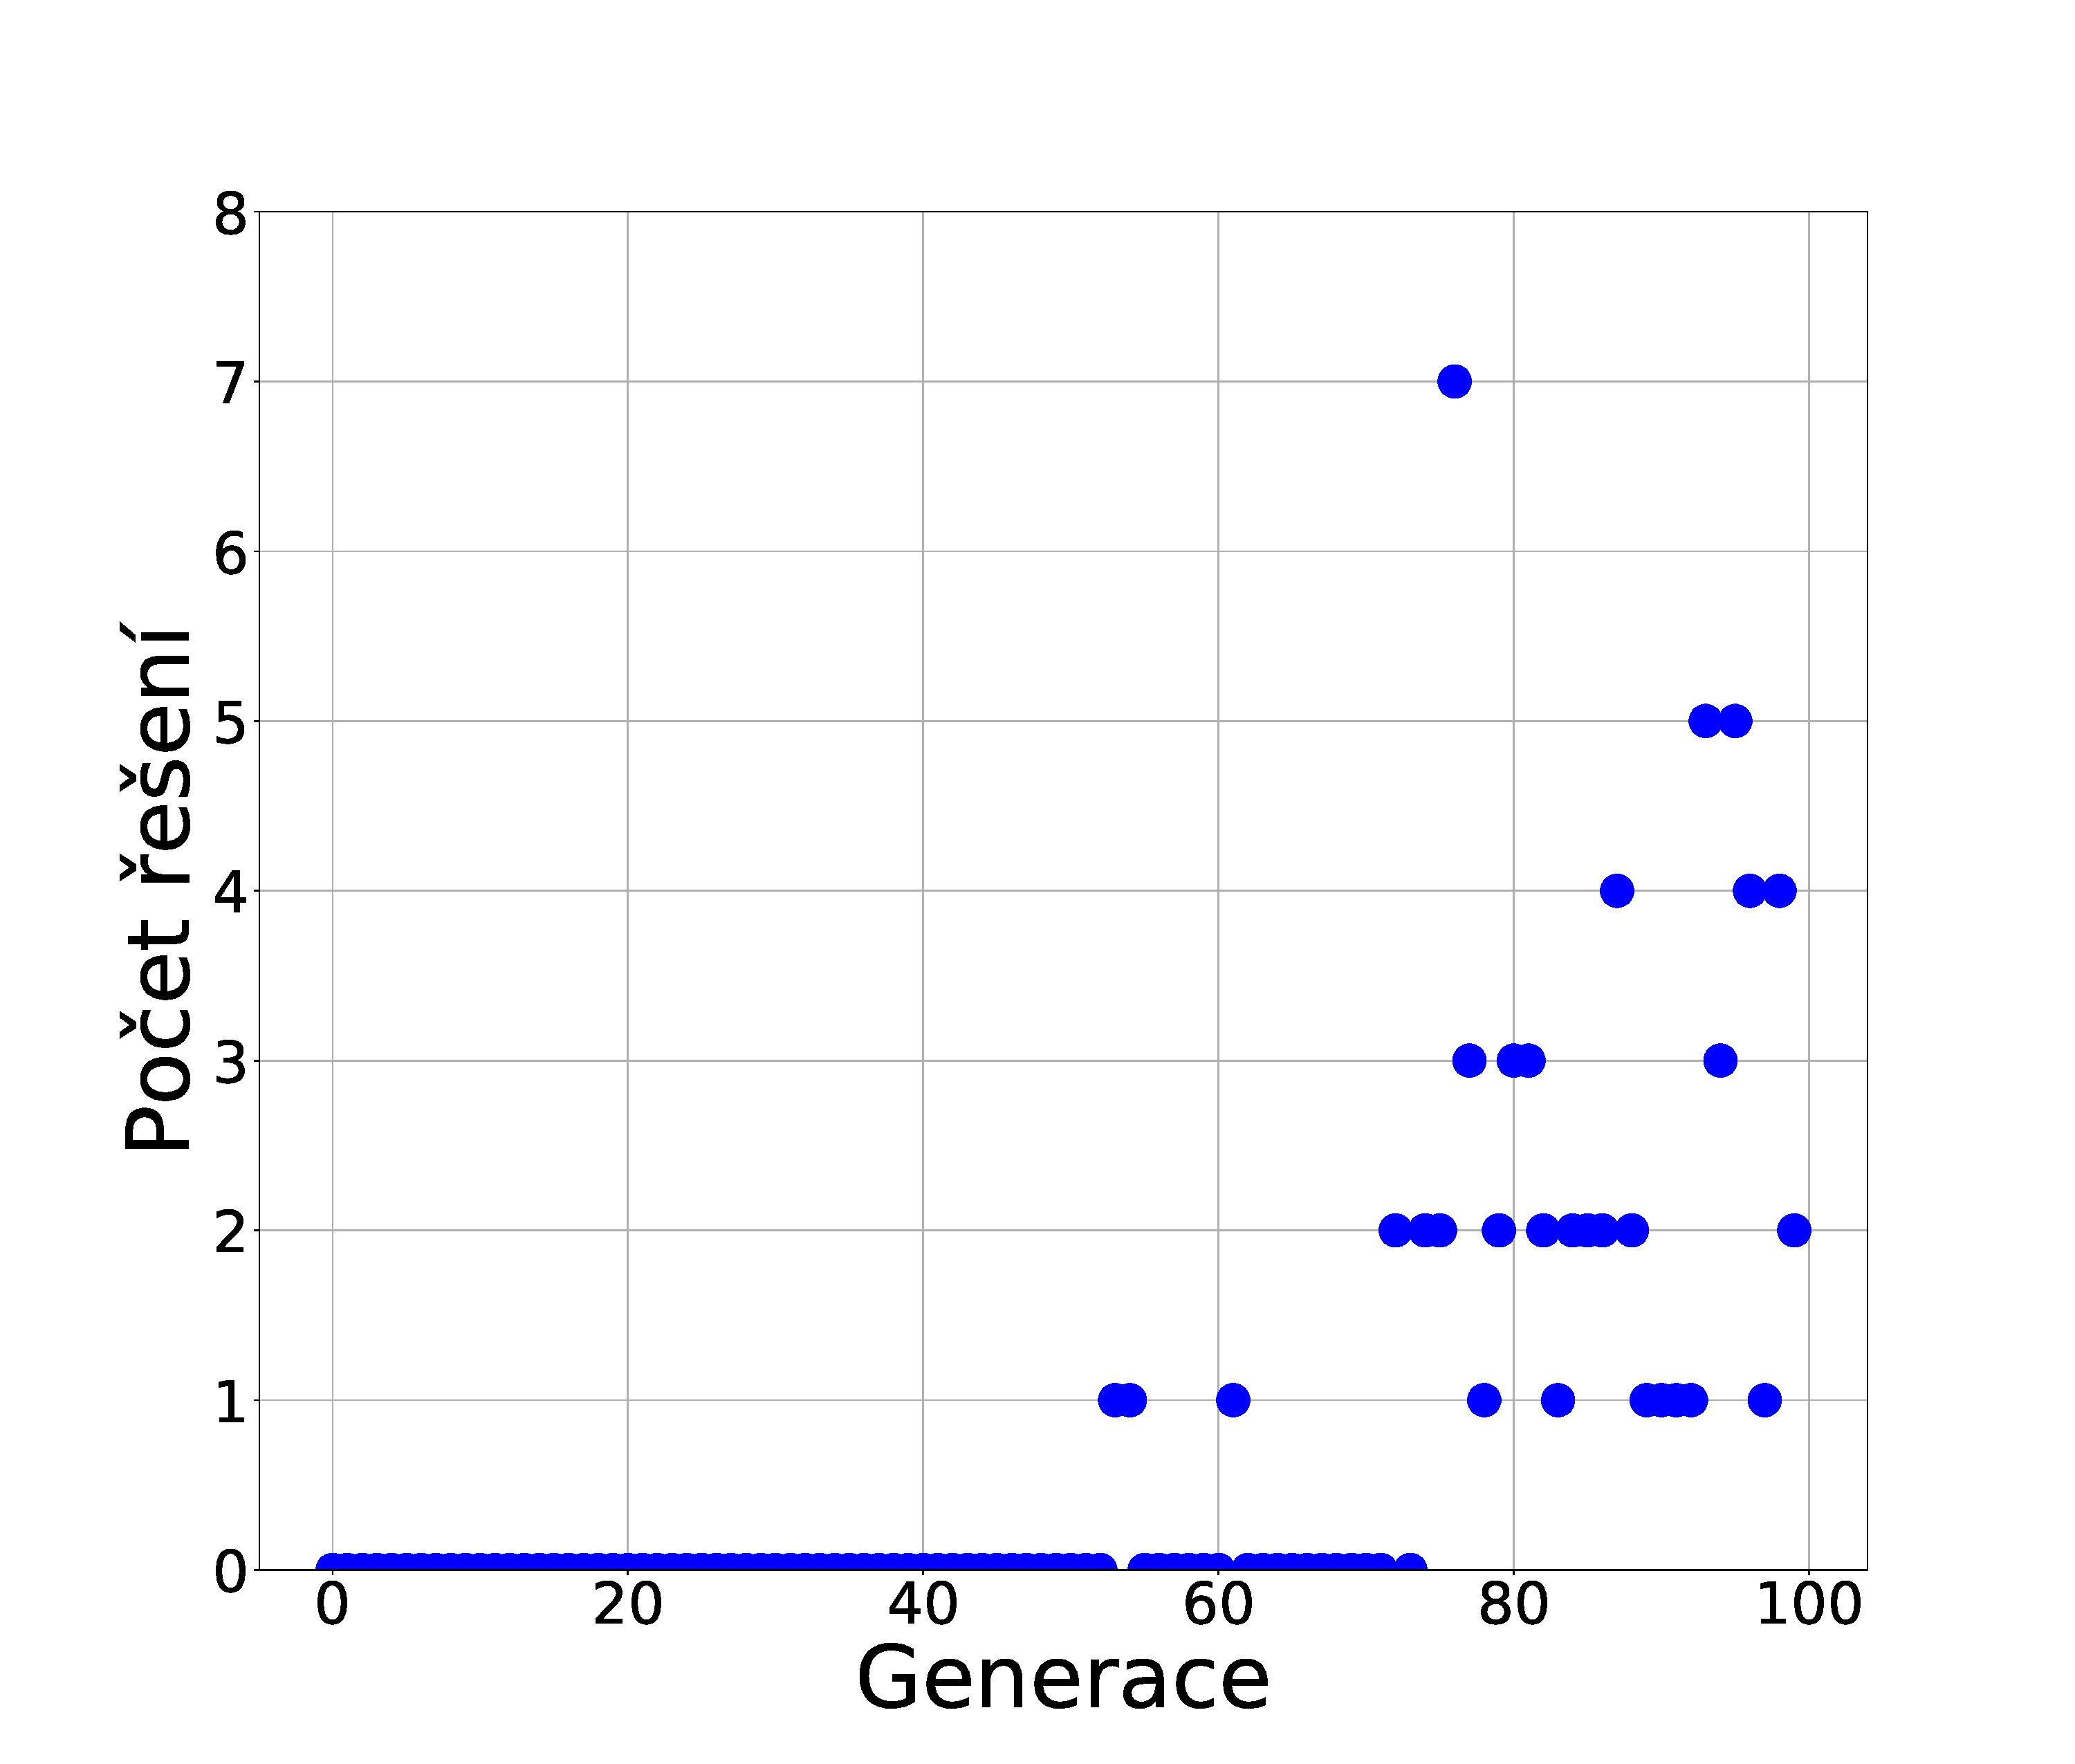
\includegraphics[width=\textwidth]{img/1s.pdf} 
    \end{minipage}
    \begin{minipage}[c]{0.32\textwidth}
        \centering 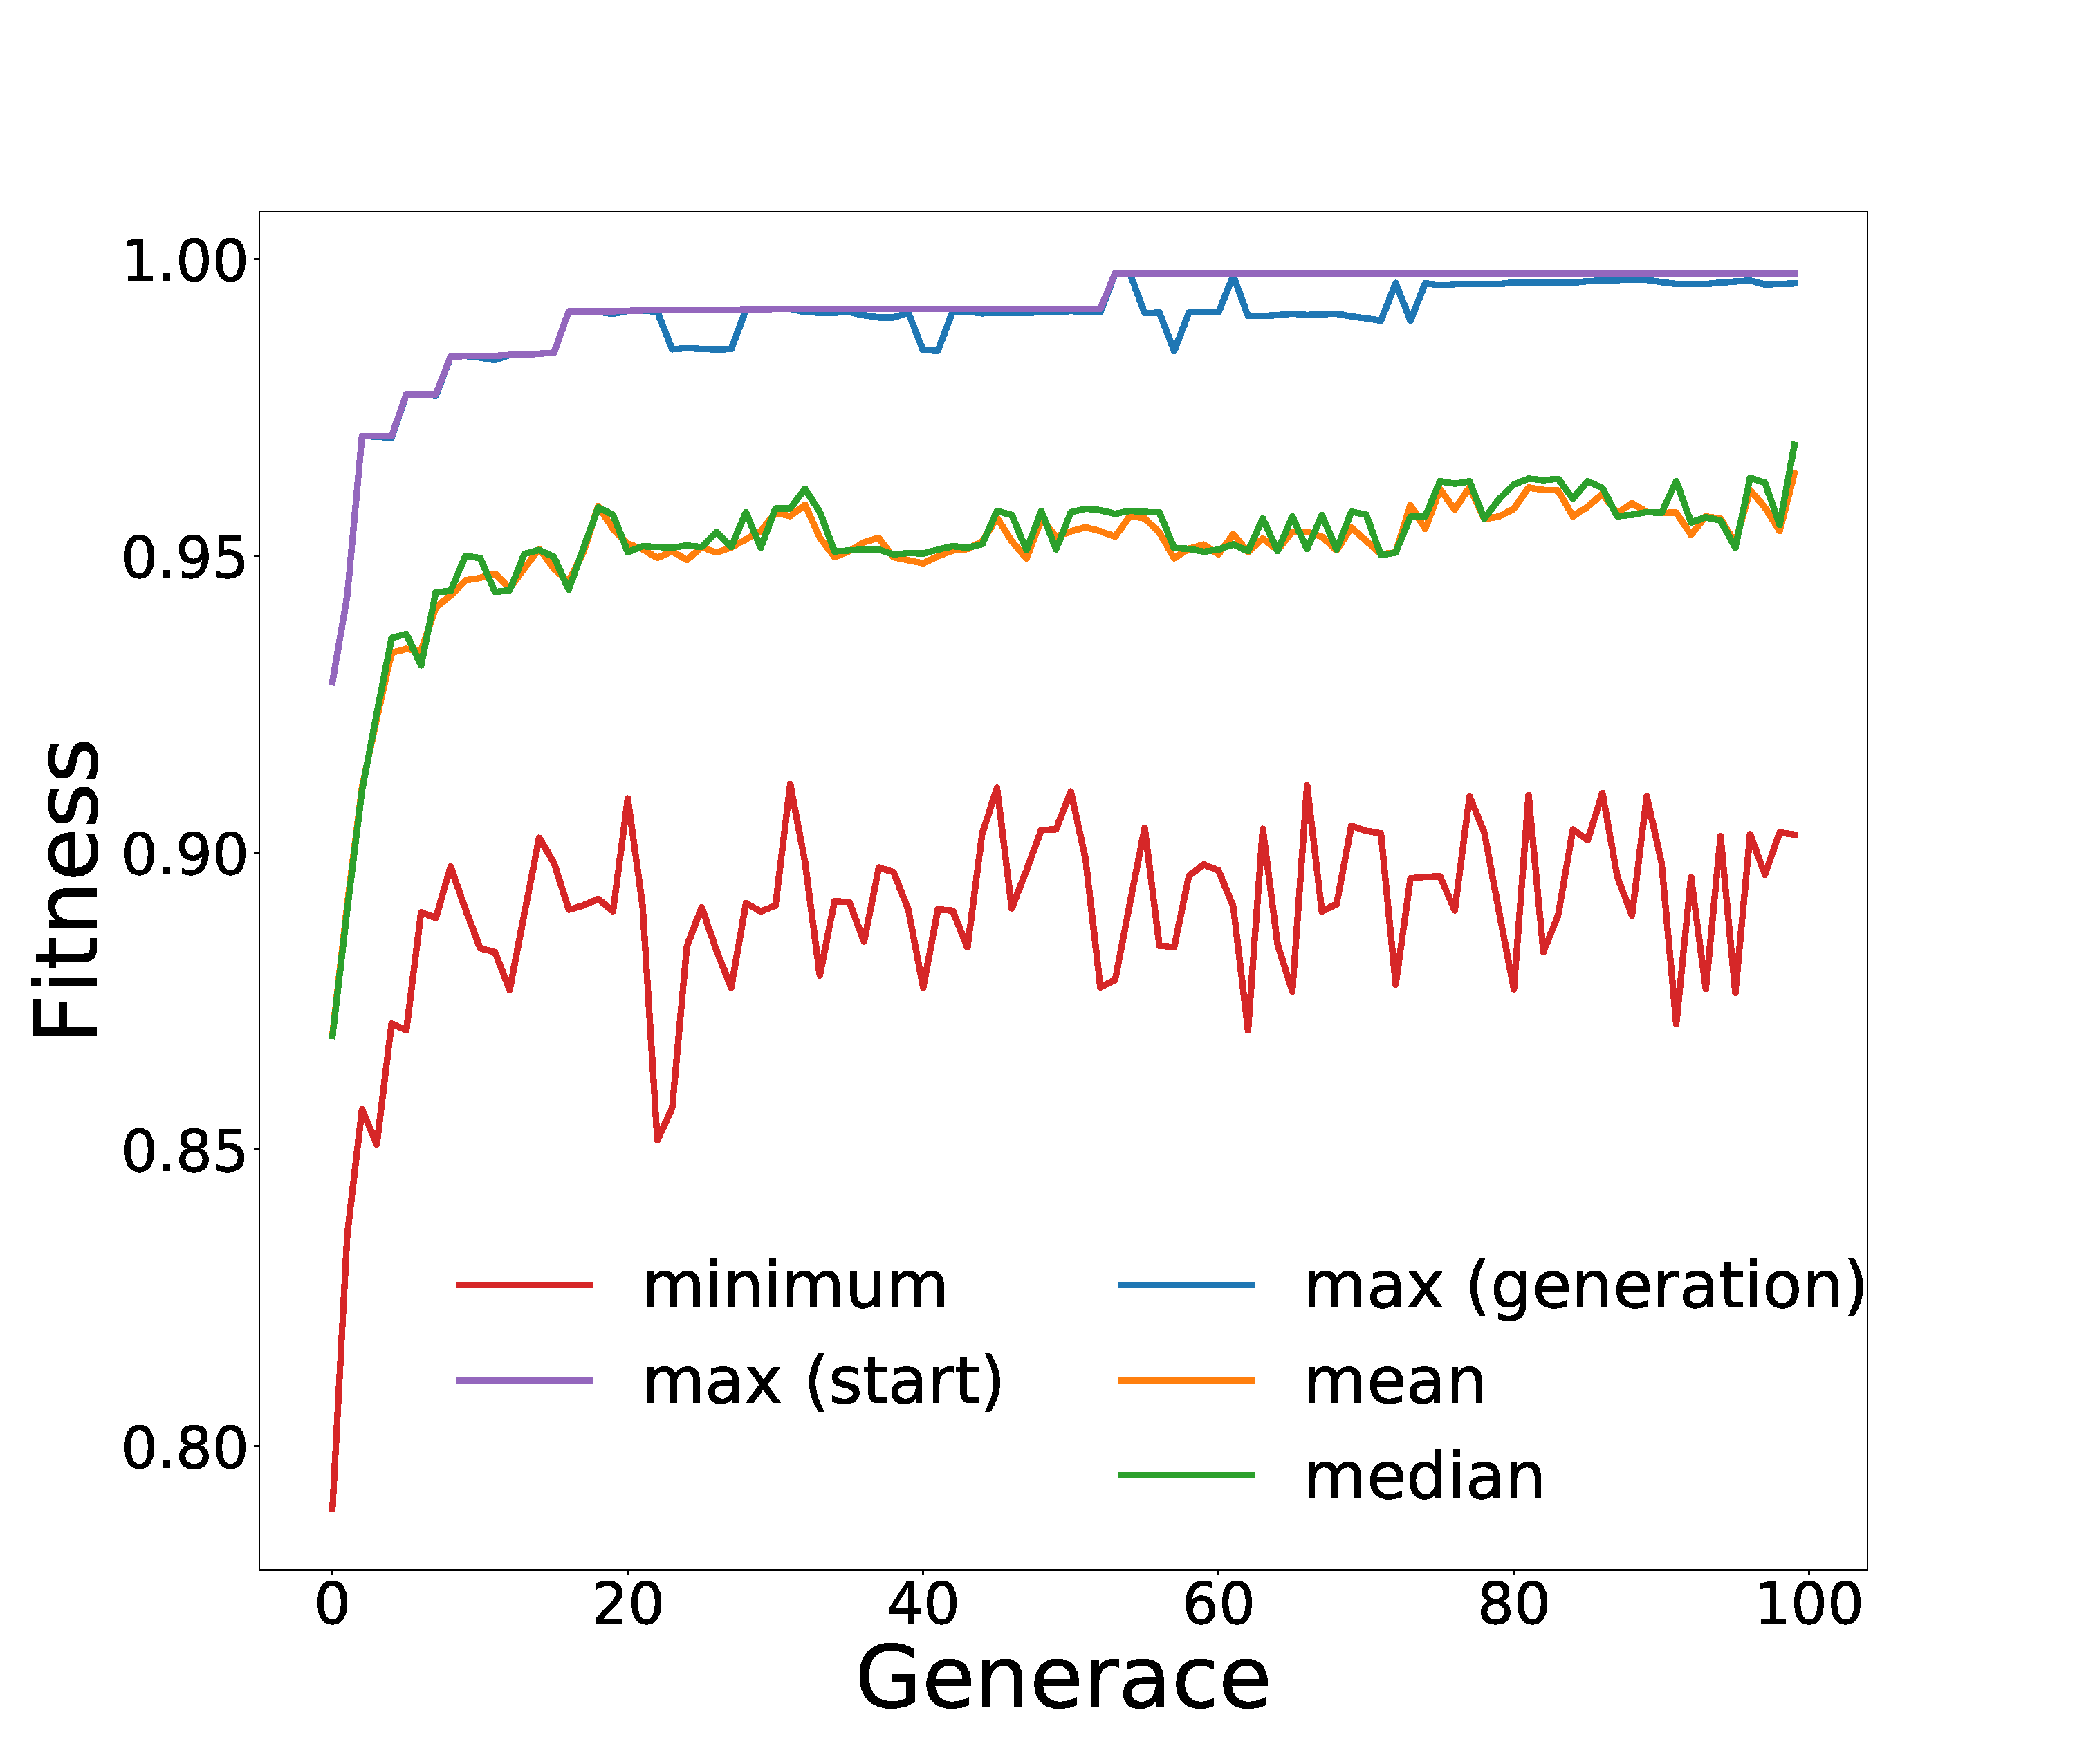
\includegraphics[width=\textwidth]{img/1g.pdf} 
    \end{minipage}
    \\
    \begin{minipage}[c]{0.32\textwidth}
        \centering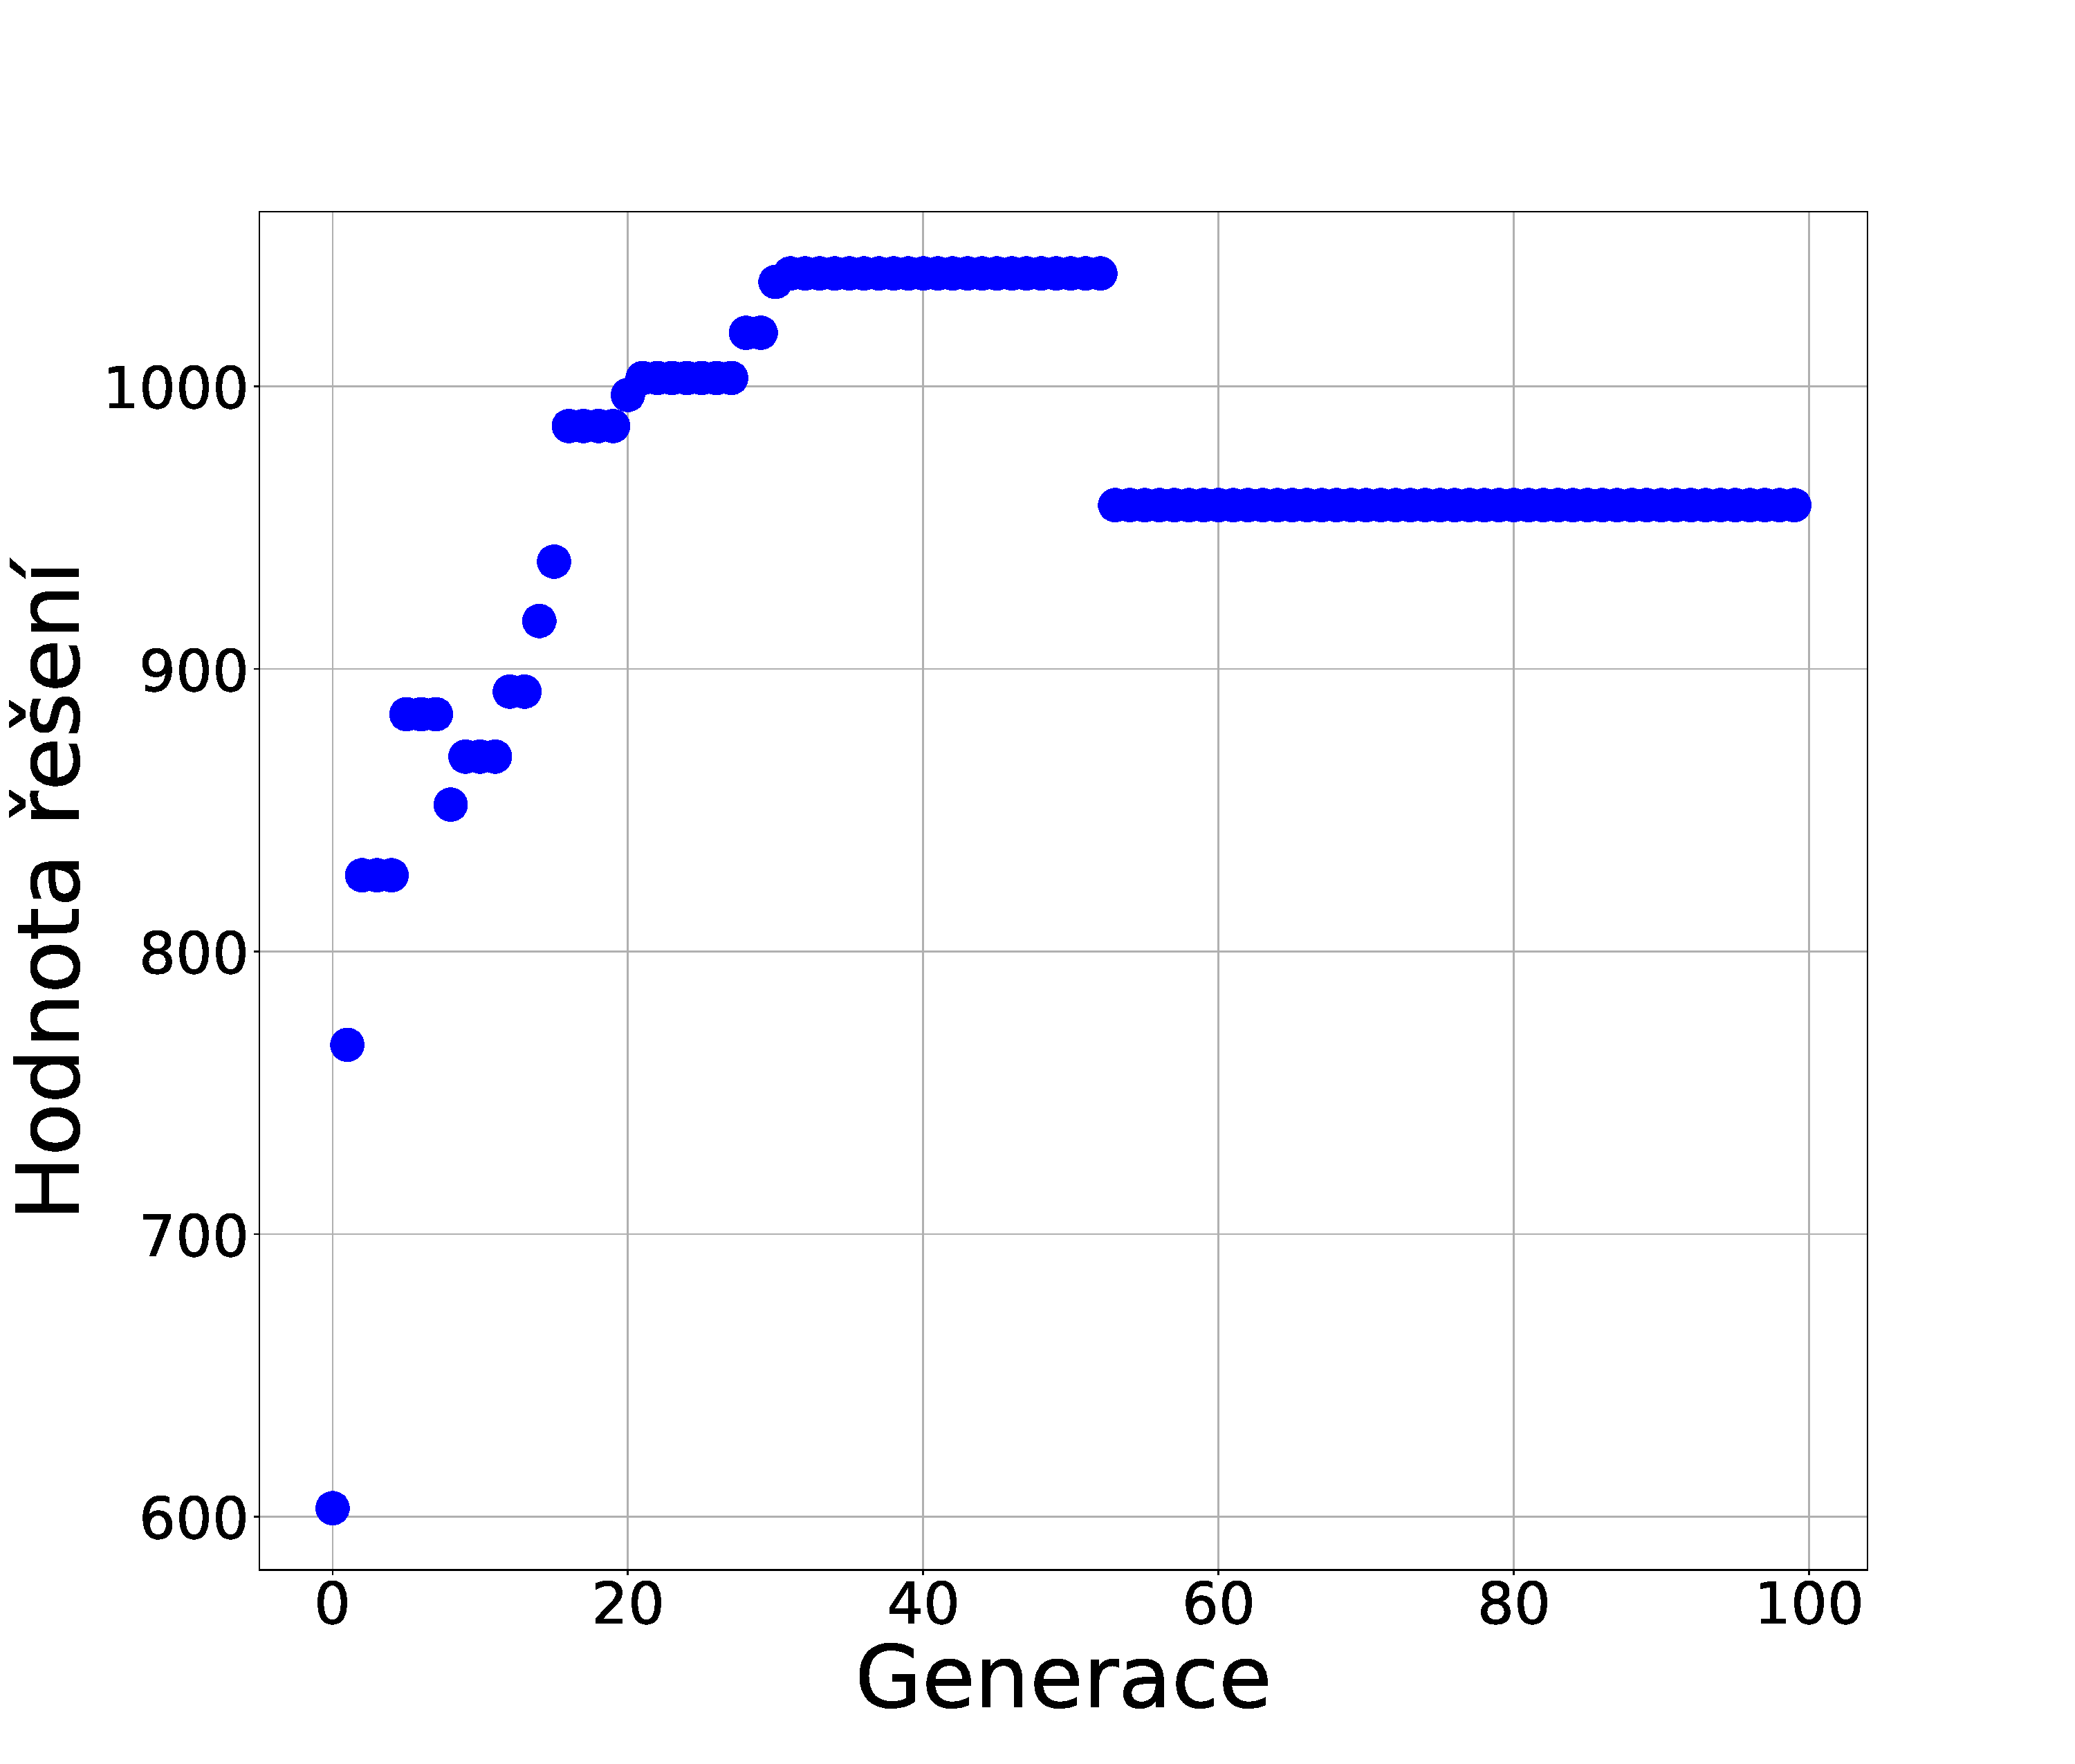
\includegraphics[width=\textwidth]{img/1w.pdf} 
    \end{minipage}
    \begin{minipage}[c]{0.32\textwidth}
        \centering 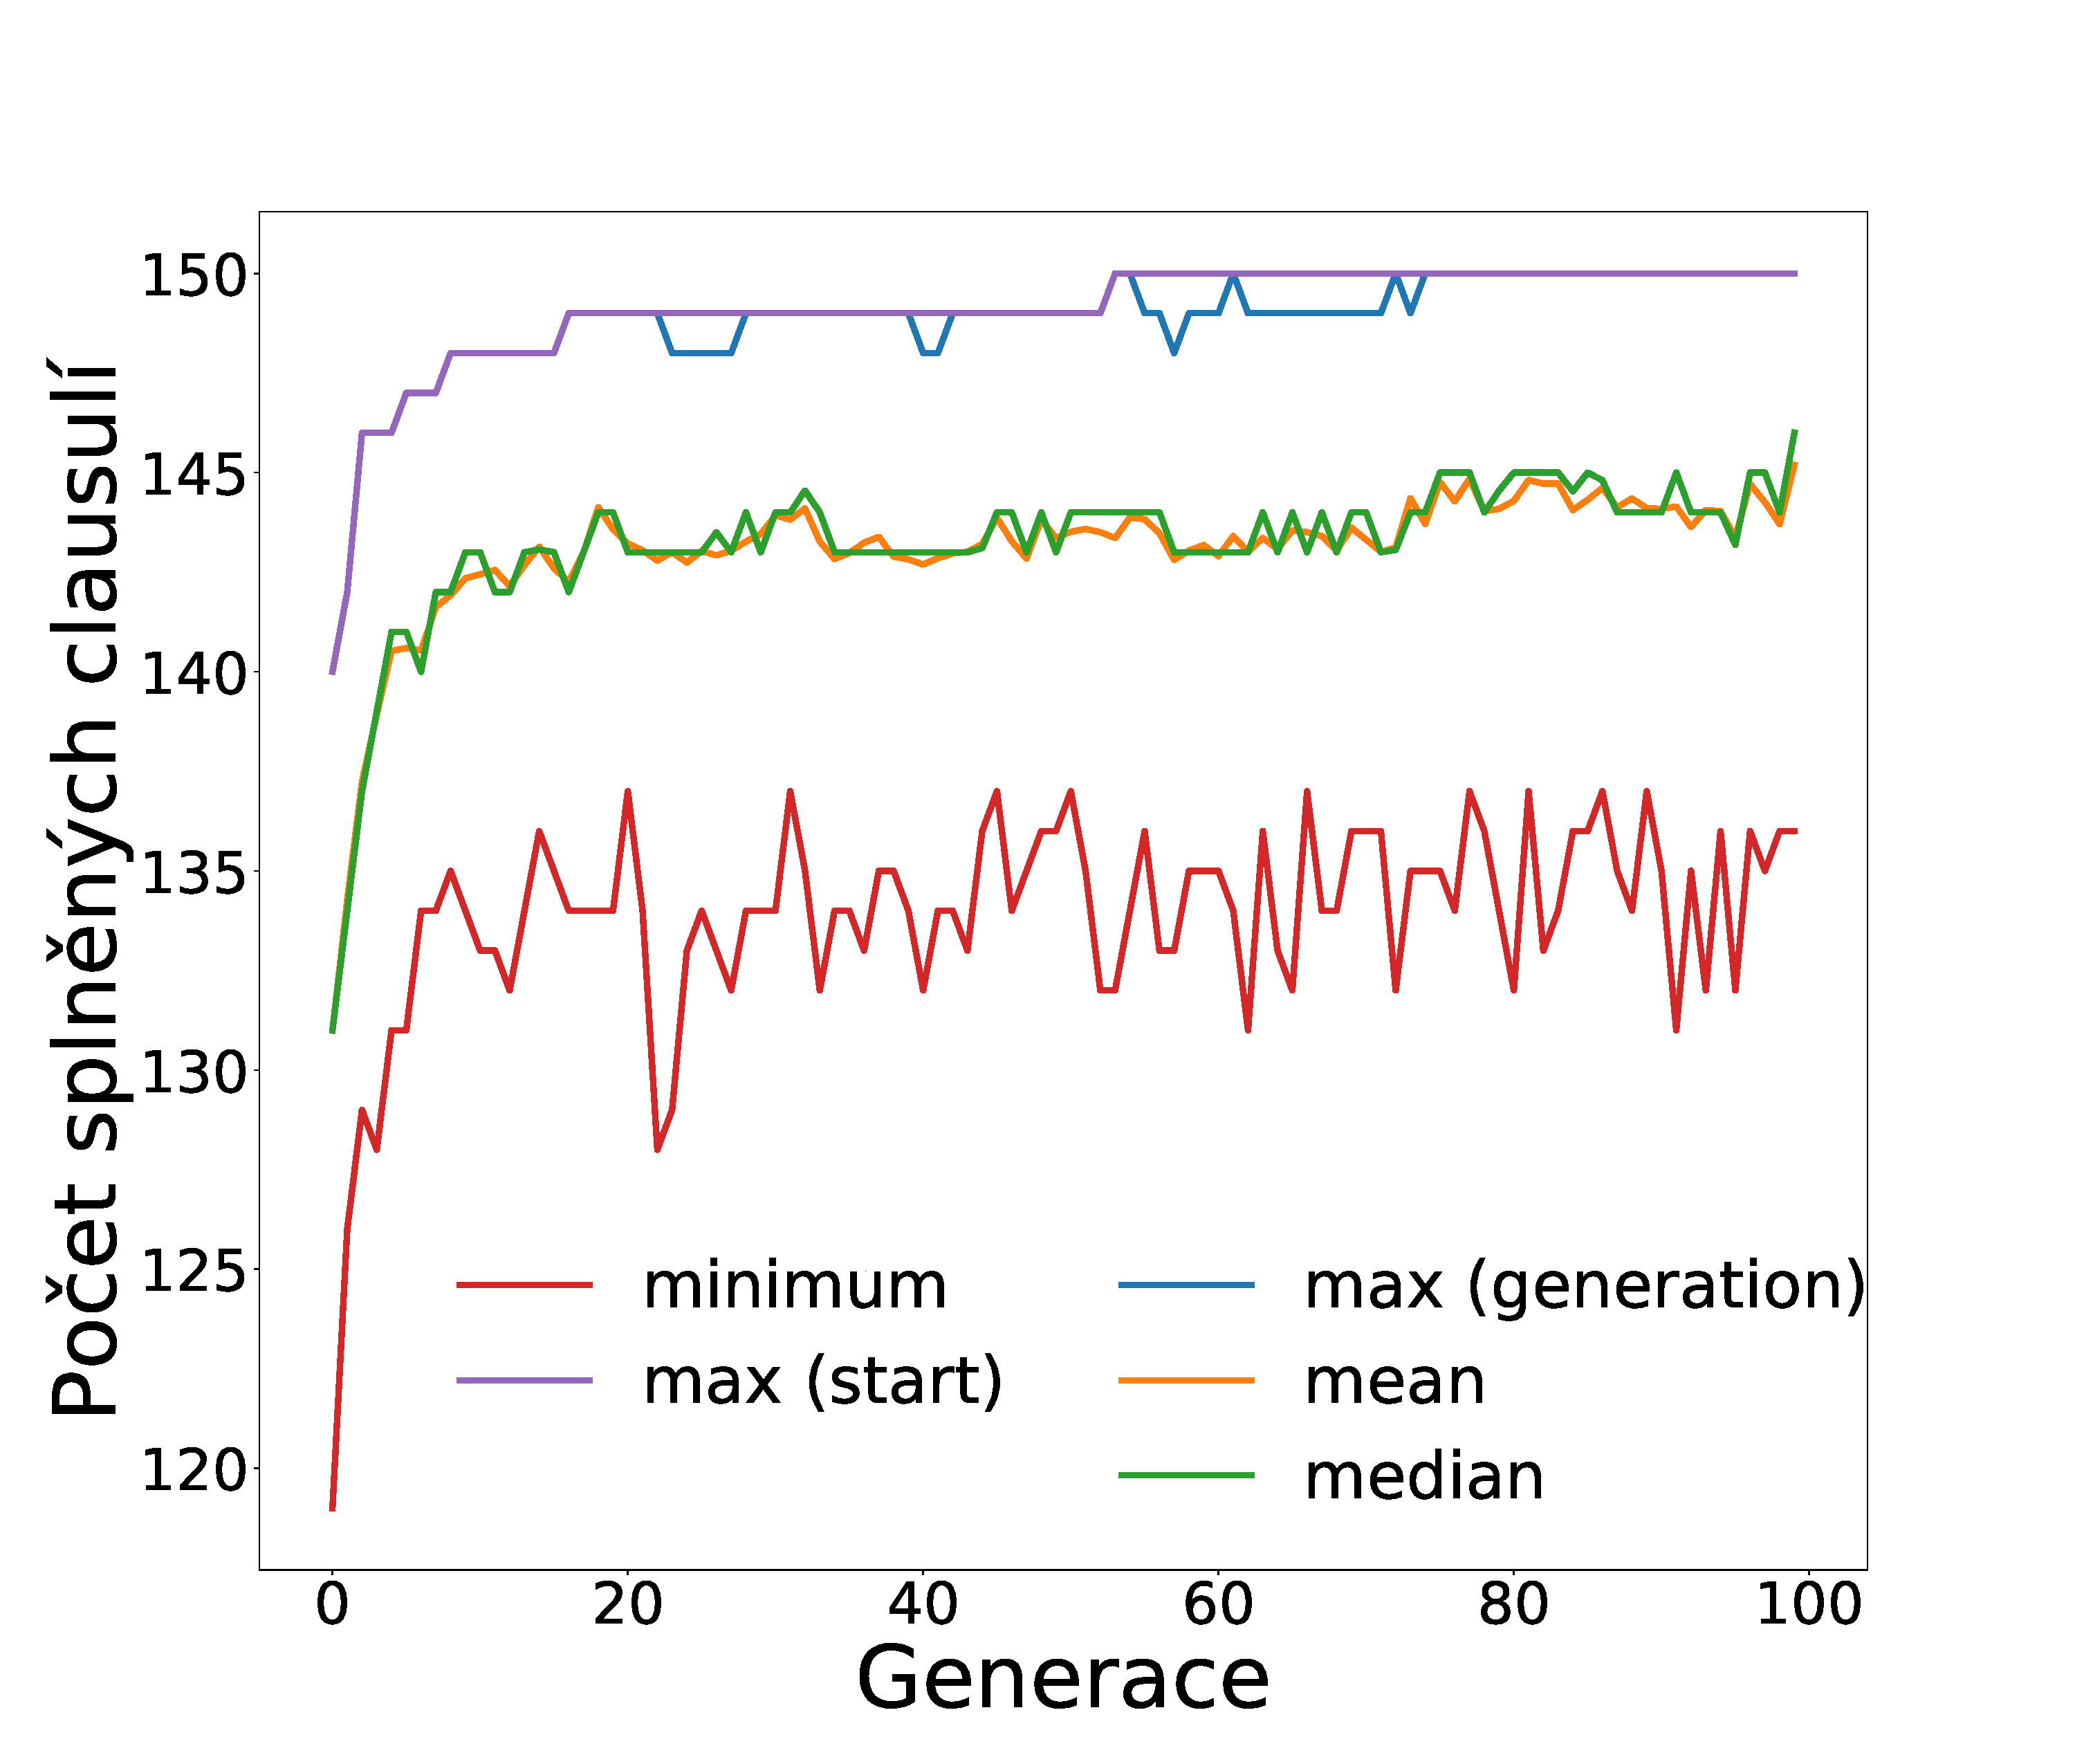
\includegraphics[width=\textwidth]{img/1c.pdf} 
    \end{minipage}
    \begin{minipage}[c]{0.32\textwidth}
        \centering 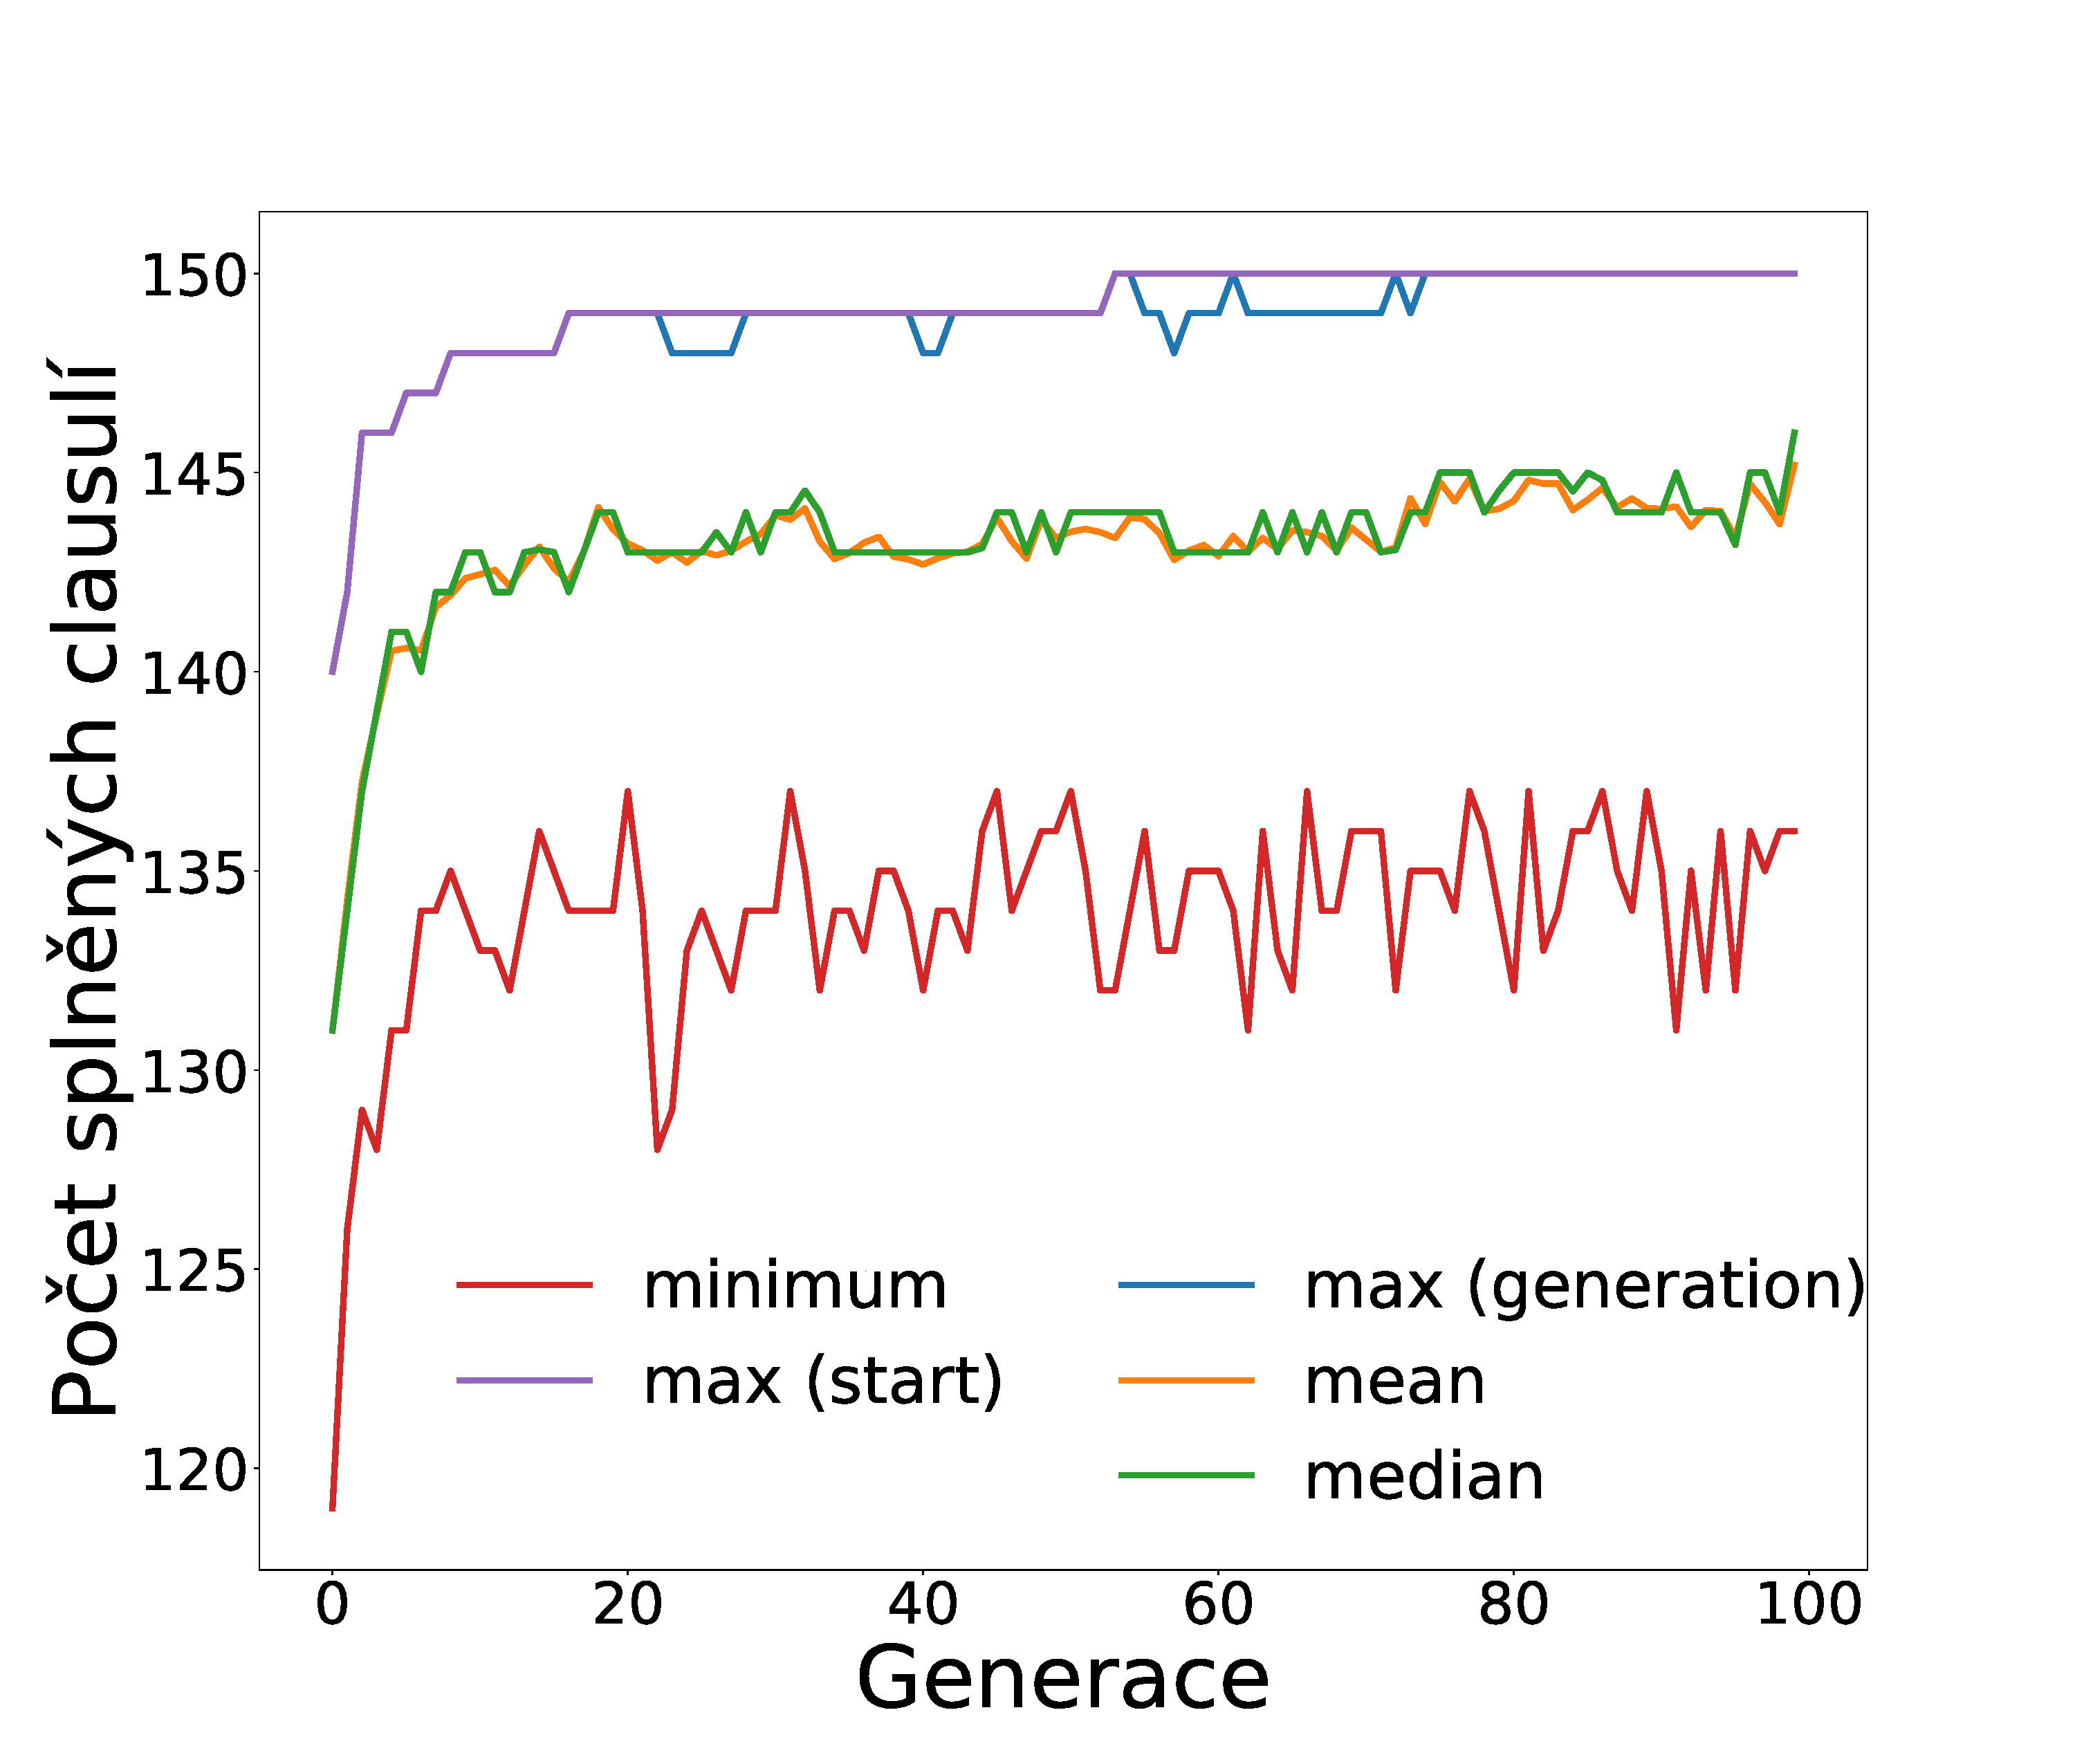
\includegraphics[width=\textwidth]{img/1c.pdf} 
    \end{minipage}
   \caption{Zde jsou uvedené grafy vývoje řešení pro vybrané hodnoty počtu iterácí na jedné teplotě. Konkrétně zleva pro hodnoty 30, 60, 120, 180, 240, 300}\label{fig:GVPC}
\end{figure} 


\section{Závěr}\label{kap:zaver}
Během experimentu jsem prozkoumal pokročilou iterativní heuristiku - simulované ochlazování. Ověřil a prozkoumal jsem závislosti této heuristiky na řídících parametrech. Parametry jsou určitě závislé na daných problémech či paramentech instancí, což je patrné i ze vzorců, kde přímo vystupuje rozdíl cen řešení. Tyto rozdíly se mohou pohybovat v různých intervalech a tomu je potřeba parametry také upravit, tedy hýbat s počáteční teplotou, která ve vzorci vystupuje jako druhý parametr. 

Simulované ochlazování je randomizovaná heuristika sloužící k prochazení prostoru, a proto může při špatném nastavení mít tendenci uváznutí v lokálních extrémech. Heuristika kombinuje přístup diverzifikace na záčatku, a následující intenzifikace je snaha o nalezení optimálního řešení. 

Ze závislostí zjištěných během experimentu je vidět, že počáteční teplota je důležitý parametr v závislosti na hodnotách ceny řešení. Pokud se ceny řešení pohybují ve velkých hodnotách bude mou snahou nastavit vyšší teploty, než pokud se budou pohybovat na nějakém intervalu a budou například normalizované. 

Parametr ochlazování je důležitý k dostatečému na vzorkování rozsahu teploty a tedy i dostatečném počtu kroků v jednotlivých fázích a to především ve fázi intenzifikace. 

Jednotlivé počty kroků na dané teplotě nám naopak dovolí prozkoumat dané okolí, ale tento parametr nemá lineární závislost na chybě, ale je dán nepřímou uměrou a volíme tak mezi relativní chybou a časovou náročností. 

Časová náročnost algortitmu je daná nastavenými parametry a s konkrétními parametry provede algoritmus vždy stejný počet kroků, tedy pro mou implementaci tohoto přístupu. Simulované ochlazování je možné například implementovat s proměným počtem kroků na jedné teplotě, který může být opět řízen nějakou jednoduchou heuristikou.

\end{document}